\documentclass[a4paper, 10pt, oneside]{book}
\usepackage[english]{babel}
\usepackage[T1]{fontenc}
\usepackage[utf8]{inputenc}
\usepackage{amsmath, marvosym}
\usepackage{booktabs}
\usepackage{titlecaps}
\usepackage{array}
\usepackage{ltxtable, longtable}
\usepackage{rotating}
\usepackage{nomencl}
\usepackage{graphicx}
\usepackage{pifont}
\usepackage{hyperref}
\usepackage{fancyref}
\usepackage{tabularx}
\usepackage{tabulary}
\usepackage[margin=1cm]{caption}
\usepackage{listings}
\usepackage[section]{placeins}
\usepackage{fancyhdr}
\usepackage[yyyymmdd]{datetime}
\usepackage{comment}
\usepackage{morefloats}

\usepackage[usenames,dvipsnames,svgnames,table]{xcolor}
\usepackage[notindex,nottoc,notlof,notlot]{tocbibind}
\usepackage{mdframed}

\usepackage{color}
\definecolor{light-gray}{gray}{0.95}
%Warnings
\newmdtheoremenv[%
	outerlinewidth = 2 ,
	roundcorner = 10pt ,
	leftmargin = 40 ,
	rightmargin = 40 ,
	backgroundcolor = light-gray ,
	outerlinecolor = black ,
	]{example}{Example}
	
\usepackage{tikz}
\usetikzlibrary{shapes, arrows, backgrounds, fit, positioning, scopes, matrix}
\makenomenclature




\lstdefinestyle{customc}{
  belowcaptionskip=1\baselineskip,
  breaklines=true,
  frame=L,
  xleftmargin=\parindent,
  language=C,
  showstringspaces=false,
  basicstyle=\footnotesize\ttfamily,
  keywordstyle=\bfseries\color{green!40!black},
  commentstyle=\itshape\color{purple!40!black},
  identifierstyle=\color{blue},
  stringstyle=\color{orange},
}

\lstdefinestyle{customsh}{
  belowcaptionskip=1\baselineskip,
  breaklines=true,
  frame=L,
  xleftmargin=\parindent,
  language=C,
  showstringspaces=false,
  basicstyle=\footnotesize\ttfamily,
  keywordstyle=\bfseries\color{green!40!black},
  commentstyle=\itshape\color{purple!40!black},
  identifierstyle=\color{blue},
  stringstyle=\color{orange},
}
\title{Genomizer}
\def\version{2.3}

\def\json{\texttt{JSON}}


\newcommand{\appName}{\textit{Genomizer}}
\newcommand{\addImage}[1]{\centering\includegraphics[width=\textwidth, keepaspectratio=true]{#1}}
\newcommand{\addScaledImage}[2]{\centering\includegraphics[scale=#1]{#2}}
\newcommand{\addImageVertical}[1]{\centering\includegraphics[height=\textwidth, angle=90, keepaspectratio=true]{#1}}
\newcommand{\addScaledImageVertical}[2]{\centering\includegraphics[scale=#1, angle=90]{#2}}
\newcommand{\refer}[1]{\autoref{#1}}
\newcommand{\addCode}[3][c]{\lstinputlisting[caption=#3, escapechar=, style=custom#1]{#2}}
\newcommand{\filePath}[1]{\texttt{#1}}
%\newcommand{\click}[1]{\ding{43} \textbf{\textit{{#1}}}}
\newcommand{\click}[1]{\textbf{\textit{{#1}}}}
\newcommand{\term}[1]{\textit{#1}}
\newcommand{\strongTerm}[1]{\textbf{\term{#1}}}
\newcommand{\serverPort}{\texttt{7000}}
\newcommand{\userstory}[2]{
\begin{tabularx}{0.95\textwidth}{|X|}
\hline
\vspace{1pt}
\large\textbf{#1} \\ 
\hline
\vspace{1pt}
#2 \\
\hline
\end{tabularx}
}

\newcommand{\addTwoImages}[4]{
\centering
\begin{tabular}{l l}
    \begin{minipage}{0.4\textwidth}
        
        \includegraphics[width=\textwidth, keepaspectratio=true]{#1} 
	\caption*{#2}

    \end{minipage}
& 
    \begin{minipage}{0.4\textwidth}
        
        \includegraphics[width=\textwidth, keepaspectratio=true]{#3} 
	\caption*{#4}

    \end{minipage}
\\ 
\end{tabular}
}

\fancypagestyle{preface}
{
	\fancyhead[L]{PREFACE}
	\fancyhead[R]{\thepage}

}


\newcommand{\addThreeImages}[6]{
\centering
\begin{tabular}{l l l}
    \begin{minipage}{0.3\textwidth}

        \includegraphics[width=\textwidth, keepaspectratio=true]{#1} 
	\caption*{#2}

    \end{minipage}
& 
    \begin{minipage}{0.3\textwidth}

        \includegraphics[width=\textwidth, keepaspectratio=true]{#3} 
	\caption*{#4}

    \end{minipage}
&
    
    \begin{minipage}{0.3\textwidth}

        \includegraphics[width=\textwidth, keepaspectratio=true]{#5} 
	\caption*{#6}

    \end{minipage}
\\ 
\end{tabular}
}

\newcommand{\addFourImages}[8]{
\centering
\begin{tabular}{l l}
    \begin{minipage}{0.4\textwidth}
        
        \includegraphics[width=\textwidth, keepaspectratio=true]{#1} 
	\caption*{#2}

    \end{minipage}
& 
    \begin{minipage}{0.4\textwidth}
        
        \includegraphics[width=\textwidth, keepaspectratio=true]{#3} 
	\caption*{#4}

    \end{minipage}
\\ 
    \begin{minipage}{0.4\textwidth}
        
        \includegraphics[width=\textwidth, keepaspectratio=true]{#5} 
	\caption*{#6}

    \end{minipage}
&
    \begin{minipage}{0.4\textwidth}
        
        \includegraphics[width=\textwidth, keepaspectratio=true]{#7} 
	\caption*{#8}

    \end{minipage}
\\
\end{tabular}
}

\setcounter{secnumdepth}{5}

\setlength{\parindent}{0pt}
\setlength{\parskip}{10pt}

\graphicspath{ {figures/}}



%\fancyhead[RO,LE]{\thepage}
\fancyhead[L]{\leftmark}
\fancyhead[R]{\thepage}
\begin{document}

\makeatletter
\renewcommand\paragraph{%
   \@startsection{paragraph}{4}{0mm}%
      {-\baselineskip}%
      {.5\baselineskip}%
      {\normalfont\normalsize\bfseries}}
      
\renewcommand\chapter{%
   \@startsection{chapter}{1}{0mm}%
      {-2cm\pagebreak}%
      {.5\baselineskip}%
      {\normalfont\huge\bfseries}}

\renewcommand\subparagraph{%
   \@startsection{paragraph}{4}{0mm}%
      {-\baselineskip}%
      {.5\baselineskip}%
      {\normalfont\normalsize\bfseries}}
 
 \renewcommand\subsection{%
   \@startsection{subsection}{4}{0mm}%
      {-\baselineskip}%
      {.5\baselineskip}%
      {\normalfont\normalsize\bfseries}}
\makeatother


\pagestyle{fancy}


\title{Tidsrapport \\ 
	Programvaruteknik \\5DV151\\
	VT-14 }
	\begin{titlepage}
		\thispagestyle{empty}
		\begin{large}
			\begin{tabular}{@{}p{\textwidth}@{}}
				%\textbf{\hfill \today} \\
				%\textbf{2014} \\
			\end{tabular}
		\end{large}
		\vspace{35mm}
		\begin{center}
			\Huge{\textbf{Technical documentation}\\ Genomizer} \\
			\vspace{10mm}
			\LARGE{Version 2.2} \\
           \vspace{5mm}
           
            Publication date: 2015-04-22 \\
            

			\vspace{70mm}
            
			\begin{normalsize}				
		 %
         %
         %	
			\end{normalsize}
		\end{center}
	\end{titlepage}


\tableofcontents


\chapter{Introduction}
\appName\ is a system for storing and analysing \term{DNA}-sequence data. It was designed for researchers in the field of epigenetics, who are interested in where on a \term{DNA} string certain proteins binds. In order to get this information, experiments are conducted and \term{raw} data files collected. These data files are then converted, in a series of steps, to files suitable for analysis. These files are hence refered to as \term{profile} data. \appName\ allows the researchers to upload \term{raw} files to a server and automate the generation of analysis data as well as store the generated analysis data in a database for later access. 


The documentation contains three main parts. Introduction chapters that explain the goal of the project as well as a non-technical description of the project implementation. The development part of the document where the current implementation of each part of the project is explained how they look and work as well as an attempt to explain why certain design choices where done. Then finally there is a big collection of appendicies that goes deeper in their explanation of certain details of the implementation as well as maintenance guides.

\nomenclature{Raw}{Collection word for files that are the result from a \textit{DNA}-sequencing machine.}
\nomenclature{Profile}{Data converted to a human readable file for analysis.}


\chapter{Target group and needs}
The \appName\ system was designed with a specific target group in mind: Epigenitic researchers. This chapter will explain the needs of these users, the problems they faced before this system was provided and the requirements that were collected and taken into account during the project.
\nomenclature{Genomizer}{Collective name for the project.}
\section{Target group}

The target group for the \appName\ system is  \term{Epigenetic Cooperation Norrland (EpiCoN)}, a diverse group of researchers at \term{Umeå University} made up of many different nationalities. Their main communication language is English.

\term{EpiCon} are involved in the research of how proteins bind to \term{DNA} strings and its effects. Experiments are carried out which yield large amounts of raw data. This information, combined with knowledge about the location of genes within a given genome, enable the researchers to gain valuable information about which proteins are active in enabling and disabling genes. These results are important in the study of how cells ''remember'' which genes should be enabled after cell division.

Previous to the \appName\ project the raw data files retrieved from experiments were manually processed by the researchers using inefficient \term{Perl} scripts. This process also involved using \term{Bowtie}\cite{BOWTIE}, a program used to unscramble the \term{DNA} data, and \term{LiftOver}\cite{LIFTOVER} which is used to adjust results to conform to different \term{genome releases}.

The researchers at \term{EpiCoN} have varying computer skills. While they all have basic computer knowledge, not all are familiar with more advanced computing tasks such as running scripts at command line level. As such, some researchers have become dependent on others to process the raw data. At \term{EpiCon} the researcher that has the knowledge to use all the scripts and software performs many of these time consuming tasks for other researchers.

From time to time students of molecular biology are interested in working with the data, however their access is limited to viewing and analysing the data. 

\nomenclature{Bowtie}{Program the preforms parsing of the raw data and counts base pairs}
\nomenclature{LiftOver}{Converts genome release versions.}
\nomenclature{Genome releases}{Constant research gives more understanding, new genome versions are often found.}

\section{Client needs}
The researchers at \term{EpiCoN} need a system to structure the large amount of genetic data they use daily. The requirements, as described below, were collected and handled as a number of \term{user stories}, each of which describe a desired function from the end users perspective. A complete list of the \term{user stories} are presented in \fullref{chap:userstories}. %When discussed below the title of the relevant \term{user story} will be used.
A overview of the requested system may be seen below in figure \ref{fig:requestOverview}. Where orange colored nodes are must have features while gray nodes are visions of the clients that may be implemented if time allows for it.

There are three main data types used in the research and that the system should handle: \term{raw}, \term{profile} and \term{region} data. \term{Raw} data is the raw output from an experiment and cannot be analysed directly. It is first processed to so called \term{profile} data. \term{Profile} data describes the amount of reads found for every base--pair in an organism's genome. \term{Region} data is further processed \term{profile} data consisting of the regions where every base--pair's read strength is above a given threshold and fault tolerance. The region gets a value based on the average of the base-pair reads for the given region.

\nomenclature{Region}{Region data is small parts of the profile data.}
\begin{figure}[h!]
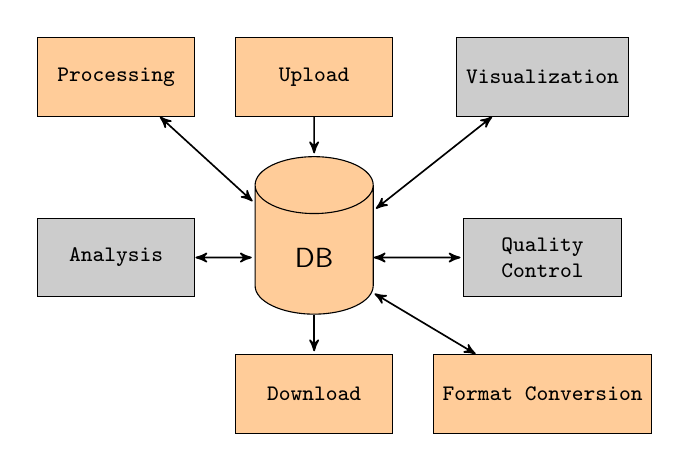
\begin{tikzpicture}[ 
	font=\sffamily,
  every matrix/.style={ampersand replacement=\&,column sep=0.5cm,row sep=0.5cm},
  db/.style={cylinder, shape border rotate=90, draw, fill=orange!40, minimum height=2cm, minimum width=1.5cm},
  must/.style={rectangle, draw, fill=orange!40, minimum height=1cm, minimum width=2cm, font=\ttfamily\footnotesize},
  vision/.style={rectangle, draw, fill=gray!40, minimum height=1cm, minimum width=2cm, font=\ttfamily\footnotesize}, 
  both/.style={<->,>=stealth',shorten >=1pt,semithick,font=\sffamily\footnotesize},
  to/.style={->,>=stealth',shorten >=1pt,semithick,font=\sffamily\footnotesize},
  every node/.style={align=center}]
  
\matrix{
	\node[must] (proc) {Processing}; \&
	\node[must] (add) {Upload}; \&
	\node[vision] (visual) {Visualization}; \\
	\node[vision] (analys) {Analysis}; \& 
	\node[db] (B) {DB}; \& 
	\node[vision] (quality) {Quality\\ Control}; \\
 	\& 	\node[must] (extract) {Download}; \&
 	\node[must] (format) {Format Conversion}; \\
	};
	
	\draw[both] (proc) -- (B);
	\draw[to] (add) -- (B);
	\draw[both] (visual) -- (B);
	\draw[both] (analys) -- (B);
	\draw[both] (B) -- (quality);
	\draw[to] (B) -- (extract);	
	\draw[both] (format) -- (B);

\end{tikzpicture}
\caption{Overview of targeted system}
\label{fig:requestOverview}
\end{figure}

\subsection{Upload \& Download}

When conducting experiments the researchers generate \term{raw} data that generates what they call \term{Raw}-files. These files along with profile data, region data and genome release data may be added and related to an experiment. The requested functionality is to be able to upload these files to the database from multiple sources. The sources may be directly from an experiment conducted by the researchers or from official publications.

When results are published in scientific articles the \term{raw} data from the experiments are often also provided. One location where these \term{raw} data files can be published is the \term{GEO} (\term{Gene Expression Omnibus}) database. A desire to be able to initialize a upload to \appName with the source of the upload beeing  \term{GEO}.
\nomenclature{GEO}{Centralized database where article data can be found.}

\subsection{Database}
The \texttt{Database} module requested has the purpose to archive experiment data in a way of easy access. To allow for this the experiments and files associated with them needs to have information vital for good readability. This is solved with the help of annotations. The reaserchers must add annotations to files related to an experiment.
This data is the foundation for further research and so must be stored securely. To ensure security the client requested a system for authorization that protects the data from outside tampering. To protect against hardware failure there exists a request for a backup system.

\subsection{Processing}
The unordered \term{raw} data gained from an experiment requires processing in order to be analysed. The researchers have written a number of scripts and, when combined with the \term{BowTie} algorithm, generate \term{profile} data. In this format the \term{DNA} pieces are ordered and mapped to the \term{DNA} string. It is important that the system automates this process so that all researchers can easily process the large \term{raw} files.

As new discoveries are made in the area, new standards for the order of the base pairs in a \term{DNA} string are set. This results in a new \term{Genome Release} for a specific species. These are obtained as a set of files specifying this order and are used in the processing of \term{raw} data. \appName\ must support the uploading of new sets of \term{genome release} files to be used in processing otherwise the system will very quickly become outdated. 

It would also be an advantage if the system could carry out further processing from \term{profile} to \term{region} files.

After processing, the resulting data files should be annotated and saved in the database alongside their parent files. It is important that the parent files remain traceable and that the parameters used in processing are saved so that the process can be repeated and confirmed.

\subsection{Format Conversion}
\appName\ should also provide a way to convert \term{profile} data files between different genome releases. This involves the ability to upload new \term{Chain Files} which enable conversion using \term{LiftOver} and the embedding of this program.

It is not uncommon for errors in a new release to be discovered after publication. It is therefore also important to store files generated using older genome releases for some time after a new release is published.

\nomenclature{Chain files}{Genome release files with small alterations to previous genome releases.}


%\begin{comment}


\chapter{Service description}



This chapter will present an overview of the services that the \appName\ system provides. 

\section{Usage}

\begin{figure}[h]
\addImage{genomizerDiagramServiceDescription.png}
\caption{Communication diagram of the product}
\label{con_serviceDescription}
\end{figure}
	
In order to give the users flexibility when using the service there are clients for many different platforms (Windows, Linux, OSX, Web, Android and iPhone). 
When a user chooses a given task, for example start \term{raw} to \term{profile} processing, that task is sent by internet to the server as shown in \refer{con_serviceDescription} which will handle the request and send a response back to the user.

The main purpose of the \appName\ system is to centralise all data. To enable this a user can annotate and upload data to the server using both desktop and web based clients. 
Advanced database searches can be performed on the annotations to find previously uploaded data. When the required data is found the user can choose to download the files or schedule them for processing on the server.

\section{Processing}
Users can schedule various processing procedures on different data sets. This is carried out on the server to avoid heavy workload on the clients. The processing carried out between \term{raw} data and \term{profile} data involves a number of different steps. The user can choose which steps are carried out and the various parameters used.

\section{Genome releases}
Users can upload new genome release files and use them in the processing of \term{raw} to \term{profile} data.

\section{Mobile}
The mobile applications enable the searching of files in the database and the scheduling of processing procedures for the conversion of \term{raw} to \term{profile} data.

\section{Annotations}
A user with access to the \term{Systemadmin} page can add or delete annotations used to store information about experiments.




\chapter{User manual}
%User manuals for the different clients. Directed towards users (includes everyone). Start with subsection here.

%This chapter explains to the user how each client should be used. It starts with the desktop and web clients. These clients are the main clients that can handle the main features. Then comes instructions for the mobile clients that are designed to search for files and tell the server to convert them.

This chapter explains how you use each of the \appName\ clients. First instructions on how to use the desktop and the web clients are presented. These are the clients which provide the most functionality. The mobile clients are more lightweight and offer a subset of the functionality presented by the desktop client. Instructions on using the smartphone applications for \term{Android} and \term{iOS} are presented in their on sections at the end of the chapter. 


\section{Desktop}
This is a user manual for the desktop client. It will provide guides on how to 
use the client and the different functionalities it holds. The screen shots 
shown in this document are made from a Linux machine, but the application 
also runs on Windows or Mac, and will follow the design principles thereafter. 
Because of this, some details of the look of the client may vary, but the functionality is the same.

\subsection{Login and startup}
When you start this application the first thing that's displayed is a login screen, as illustrated in \refer{fig:des_login-pic}. In this screen you enter your username, password and the IP-Address for the server and then press enter or login to enter the \appName\ Desktop.

\begin{figure}[htb]
	\addScaledImage{0.5}{des_login_picture.png}
	\caption{Screenshot of the login screen.}
	\label{fig:des_login-pic}
\end{figure}
The application is built with tabs, as illustrated below in \refer{fig:des_tabs-view}. Each tab contains separate features of the application. There are five tabs: Search, Upload, Process, Workspace and Administration.
\begin{figure}[htb]
	\addImage{des_tabs.png}
	\caption{Illustration of the different tabs of \appName Desktop and displaying the Search tab.}
	\label{fig:des_tabs-view}
\end{figure}
\FloatBarrier

\subsection{Search}
The first tab that meets the user after logging in is the Search tab, illustrated in \refer{fig:des_search-query}. The Search tab uses the same query building technique as the “Pubmed Advanced Search Builder”\cite{des_3}. It has one text field where you either can type in the query yourself or you can use the query builder below it to build the query. To switch between manually editing the query and using the query builder there are two radio buttons to the left of the text field. Each row in the query builder has at most five components. These are a logical expression, an annotation name field, a free text field or a drop down menu to insert search words, a minus button and a plus button. The plus button is only available in the last row and it adda another row to the query. The minus button is used to remove a row and it exists on every row except if there is only one row in the query. The logical expressions combines the annotations, so they are available in every row but the first.
By writing in the annotation text field or selecting a value in the drop down menu you can specify the query the row will produce. Together each row builds a full query. As illustrated in \refer{fig:des_search-query} below.
\begin{figure}[htb]
	\addImage{des_search_tab.png}
	\caption{Illustration of a query, made by the query builder.}
	\label{fig:des_search-query}
\end{figure}
\FloatBarrier
\subsubsection{Search results}
When the search button is pressed the search tab will change it's view to display the search results as illustrated in \refer{fig:des_search-results}. The results are displayed as experiments in a tree table. Each row is an experiment that cn be expanded to show more information and the files associated with the experiment. The tree table can be sorted both vertically by clicking the headings and horizontally by dragging and dropping the columns. The user can choose which columns to display by using the menu in the upper right corner of the table. In the same menu there are also buttons for expanding and collapsing all experiments in the search results. To go back to the previous view, the user can click the \emph{Back} button. There is also a button called \emph{Add to workspace} for adding the selected files or experiments to the workspace. The last button, \emph{Upoad to experiment} is used to upload more files to an experiment.

\begin{figure}[htb]
	\addImage{des_search_res.png}
	\caption{Illustration of search results.}
	\label{fig:des_search-results}
\end{figure}
\FloatBarrier

\subsection{Upload}
If the user needs to upload files to the database it can be done through the upload tab. When the tab is pressed the user gets presented with a button to create a new experiment shown in figure \ref{fig:des_upload-tab}.
\newpage
\begin{figure}[h!]
	\addImage{des_upload_tab.png}
	\caption{Illustration of the starting view of the upload tab.}
	\label{fig:des_upload-tab}
\end{figure}
\subsubsection{Existing experiment}
\label{sec:des_exists}
In order to upload files to an existing experiments the users needs search for the experiment in the search tab and then press the \emph{Upload to experiment} button. When this is done the experiment information get retrieved from the server and presented for the user. For an existing experiment no editing of the annotations can be done at the moment. So after retrieving the wanted experiment the user presses the "Browse files"-button. Then a file browser window pops up, it is illustrated in figure \ref{fig:des_upload}. Here the user selects the files that are supposed to be added to the experiments and then presses "open". The files will be added to the upload tab and there will be some new choices available for the user. Each file  will be associated with one file row, this is also shown in \ref{fig:des_upload-exists}. The new choices are whether the new files are either raw, region or profile files. And if it is region or profile there is another choice for which genome release. There is also the possiblity to delete the file row, by clicking the "X"-button, in case this file is not suppose to be added to the experiment. After all is decided and the files are correct the user simply clicks the "Upload files"-button. Then the progress bar starts to progress and if all goes well it will reach 100\% and the files is added to the existing experiment.

\begin{figure}[h!]
	\addImage{des_upload_existing.png}
	\caption{Illustration of the add to existing experiment part of the upload tab.}
	\label{fig:des_upload-exists}
\end{figure}
\newpage
\subsubsection{New experiment}
\label{sec:des_create}
The first thing a user needs to do when creating a new experiment is pressing the "Create new experiment"-button in the upload tab. After pressing this button all the different annotations get retrieved from the server. If the annotation is of the type that should be filled with text there is an textfield to be filled out, and if it's a multiple choice annotation there is a dropdown menu of the different choices. The boldtexted annotations are forced and needs to be filled out in order to create the experiment. There are also three buttons added to the view. This is illustrated in \ref{fig:des_upload-new}. In order to add files to this experiment the user needs to press the "Browse files"-button and choose in the file browser window which files are to be added. When the files are added they each get displayed in a file row. The file row consists of the file name and a progress bar. And apart from this there are also three button and a checkbox. The checkbox will be explained in section \ref{sec:des_batch} below. The other three button are used in the same manner as in section \ref{sec:des_exists} above. When all the annotations that are needed is filled and the associated files are added the user presses the "Create with all files"-button. The "Create experiment with selected files"-button is discussed in section \ref{sec:des_batch} below.
\\
\begin{figure}[h]
	\addImage{des_upload_new.png}
	\caption{Illustration of the create new experiment part of the upload tab.}
	\label{fig:des_upload-new}
\end{figure}
\subsubsection{Batch upload experiments}
\label{sec:des_batch}
In order to batch upload experiment the workflow of this application is suggested as follows:
First the user start of as usual when uploading one experiment, as explained in \ref{sec:des_create}. But instead of choosing the wanted files for that experiment the user chooses all the files that are supposed to be uploaded to all the different experiments that are supposed to be created. Th user then starts to fill in the annotaions for the first experiment and selects the files that is going to be used in the experiment by checking the select field. The user then presses "Create experiment with selected files"-button. This creates the first experiment and starts to upload the selected files to it. And then the user changes the annotations that needs to be changed for the second experiment and then selects the files for that experiment in the same manner. The user then clicks the "Create experiment with selected files"-button again and then changes the annotations to match the third experiment and the selects the files for it and starts the upload. Every file that is uploaded is removed from the list of files. So when all files are gone from the view they are all added to the different experiment that the user filled out.

\begin{figure}[h]
	\addScaledImage{0.4}{des_upload_select.png}
	\caption{Illustration of the file browsing window.}
	\label{fig:des_upload}
\end{figure}
\FloatBarrier

\subsection{Process}
In the process tab there is a list of files to the left. These files are chosen from the Workspace tab for process, see \ref{sec:des_workspace}. From this list the user can mark RAW-files and choose to create profile data. By left clicking on the files they will be marked. If the user left clicks once again on the same file it will be unmarked. For each file there exists only one specie, the list shows the user which specie a file has. When a file is marked the \emph{Genome release files} dropdown list will be filled with all genome versions that exists for that specie. If the user then enters the create profile data tab and presses the Start process button which is visible in the middle of the tab see \refer{fig:des_process-view}, all the files that are marked will now be processed to profile data. This list of files will be empty unless the user has chosen to process selected RAW-files from the workspace tab. If that is the case then those selected RAW-files will then be visible in the list of files in the process tab. When the user has selected some RAW files the user has the option to change processing parameters that is above the Start process button as illustrated in \refer{fig:des_process-view}. These parameters has pre-set values and allowed intervals. The conversion parameters are \emph{Flags, Genome release files, Window size, Smooth type, Step position, Step size, Print mean} and \emph{Print} zeros. Information about all the different parameters can be found in a popup windows showed in \refer{fig:des_process-view-info}. For the user to reach this window he/she needs to press the information button that is on the upper right side in the process tab. To be able to process files some parameters needs to be set in order for the process to start. If the parameters are invalid, empty or wrong parameters then process will not be able to start until that is fixed. Depending on what format the user chooses to process to different parameters will be enabled. For example ratio calculation parameters cant be set unless SGR format is used.

If the user has selected some RAW-files and pressed the Start process button, then if all went well and the server could process the files a message \texttt{"The server has started process on file: <File> from experiment: <Experiment>"} will print in the Console for each file that was converted to profile data. If for some reason the server couldn't create profile data for any RAW-file another message \texttt{"WARNING - The server couldn't start processing on file: <File> from experiment: <Experiment>"} will print in the console that is visible in the middle bottom of the process tab see \refer{fig:des_process-view}. If the user wants to perform a ratio calculation while processing a file the user has the option to press the \emph{Use ratio calculation} button. When pressed a popup window appears and the user gets the option to write in several ratio calculation parameters. These parameters consists of eight parameters \emph{Ratio calculation, Input reads cut-off, Chromosomes, Window size , Smooth type, Step position, print mean} and  \emph{print zeros}. If the Console area gets filled with messages then the user has the option to clear the Console area from text. This is possible when pressing the Clear console button which is positioned bottom/center in the process tab. When a user has started a process he/she can choose to check which priority that process currently have. This is done by pressing the Get process feedback button which is located in the bottom/right corner of the process tab se \refer{fig:des_process-view}.




\begin{figure}[htb]
	\addImage{des_process_tab.png}
	\caption{Screenshot of the process tab in the program.}
	\label{fig:des_process-view}
\end{figure}

\begin{figure}[htb]
	\addScaledImage{0.4}{des_parameter_info.png}
	\caption{The parameter information popup window.}
	\label{fig:des_process-view-info}
\end{figure}

\begin{figure}[htb]
	\addScaledImage{0.4}{des_ratio_calc_popup.png}
	\caption{The popup window for ratio calculation parameters.}
	\label{fig:des_process-view-ratio}
\end{figure}

\FloatBarrier

\subsection{Workspace} \label{sec:des_workspace}
The workspace Tab seen in \refer{fig:des_workspace-view} seen in \refer{fig:des_workspace-view} is a tab where a user can temporarily store experiments and their files, and choose different options for action. Results from various searches can be stored here, and the contents of the workspace is saved as long as the program is running. Files and/or experiments are chosen by clicking them, multiple files by using either Shift-click, Ctrl-click or simply holding down the mouse button and dragging the cursor over multiple files. By choosing an experiment, all of the containing files are selected. Items can be deleted from the Workspace by pressing \emph{Remove from workspace}.
\subsubsection{Delete from database}
To delete the selected data from the database the \emph{Delete from database} button should be used instead. When pressing the delete button a small popup window with a progress bar will be displayed. By closing this window the deletion of data can be aborted.
\subsubsection{Upload to}
If the user wants to upload files to an experiment they have in the workspace, they can simply click the \emph{Upload to} button to switch to the upload tab and upload to the experiment they have selected. If multiple experiments have been selected, only the first one will be uploaded to.
\subsubsection{Process}
If the user wants to add files to the process tab there is a \emph{Process} button which transfers the selected files to the process tab file list.
\subsubsection{Download}
The user can make the choice to download files to their local computer. If the user presses the \emph{Download} button seen in \refer{fig:des_workspace-view}, then the user gets to choose a directory where the files will be saved. When a directory has been chosen, the files get downloaded and all current and completed download can be seen in the tab \emph{downloads}, see \refer{fig:des_download-view}. The current downloads can be aborted by clicking the X button and completed downloads can be removed in the same way. The down
\begin{figure}[htb]
	\addImage{des_workspace_select.png}
	\caption{Screenshot of the workspace tab in the program.}
	\label{fig:des_workspace-view}
\end{figure}
\begin{figure}[htb]
	\addImage{des_download.png}
	\caption{The downloads tab of the workspace}
	\label{fig:des_download-view}
\end{figure}
\FloatBarrier

%SYSADMIN START HERE...!
\subsection{Administration}
The system administration tools for the desktop client is available under the Administration tab. There are two different tools: Annotation and Genome files. The annotation tab is the first sub tab in the Administration tab. Annotations are used for specifying properties of uploaded data. For example, if new data from an experiment done with rat tissue is uploaded, the data shuld have an annotation called "species" with the value "rat". The Annotations sub tab in the Administration tab gives the user the tools to create, edit and remove annotations and annotation values. 
\begin{figure}[htb]
	\addImage{annotationsView.png}
	\caption{The annotation view}
	\label{fig:annotationsView}
\end{figure}

In the annotations tab, when a user selects the "Add" button in the sidepanel a new popup window appears. It is possible to write the name of the new annotation and name of new values in this popup, as well as check a "forced" annotation box. The "forced" value determines if the annotation will have to be present in all future file uploads. See \refer{fig:adm_addAnnotationPopup}

\begin{figure}[htb]
	\addScaledImage{0.4}{adm_addAnnotationPop.png}
	\caption{The add annotation popup}
	\label{fig:adm_addAnnotationPopup}
\end{figure}

If the user wants to have free text as a value, for example if the annotation is pubmedID, the value of that annotation will not be able to be chosen from a drop-down menu, since the number available values is enormous. The user might then want to use a freetext annotation, which allows them to type any value they want. To create a freetext annotation the user clicks on the freetext tab on the "add" popup. 


To remove an annotation, the user selects an annotation from the table in the center of the view, and clicks on the remove button on the right side. The user then has to confirm this deletion. After that the annotation is completely removed and cannot be brought back to life, see \refer{fig:adm_desktopRemoveAnnotation}. Some annotations cannot be removed for security reasons, 'Species' is such an annotation. Trying to remove it will generate an error message.
\begin{figure}[h!]
\addImage{adm_removeAnnotation.png}
\caption{The remove annotation popup.}
\label{fig:adm_desktopRemoveAnnotation}
\end{figure}

The genome files tab shown in \refer{fig:adm_desktopGenomeTab} contains a table with information about which genome release versions are stored on the server. If the user clicks on one of the entries, a smaller frame is displayed at the bottom of the table showing which files are included in the selected genome release. To the right of the genome release tab are the tools for adding new genome releases. The user can name the new genome release in the text field and is then able to upload the files associated with that genome release. When the desired files are selected, progress bars representing the upload of those files appear at the bottom of the "Add Genome Release" frame. When the user presses "Upload", the upload of the selected files will commence and the user can follow the upload progress from the progress bars. After the upload is finished, the user will be notified of its success or failure with a message dialog.
Genome releases can also be removed by selecting the release version from the table and pressing the "Remove genome release" button which appears at the bottom of the table when a release version is selected. This will remove the genome release and all associated files.

\begin{figure}[h!]
\addImage{genomeReleaseViewExtraInfo.png}
\caption{The genome release view.}
\label{fig:adm_desktopGenomeTab}
\end{figure}

If the user wants to add a new species to add or remove genome releases for, this can be done in the top right corner of the genome release tab. The user simply writes the name of the new species and presses the "add" button and the species will be added to the "Species" annotation.

\FloatBarrier

\section{Web}
To access the web application, navigate to a domain and directory that publicly serves the web page. An example of this could be: scratchy.cs.umu.se:8000/app/.
All functionality of the web application is (or rather should be) fairly self-explanatory and intuitive. A short description and explanation will be given for each component that have been implemented so far.
\subsection{Using the interface}
This section will describe how to use the interface and how to interact with it.
\subsubsection{Start view}
%figure 1
\begin{figure}[h]
\centering
\includegraphics[width=1\textwidth]{web_search_login.png}
\caption{\label{fig:web_search_login} The login modal.}
\end{figure}
When first enetering the webpage the login modal in \refer{fig:web_search_login} is shown and the user will have to enter his username and password to gain access to the application.

%figure 2
\begin{figure}[h]
\centering
\includegraphics[width=1\textwidth]{web_search_welcome.png}
\caption{\label{fig:web_search_welcome} The welcome screen of the webpage.}
\end{figure}

When the user has logged in, the user is taken to the search page as shown in \refer{fig:web_search_welcome}.

The navigation bar at the top has four buttons to the left and two buttons to the right with the following functionality:
\begin{itemize}
	\item Clicking the “Genomizer” logo should take the user right back to the start view.
	\item The “Search” button will bring up the search view where the user can enter search strings to be sent to the server, and view search results.
	\item The “Upload” button will bring up the upload view where the user can select files to be uploaded and input annotation to a new experiment.
	\item The “Admin” button will be shown for administrators, that is where the administrator can handle users and annotations.
    \item The inbox icon on the left side opens a process status dropdown.
    \item The "Log out" button will log out the user.
\end{itemize}
This navigation bar is persistent through all subpages and can easily be accessed.

\subsubsection{Search view}

Below the navigation bar a “search-and-functionality” bar is visible, there is a search field and there are six buttons, Query-builder, Search, Download, Upload to and process. However, when first entering the page some buttons will be disabled. When you enter something in the search field the search button will become enabled and clickable. To search the user can either write a pubmed style query (for example: Exp1[ExpID]) or use the query builder, by clicking the paperclip icon.

%figure BILD
\begin{figure}[h]
\centering
\includegraphics[width=1\textwidth]{web_search_searching.png}
\caption{\label{fig:web_search_searching}will be shown while searching for data in the database before any results are found.}
\end{figure}

After having typed a query and pressed search, the search results will load displaying the loading spinner as can be seen in figure \refer{fig:web_search_searching}.
%figure x3
\begin{figure}[h]
\centering
\includegraphics[width=1\textwidth]{web_search_searchTab.png}
\caption{\label{fig:web_search_searchTab}the search tab after a search for ‘Fly[Species]’.}
\end{figure}

The view shown in \refer{fig:web_search_searchTab} contains two major elements; a “search-and-functionality” bar and a list of search results retrieved after searching for ‘Exp1[ExpID]’. The buttons next to the search bar do the following: 
\begin{itemize}
	\item The paperclip brings up a Query builder.
	\item “Search” searches for the query in the search bar. 
	\item “Process” brings up a new window in front of the search view with options for file processing. This feature is demonstrated further in \refer{fig:web_process_modalView}.
    \item “Download” downloads the selected files. 
    \item "Upload to" opens the upload view with the selected experiments selected where the user can upload new files to a already existing experiment.
    \item "Remove" opens a new view where the files which are going to be deleted are represented and a confrimation dialog that the user really wants to delete those files and experiments.
\end{itemize}
\begin{figure}[h]
\centering
\includegraphics[width=1\textwidth]{web_search_queryBuilder.png}
\caption{\label{fig:web_search_queryBuilder}The query builder.}
\end{figure}
The search query builder as shown in \refer{fig:web_search_queryBuilder} can be used to easily build pubmed-styled search queries. Just select a value in the three fields and press add. The correct pubmed-styled query will be shown in the search field and the three query fields will be reset so the user can add more things to search for in their query.

Below the search bar in \refer{fig:web_search_searchTab} is the “search results” list. This list contains all experiments returned from a search. Every experiment can be expanded to show the file types it contains. Each file type can be expanded to show all files of that type in the experiment. All files and experiments has a check box next to it that is used to select what to process, download, remove or upload to.
%figure x4
\begin{figure}[h]
\centering
\includegraphics[width=1\textwidth]{web_search_searchResult.png}
\caption{\label{fig:web_search_searchResult}the search results table zoomed in, displaying a raw file’s information after having expanded an experiment.}
\end{figure}
\FloatBarrier
If a search is successful, you will be met with a table of results. This table has a header displaying the annotation types. Below that, all the experiments returned from a search and their corresponding annotation values, as can be seen in \refer{fig:web_search_searchResult}.
%figure BILD PÅ NO SEARCH RESULTS
\begin{figure}[h]
\centering
\includegraphics[width=1\textwidth]{web_search_noResult.png}
\caption{\label{fig:web_search_noResult}tells the user that no data was found given the search query entered by the user.}
\end{figure}
\FloatBarrier

If the search is unsuccessful, the Search Results table will be empty stating “No search results found” as can be seen in \refer{fig:web_search_noResult}.

\subsubsection{The processing modal}
%figure X6
\begin{figure}[h]
\centering
\includegraphics[width=1\textwidth]{web_process_modalView.png}
\caption{\label{fig:web_process_modalView}The process file modal.}
\end{figure}
\FloatBarrier
When the user has selected some files that are going to be processed the user will be presented with the view from \refer{fig:web_process_modalView}. The user can here choose which level of processing should be done on the raw files. By clicking the radio buttons on the left side that much processing will be done on the raw files. All the steps above the selected will also be executed since they are needed to reach that level of processing.
At the top of the modal the experiments currently going to processing are presented.
\begin{figure}[h]
\centering
\includegraphics[width=1\textwidth]{web_process_modalValues.png}
\caption{\label{fig:web_process_modalValues}The process modal with selected parameters.}
\end{figure}
\FloatBarrier
When the user has decided the parameters as shown in \refer{fig:web_process_modalValues} and wants to start the processing the process button in the bottom right should be pressed. 
\begin{figure}[h]
\centering
\includegraphics[width=1\textwidth]{web_process_success.png}
\caption{\label{fig:web_process_success}Success message.}
\end{figure}
\FloatBarrier
When results are recived from the server and they were all successfull the processing modal will dissapear and a success message indicating that the processing is starting will be displayed to the user like in \refer{fig:web_process_success}.
\begin{figure}[h]
\centering
\includegraphics[width=1\textwidth]{web_process_notSuccess.png}
\caption{\label{fig:web_process_notSuccess}All did not success message.}
\end{figure}
If some of the files that was going to be processed did for some reason fail the user will learn this by a warning message that tells the user which experiment did not start processing and which did as shown in \refer{fig:web_process_notSuccess}. The ones which started to process will be removed from the modal and the ones that did not start to process will remain. The user can now choose other parameters or do something else to make it work and try to submit a processing request again
\pagebreak
\subsubsection{The remove modal}
\begin{figure}[h]
\centering
\includegraphics[width=0.9\textwidth]{web_remove_removeFiles.png}
\caption{\label{fig:web_remove_removeFiles}The remove modal.}
\end{figure}
\FloatBarrier
When the remove button is pressed the modal in \refer{fig:web_remove_removeFiles} is shown displaying which files and experiments will be removed when the remove button is pressed.

\subsubsection{The process status dropdown}
\begin{figure}[h]
\centering
\includegraphics[width=0.4\textwidth]{web_processStatus_withData.png}
\caption{\label{fig:web_processStatus_withData}The process status dropdown.}
\end{figure}
\FloatBarrier
When pressing the inbox icon a dropdown is shown as in \refer{fig:web_processStatus_withData}displaying processing status of experiments being processed.
There are four different status a processing can have: Waiting, Running, Complete and Failed.
These are grouped together with a yellow color for waiting, blue for running, green for complete and red for failed.
\subsubsection{The process status dropdown}
\begin{figure}[h]
\centering
\includegraphics[width=0.5\textwidth]{web_processStatus_noData.png}
\caption{\label{fig:web_processStatus_noData}The process status dropdown with no status available.}
\end{figure}
\FloatBarrier

If there are no processes status available the user will see the text as shown in \refer{fig:web_processStatus_noData}

\subsubsection{The upload view}
%figure X7
\begin{figure}[h]
\centering
\includegraphics[width=1\textwidth]{web_upload_uploadView.png}
\caption{\label{fig:web_upload_uploadView}The upload view.}
\end{figure}

When the user clicks the upload tab in the navigation bar, the view in \refer{fig:web_upload_uploadView} will appear. The user has the option to create a new and fresh experiment or to load an existing experiment by entering its experiment name. 
%figure X8
\begin{figure}[h]
\centering
\includegraphics[width=1\textwidth]{web_upload_newExperiment.png}
\caption{\label{fig:web_upload_newExperiment}Creating a new experiment.}
\end{figure}

After clicking the “Create new experiment” button, the view in \refer{fig:web_upload_newExperiment} will appear. Here the user can input the annotations for the experiment through either freetext fields or drop-down lists. If a freetext field has a red border around it, that annotation is required and the experiment can not be uploaded before all required fields has been filled in and at least one file has been added.

The user can create more empty experiments by clicking the "Create new experiment" button and a new, empty, experiment will be placed below the first experiment.

The user can fill in annotations in one experiment that should be the same for several experiments. By clicking the "Clone experiment" button, a copy of the experiment's annotations will be appended as a new experiment. The user can change the annotations that should be different from the cloned experiment.

Up in the corner of the experiment is a button that can remove the unwanted experiment from the view. 

To add files to the experiments the user can browse for local files and upload them by clicking the “Select files to upload” button. The user will only see file types that have to do with experiments but have the ability to search for all file types. There is also a way of adding files to the experiment by dragging them from a file browser and dropping it onto the experiment "drag and drop".

An experiment can only contain two RAW-files and if the user tries to upload more a message with this information will appear and the experiment cannot be uploaded before the extra RAW-file/s is removed. 

To add files to a existing experiment the user types the name of the experiment in the field next to the "Upload to existing experiment" and clicks the button. If the experiment exists on the server it will appear in the experiment view the same way that a new experiment is shown. A existing experiments annotations cannot be changed from this view and if there is any files already in this experiment they cannot be manipulated. Adding new files to existing experiments works the same way as to a new experiment.

%figure X9
\begin{figure}[h]
\centering
\includegraphics[width=1\textwidth]{web_upload_fileUpload.png}
\caption{\label{fig:web_upload_fileUpload}Files selected for upload.}
\end{figure}
 
When the user selects files, they will appear below the annotations as in Figure \refer{fig:web_upload_fileUpload}. The file name is displayed in a text field on the left side of the file view. Next to the file name is a box that shows the size of the selected file in a human friendly format (B, KiB, MiB, GiB, TiB). On the right side there is an option to select what type of file is being uploaded and an option to remove the file from the experiment. If the file type is either profile or region, there is an option to select what genome release the file is mapped to. The file type option will automatically be filled in with a guessed value depending on the file ending as follows: fastq files are considered raw and all other formats (sgr, wig, gff) are profile.

When the user is done selecting files, filling in annotations and clicks the “Upload experiment” button the experiment view will be minimized showing only the name of the experiment and the progressbar of the files beeing uploaded. When the progressbar is done it turns green and now the experiment with all the files has been uploaded to the server. The user also has a way of uploading several experiments at the same time by clicking "Upload all experiments".

\subsubsection{Systemadministration view}

This part of the web application is only accessible if the user have administrator-rights. It is integrated with the rest of the web UI and accessible through an admin-tab. The administrator can through this site see all existing annotations, add new annotations and edit existing ones.
The startpage of this section has a Create New Annotations button, a list of existing annotations in the database and an edit button per existing annotation. 
The view currently looks like in \refer{adm__web_annotationView}. 

\begin{figure}[h]
 \addImage{web_SysadminAnnotationView.jpg}
 \caption{The startpage for the administrator in the web client}
 \label{adm__web_annotationView}
\end{figure}

For each annotation in the annotations list, an Edit button is available. 
When pressed, it will take you to a page in which you can edit the selected annotation to change its name and what values the drop-down list will have if it's not a freetext field (See \refer{adm_web_editView}). 

\begin{figure}[h]
 \addImage{web_SysadminEditView.jpg}
 \caption{The edit annotation view}
 \label{adm_web_editView}
\end{figure}
In the edit page the admin can see the attributes of the chosen annotation and is able to delete the chosen annotation or change it's information.
The delete Annotation button will delete the whole annotation and for that reason two popup windows will appear to make sure that the administrator is sure of the action.\\
The administrator can change the list of annotation values and the site will automatically check whether 
something is added, removed or both and sends a request to change the annotation values to the server when the Update Annotation button is clicked.

If the admin clicks on Create new annotation from the admin startpage, another view will open with the following structure:
\begin{itemize}
 \item Annotation Name
 \subitem Admin can enter a name for the annotation
 
 \item Annotation Types
 \subitem Yes/No/Unknown - this will create a drop-down list with those three options.
 \subitem Freetext - will create an annotation that the users will be able to enter anything.
 \subitem Drop-down list - will enable a fourth field enabling the admin to enter which items that this list will contain.
 
 \item Forced Annotation
 \subitem Admin can choose if the new annotation should be forced for users to enter. 
\end{itemize}

A Create Annotation will, if all necessary information has been entered, result in a popup (see \refer{adm_web_createPopup}) showing the resulting annotation and if confirmed, the annotation is added to the database. 
If canceled the administrator can keep making changes or go back to exit this view. If not all values is entered the admin will be alerted of the mistake and nothing will be created.

\begin{figure}[h]
 \addImage{web_SysadminCreateAnnotationConfirm.jpg}
 \caption{The confirm annotation popup}
 \label{adm_web_createPopup}
\end{figure}

The example in \refer{adm_web_createPopup} will result in a drop-down annotation with the name ProgrammingLanguages and possible values: Java, Javascript, C++, C\# and Objective-C  with Java as default and is not forced.

A back button which takes the user back to the annotations start page is also available in this view. In \refer{adm_web_createView} the create annotation view can be seen.

\begin{figure}[t]
 \addImage{web_SysadminCreateAnnotation.jpg}
 \caption{The view for administrators where new annotations can be created}
 \label{adm_web_createView}
\end{figure}

\subsection{Setting up the application}
To setup the application, move the content of the folder called app in genomizer-web to the desired location from where the application should be run. To run the webpage open a web browser and enter the url to the folder which contains the \texttt{index.html} file(where the content of app was placed).
Ex. given that the genomizer-web folder is placed in my home folder and i want to put the webpage in a folder called public\_html which is also in my home folder. In linux i do the following steps.
\begin{enumerate}
	\item Navigate to the app folder: \texttt{“cd ~/genomizer-web/app/”}
	\item Move the contents of app to the folder called public\_html: \texttt{“mv * ~/public\_html/”}
	\item Given that the url to the pubilc\_html folder is: \filePath{“www8.cs.umu.se/~c11abc/”}
	\item To run the application start a web browser and type \filePath{“www8.cs.umu.se/~c11abc/”}
\end{enumerate}
This will open the webpage in the browser.



\FloatBarrier

\section{Android}
In this section instructions for the usage of the \appName\ Android application is presented. In \refer{sec:and_start} there is a description on how to start the application and \refer{sec:and_search} gives instructions on how to search for experiments.

\subsection{Start the Application and Login}
\label{sec:and_start}

%Localize the \appName\ icon in your list of Android applications and click the icon in order to start \appName.

The user needs to login in order to start working with the \appName\ app. The  user name and password is inserted in the corresponding boxes and the clicking the \term{Sign in} button initiates the main application. If you dont have a user name or password, the system administrator should be contacted to help with the creation of an account.

\begin{figure}[h]
\addScaledImage{0.1}{figures/and_login.png}
\caption{Login View}
\label{fig:and_login_man}
\end{figure}
\FloatBarrier


In \refer{fig:and_login_man}, the tool button in the upper right corner leads to the \term{Settings View}, described in  \refer{sec:and_manual_settings} below.

\subsection{Settings}\label{sec:and_manual_settings}
The \term{Settings} view acts to enable the user to choose which server to connect to when using the Genomizer application. As of the current release of the application, in the Settings View, the user is able to:

\begin{enumerate}
\item Select one of previously used server URLs
\item Add a server URL
\item Remove a server URL
\item Edit an existing server URL
\end{enumerate}

The left most image in \refer{fig:and_settings_man} show three buttons in the top right corner of the view. These buttons are used to access the functionalities listed above. The button with a green plus sign enables the user to add a new server URL, as illustrated in the image in the middle of \refer{fig:and_settings_man}. The button in the middle with a paint brush icon will on selection show the server URL edit view, as illustrated in the right most image in \refer{fig:and_settings_man}. And the left most button with a red cross icon will upon selection enable the user to remove the currently selected server URL from the drop down menu containing all saved server URLs.


Any selection, removal, edit or addition of server URLs are stored locally on the device and and are loaded upon subsequent application launches.


\begin{figure}[h]
\addThreeImages
{figures/and_server_settings_select.png}
{figures/and_server_settings_add.png}
{figures/and_server_settings_edit.png}
\caption{Settings View}
\label{fig:and_settings_man}
\end{figure}
\FloatBarrier


\subsection{Searching for files}\label{sec:and_search}

When entering the Search View, as illustrated in \refer{fig:and_search_man} all annotations are automatically downloaded from the server and displayed as a list. Each annotation consists of an annotation-identifier, a dropdown table/text-input field where the user may specify desired value, and a checkbox. When putting a check-mark in the checkbox, it means that this particular annotation type should be used when searching for files in the database. The search is initiated by pressing \term{Search} at the bottom of the view.

Once the user has been logged in to the system, three buttons will always be visible in the top right corner of each view:
\begin{enumerate}
\item Search button
\item Selected Files button
\item Process Status button
\end{enumerate}

Clicking these buttons switches the context of the application and allow the user to quickly navigate between different functionalities.

The search view also contain a button visible in the top right corner, used to activate the advanced search mode described in the following \refer{sec:and_search_pub}. 

\begin{figure}[h]
\addScaledImage{0.1}{figures/and_search.png}
\caption{The Search View}
\label{fig:and_search_man}
\end{figure}
\FloatBarrier


\subsection{Pubmed Search}\label{sec:and_search_pub}
The Pubmed Search view provide the means of free-text search using Pubmed-Style queries as seen in \refer{fig:and_pubmed_man}. This view include a text-input field together with two buttons. The text field  is populated with the annotations that the user may have selected within the regular Sarch View. However, if no annotations have been previously selected in the Search View, the user must input all annotations manually. The annotations selected in the Search View are associated with logical connectives. These logical connectives, as well as annotation values, can be manually modified by the user. The supported logical connectives are: 

\begin{enumerate}
\item AND
\item NOT
\item OR
\end{enumerate}

The user may also choose to provide perentheses to device more specific searches.

\begin{figure}[h]
\addScaledImage{0.1}{figures/and_search_advanced.png}
\caption{The Pubmed Search View}
\label{fig:and_pubmed_man} 
\end{figure}
\FloatBarrier


%Explains several steps, remove others or shorten this?
\subsection{Search Results}
When searching the user will be redirected to the search results view  that displays a list of available experiments matching the search annotations. Every experiment is listed showing the experiment name. To receive more information about data files that are available for each experiment, click on an experiment in the list. By clicking an entry you will be taken to a new view displaying all available data files for that experiment, presented in the Experiment List View. 

Clicking on the cogwheel button in the top right corner of the view enables the user to modify which annotations are presented within the Search Results View, and is described further in the following \refer{sec:search_settings}.

\begin{figure}[h]
\addScaledImage{0.1}{figures/and_search_result.png}
\caption{The Search Results View}
\label{fig:and_search_results_man} 
\end{figure}
\FloatBarrier


\subsection{Search Settings View}\label{sec:search_settings}
The Search Settings View display settings for the files presented to the user after a search is done, as illustrated in  \refer{fig:and_search_settings_man} below. The Search Settings View contains all different annotations the user will be able to display about the experiments presented in the Search Results View. The user are able to select annotations by marking the checkbox next to the annotation name and then clicking the Save settings button to save changes. If the user has no special requests it is also possible to use default settings, which will display (experiment-Id, created by, pubmed and type) annotations for the files displayed. 



\begin{figure}[ht]
\addScaledImage{0.1}{figures/and_search_select_visible_annotations.png} 
\caption{Search Settings View}
\label{fig:and_search_settings_man}
\end{figure}
\FloatBarrier


\subsection{Experiment File View}
The Experiment File View is used to present the user with all files associated with an experiment. This includes all raw, profile and region files derived from the experiment. A user may select and add an arbitrary number of files to the Selected Files view, which is described in \refer{sec:and_manual_selected}, by marking the checkbox of the desired files, as done in  \refer{fig:and_experiment_man}, and pressing \term{Add to selection}.

Clicking on a file presented within this view creates a popup containing all different annotations for the selected file, as illustrated in the right most image in \refer{fig:and_experiment_man}.

\begin{figure}[h]
\addTwoImages{figures/and_experiment_files.png}{figures/and_experiment_file_info.png}
\caption{The Experiment File View}
\label{fig:and_experiment_man}
\end{figure}
\FloatBarrier






\subsection{Selected Files}\label{sec:and_manual_selected}
Once the user has signed in to the server, the user is presented with a \term{Selected Files} view, as illustrated in \refer{fig:and_selected_man}.
This is the main part of the application where all work and conversions are done to files, when the user has searched and found files that are interesting for further use, it can be moved to the selected files area. 
The page contains three different tabs that the user may use to show different type of files saved in the selected files workarea. All files stored in this page are only saved during the current session and is meant to be used as a temporary grouping area for files. 

\begin{itemize}

	\item \term{Raw}, will diplay all the Raw files that the user has choosen to save to the temporary work area. The files here can be marked and used for converting to profile data.
    \item \term{Profile}, will display the Profile files that the user has choosen to move to the selected files area. No conversions or other work can be done at this stage to profile files.
    \item \term{Region}, this page will display all the region files the user has selected to move to the selected files area for further work. No conversions or other work can in this stage be done to region files.
    
\end{itemize}

Similar to the Experiment View, clicking on a file will present the user with a popup containing the annotations for that file.


\begin{figure}[h]
\addTwoImages{figures/and_selected_files.png}{figures/and_selected_files_file_info.png}
\caption{Selected Files View}
\label{fig:and_selected_man}
\end{figure}
\FloatBarrier


\subsection{Converting Files}
When the user has choosen a file (or several files) for conversion, the user will be presented with the Conversion View as seen in \refer{fig:and_conversion_man}. In this view the user may enter the parameters needed to perform a Raw-to-Profile-file conversion.
\newline
There are 9 different parameters to be specified in this page for the conversion to be done in a proper way. All parameters do not have to be filled, but they have to be specified in the order that is presented to the user. In order to fill out parameter number 3, both parameter 1 and 2 have to be filled out first.

\begin{enumerate}
	\item \term{Bowtie}, is a freetext field where the different parameters for the bowtie program are to be inserted.
    \item \term{Genome Version}, is a dropdown menu where the user is presented with all the different genome versions that can be used for the conversion.
    \item \term{Sam to GFF}, is an on/off option.
    \item \term{GFF to SGR}, is an on/off option. 
    \item \term{Smoothing}, free text field for the parameters for smoothing if it is to be used.
    \item \term{Stepsize}, free text field for which stepsize is to be used for the conversion.
    \item \term{Ratio calculation}, on/off field which determines if the ratio calculation is to be used. If checked it will require both next two fields to be filled out.
    \item \term{Ratio}, free text field with the parameters for the ratio, if ratio calculation is wanted.
    \item \term{Smoothing}, free text field for parameters regarding the smoothing for the ratio calculation.     

\end{enumerate}

\begin{figure}[h]
\addScaledImage{0.1}{figures/and_convert_view.png}
\caption{The Conversion View}
\label{fig:and_conversion_man}
\end{figure}

\FloatBarrier


\subsection{Process View}
The process view, as illustrated in \refer{fig:and_process_man} below, is used to visualize the current workload on the server. The view contains a list of tasks that has been assigned to the server. Each task contains the name of the experiment in which the process is currently operating in, the time when the process was added, the time when the process was started and the time when the process was finished. Each item also contains information about the process current state.

Each process may have one of these four states:
\begin{enumerate}
\item{Waiting} - The task is awaiting processing by the server
\item{Started} - The task is currently being processed by the server
\item{Finished} - The task has been completed
\item{Crashed} - The task was not successfully completed
\end{enumerate}

\begin{figure}[h]
\addScaledImage{0.1}{figures/and_process_status.png}
\caption{ The Process View}
\label{fig:and_process_man}
\end{figure}

\FloatBarrier


\FloatBarrier

\section{iOS}
In order to use the program import the project from github into Xcode from the following repository:
\url{https://github.com/genomizer/genomizer-iOS.git} 

To compile and run the program press \click{cmd+R}. A simulator will start and the login screen will be shown as seen in \refer{fig:ios_login}  below. A user gets logged in when accepted credentials are entered in the ‘username’ and ‘password’ fields and the ‘Sign in’ button is pressed. If incorrect credentials is entered, a popup message is shown, informing the user that the username or password is incorrect.

\begin{figure}[ht]
\addScaledImage{0.2}{ios_login.png}
\caption{The login screen.}
\label{fig:ios_login}
\end{figure}
\FloatBarrier
After logging in, the user is presented with a search view as seen in \refer{fig:ios_search}. The bottom menu bar is used to navigate between the Search-, Selected files- and More-view according to Apples current GUI standards for iOS 7. In the current state, the More-menu only contains a logout button which is used to log out.The Selected files-menu contains a list sorted on file type of files selected by the user. In the search view, the user can search the database for results matching any number of search criteria. To be able to modify the search quickly, a toggle button is available in the rightmost edge of each search field which enables or disables each search field. For example, if the user wants to search for files matching a certain Experiment ID, the user clicks on ‘Experiment ID’, enters the ID and clicks on the toggle button. 

\begin{figure}[ht]
\addScaledImage{0.2}{ios_search.png}
\caption{The search screen.}
\label{fig:ios_search}
\end{figure}
\FloatBarrier
In top rightmost corner there is a button for opening a advanced search view as seen in \refer{fig:ios_advSearch}. Here the user is supposed to enter a search query in ’pubmed-style-format’. If a user fills in fields in the regular search view and then opens the advanced search view, the fields in filled at the regular search view will apper as a query in the advanced search view.

\begin{figure}[ht]
\addScaledImage{0.2}{ios_advSearch.png}
\caption{The advanced search screen.}
\label{fig:ios_advSearch}
\end{figure}
\FloatBarrier
When the search button has been pressed, the user is presented with all matching experiments in the Search Results view shown in \refer{fig:ios_searchResult}. To manage which annotations that shoud be shown for every experiment the user can press the edit button in the top rightmost corner.

\begin{figure}[ht]
\addScaledImage{0.2}{ios_searchResults.png}
\caption{The search result screen.}
\label{fig:ios_searchResult}
\end{figure}
\FloatBarrier
When the edit button is pressed the select annotations screen as seen in \refer{fig:ios_selectAnnotations} is shown. Here the user can choose which annotations should be shown in the search results screen. 

\begin{figure}[htb]
\addScaledImage{0.2}{ios_selectAnnotations.png}
\caption{The select annotations screen.}
\label{fig:ios_selectAnnotations}
\end{figure}
\FloatBarrier
To see which files are associated with each experiment, the user can click on the experiment. Then the files view is shown as seen in \refer{fig:ios_files1}. Here the user can see all files conneted to the chosen experiment, sorted by type, and select files that the user want to move to the selected files view. If the user selects files and presses the ‘convert files’-button a the user is shown the Select task view shown in \refer{fig:ios_selectTask}. More about that screen later. The user can also get information about a file by simply clicking the blue information sign close to the filename. The file information is shown in a popup window as shown in \refer{fig:ios_fileInfo}.

\begin{figure}[htb]
\addScaledImage{0.2}{ios_files1.png}
\caption{The files screen.}
\label{fig:ios_files1}
\end{figure}

\begin{figure}[htb]
\addScaledImage{0.2}{ios_fileInfo.png}
\caption{Screen showing popup information about a file.}
\label{fig:ios_fileInfo}
\end{figure}
\FloatBarrier
If the user had added files to the selected files and then presses the ‘Selected Files’-button in the menu the selected files screen is presented as seen in \refer{fig:ios_selectedFiles1}. If the user wishes to se more information about a file it is possible to simple click the blue information sign close to the filename and then file information is shown in a similar way as in the files view seen in \refer{fig:ios_fileInfo}. In the selected files screen the user can either select files and then press the trashcan icon in the top rightmost corner to delete the currently selected files or select a task to perform on the currently selected files by pressing the ‘Select task to perform’-button. 

\begin{figure}[htb]
\addScaledImage{0.2}{ios_selectedFiles1.png}
\caption{The selected files screen.}
\label{fig:ios_selectedFiles1}
\end{figure}

\FloatBarrier
If the ‘Select task to perform’-button is pressed the user is presented with the Select task screen is shown as seen in \refer{fig:ios_selectTask}. Here the user can see the different tasks that the user has the possibility to perform on the selected files by clicking the task that the user wants to go forward with. 

\begin{figure}[htb]
\addScaledImage{0.2}{ios_selectTask.png}
\caption{The select task screen.}
\label{fig:ios_selectTask}
\end{figure}
\FloatBarrier
If the user chooses ‘Convert to profile’ the Convert Raw to Profile screen is shown as seen in \refer{fig:ios_convertRawToProfile}. In this view the user can enter parameters used in the converting process. Every step of converting (i.e. SAM to GFF or GFF to SGR) requires that all previous fields are filled in since every convert step uses the previous steps in the process. When the user has entered the desired parameters a convert request is sent by clicking the ‘Convert’-button. 

\begin{figure}[htb]
\addScaledImage{0.2}{ios_convertRawToProfile.png}
\caption{The Convert Raw to Profile screen.}
\label{fig:ios_convertRawToProfile}
\end{figure}
\FloatBarrier

If the user has chosen to use ‘Convert to profile with ratio calculations’ the Convert Raw to Profile with Ratio calcutations screen is shown as seen in \refer{fig:ios_convertRawToProfileWithRatio}. This screen has all fields that the standard Convert Raw to Profile screen and two additional fields that takes parameters for ratio calculations. 

\begin{figure}[htb]
\addScaledImage{0.2}{ios_convertRawToProfileWithRatio.png}
\caption{The Convert Raw to Profile screen.}
\label{fig:ios_convertRawToProfileWithRatio}
\end{figure}
\FloatBarrier

If the ‘More’-button in the menu is clicked the More screen is shown as in \refer{fig:ios_more}. Here the user has the possibilities to simply log out from the server or choose the see the current processes running on the server. If the ‘Processing Status’-button is pressed the user is presented with the Processes screen as shown in \refer{fig:ios_processes}. 

\begin{figure}[htb]
\addScaledImage{0.2}{ios_more.png}
\caption{The more screen.}
\label{fig:ios_more}
\end{figure}

\begin{figure}[htb]
\addScaledImage{0.2}{ios_processes.png}
\caption{The processes screen.}
\label{fig:ios_processes}
\end{figure}
\FloatBarrier











\FloatBarrier


\chapter{Deployment and maintenance}
%This section describes how administrators and developers can deploy and maintain the system. Directed towards administrators. Start with subsection here.

This chapter is directed towards administrators and developers that wants to set up a server and install the software needed to get a fully functional system. It also gives instructions on how to maintain the system in case of problems that can arise.

This chapter is directed towards administrators and developers who wants to
set up a server and install the software needed to get a fully functional system.
It also gives instructions on how to maintain the system in case of problems
that can arise.
\section{Manuals}
To set up the server with the necessary software and configurations two guides are available. These two manuals are created to help a system administrator in the installation process of the server machine needed for the project. The manuals are written for configuration of the server on two different operating systems, Ubuntu 14.04 and Debian 7.5. 

The manuals can be found in Appendix \ref{chap:exp_app_ubuntu} and \ref{chap:exp_app_debian}.

\section{Configuration}
The \appName\ system needs special configuration to work properly. See the manual for the running operating system to get the correct settings for the \appName\ server machine. All settings can be changed, but when changed the system may not work properly anymore. Please only make changes that are documented in the corresponding manual.
%
% Testdokument för rapport PVT 14
%
% Detta dokument har skapats för att ge en möjlighet att testa rapportfiler. Den header som definieras här är 
% lik den som kommer vara i det riktiga dokumentet, vilket ger en uppfattning om hur gruppernas olika delar 
% kommer % att se ut. För att testa era .tex-filer kan de inkluderas de detta dokument genom \input{filnamn} 
% (ange ej .tex).  
%
% Oskar Mårtensson 
% 2014-05-07 14:15
%
% Version 3.0
%

\documentclass[a4paper]{report}

\usepackage[english]{babel}
\usepackage[T1]{fontenc}
\usepackage[utf8]{inputenc}
\usepackage{amsmath}
\usepackage{graphicx}
\usepackage{pifont}
\usepackage{hyperref}
\usepackage{listings}
\usepackage[section]{placeins}
\usepackage[usenames,dvipsnames,svgnames,table]{xcolor}

\lstdefinestyle{customc}{
  belowcaptionskip=1\baselineskip,
  breaklines=true,
  frame=L,
  xleftmargin=\parindent,
  language=C,
  showstringspaces=false,
  basicstyle=\footnotesize\ttfamily,
  keywordstyle=\bfseries\color{green!40!black},
  commentstyle=\itshape\color{purple!40!black},
  identifierstyle=\color{blue},
  stringstyle=\color{orange},
}

\lstdefinestyle{customsh}{
  belowcaptionskip=1\baselineskip,
  breaklines=true,
  frame=L,
  xleftmargin=\parindent,
  language=C,
  showstringspaces=false,
  basicstyle=\footnotesize\ttfamily,
  keywordstyle=\bfseries\color{green!40!black},
  commentstyle=\itshape\color{purple!40!black},
  identifierstyle=\color{blue},
  stringstyle=\color{orange},
}

\newcommand{\appName}{\textbf{Genomizer}}
\newcommand{\addImage}[1]{\includegraphics[width=\textwidth, keepaspectratio=true]{#1}}
\newcommand{\addImageVertical}[1]{\includegraphics[height=\textwidth, angle=90, keepaspectratio=true]{#1}}
\newcommand{\refer}[1]{\autoref{#1}}
\newcommand{\addCode}[3][c]{\lstinputlisting[caption=#3, escapechar=, style=custom#1]{#2}}
\newcommand{\filepath}[1]{\texttt{#1}}
\newcommand{\click}[1]{\ding{43} \textbf{\textit{{#1}}}}

\setlength{\parindent}{0pt}
\setlength{\parskip}{10pt}
\begin{document}

  \subsection{Database deployment}
    The following guide assumes access to a server with postgresql installed. If you do not yet have a database, username and password for \appName\ to use proceed to \emph{Set up postgresql account}.

    This guide was written using Ubuntu 14.04 LTS (GNU/Linux 3.13.0-24-generic i686) and postgres-9.3.4.

    \subsubsection{Set up postgresql account}
      This step is only required if you do not already have a \texttt{psql} username and password. If you have been assigned this from a sysadmin proceed to \emph{Upload SQL Script to server}.

    \begin{enumerate}
      \item Log in to the server:
      \begin{verbatim}
> ssh <username>@<host>
      \end{verbatim}

      \item Become sudo-user “postgres”:
      \begin{verbatim}
> sudo su postgres
      \end{verbatim}

      \item Add yourself as a postgresql user:
      \begin{verbatim}
> createuser <username>
      \end{verbatim}

      \item Log into postgresql as root:
      \begin{verbatim}
> psql
      \end{verbatim}

      \item Set your password:
      \begin{verbatim}
> \password <username>
      \end{verbatim}

      \item Create database:
      \begin{verbatim}
> create database genomizer;
      \end{verbatim}

      \item Grant yourself all permissions on the genomizer database: \begin{verbatim}
> grant all on database genomizer to <username>;
> \q
      \end{verbatim}

      \item Navigate to postgresql configuration folder:
      \begin{verbatim}
> cd /
> cd etc/postgresql/9.3/main
      \end{verbatim}

      \item Navigate to postgresql configuration folder:
      \begin{verbatim}
> sudo nano postgresql.conf
      \end{verbatim}

      \item Change connection settings:\\Locate line: 
      \begin{verbatim}
#listen_adresses = ‘<settings>’    # what IP address(es) to listen on;
      \end{verbatim}
      Change to:
      \begin{verbatim}
listen_addresses = '*'    # what IP address(es) to listen on;
      \end{verbatim}

      \item Write changes and exit:\\
      Hold down ctrl and press o\\
      Hold down ctrl and press x

      \item Open configuration file:
      \begin{verbatim}
> sudo nano pg_hba.conf
      \end{verbatim}

      \item Change Client Authentication Configuration:\\Locate the heading: 
      \begin{verbatim}
# IPv4 local connections:
      \end{verbatim}
      Under the heading, add the line:
      \begin{verbatim}
host    all    all    127.0.0.1/32    md5
      \end{verbatim}

      \item Write changes and exit:\\
      Hold down ctrl and press o\\
      Hold down ctrl and press x

      \item Restart postgresql:
      \begin{verbatim}
> cd /
> sudo /etc/init.d/postgresql restart
      \end{verbatim}

    \end{enumerate}

    \subsubsection{Upload SQL Script to server}

    \begin{enumerate}

      \item In a termainal window navigate to the folder where the \verb+genomizer_database_tables.sql+ script resides.

      \item Establish secure ftp connection to the server:
      \begin{verbatim}
> sftp <username>@<host>
      \end{verbatim}

      \item Create a new folder on the server:
      \begin{verbatim}
> mkdir SqlScripts
      \end{verbatim}

      \item Upload \verb+genomizer_database_tables.sql+:
      \begin{verbatim}
> put genomizer_database_tables.sql SqlScripts/
      \end{verbatim}

      \item Exit \texttt{sftp}:
      \begin{verbatim}
> exit
      \end{verbatim}

    \end{enumerate}

    \subsubsection{Create the \appName\ Tables}

    \begin{enumerate}

      \item Log in to the server:
      \begin{verbatim}
> ssh <username>@<host>
      \end{verbatim}

      \item Log in to the database:
      \begin{verbatim}
> psql genomizer
      \end{verbatim}

      \item Run \verb+genomizer_database_tables.sql+
      \begin{verbatim}
> \i SqlScripts/genomizer_database_tables.sql
      \end{verbatim}


    \end{enumerate}

The \appName\ database is now ready to use.

  

\end{document}

\section{Set up processing}
To be able to run the processes such as raw to profile convertion the right scripts and programs need to be in the folder resources. The scripts needed for converting will be there but bowtie need to be downloaded and extracted to resources, which need to be a folder in the servers root directory.
To start the server, java needs to be installed on the computer and a runnable JAR file needs to be created.
There are many ways to create such a file, for example, the terminal or
an IDE like eclipse could be used. \\The server also needs a database to work properly. This guide assumes that a database is present, otherwise a new database needs to be created and currently hardcoded into the server.\\
\\
The creation of the runnable JAR file in the IDE eclipse will be explained in \ref{sec:com_UsingEclipse} below.
\subsection{Using eclipse to create a runnable JAR file}
\label{sec:com_UsingEclipse}
This guide was written 2014-05-09 which means that the process of creating the runnable JAR file with eclipse might have changed slightly, but the main idea should still be valid.\\
\\
To create the runnable JAR file with eclipse, follow these steps:
\begin{enumerate}
\item Open eclipse and import all the code into a project.
\item Rightclick on the project and choose export.
\item Expand the folder "java" and then choose "runnable JAR file".
\item Make or choose an already existing launch configuration where ServeMain is the class containing the main-method.
\item Choose an export location for the runnable JAR file.
\end{enumerate}

\subsection{Starting the server}
Here the actual startup of the server will be explained in a step by step manner.
In order for this to work, the runnable JAR file must have been created.
\begin{enumerate}
\item Choose a computer that should host the server.
\item Make a runnable JAR file of all the code and place it inside a folder on the computer.
\item Start the terminal and navigate to the folder containing the runnable JAR file.
\item In the terminal, type: "java -jar "jarfilename".jar "dbsetting" "portnumber"" (exclude all "). All arguments are explained in more detail in \ref{sec:com_ArgExpl}.\\ 
The image \refer{fig:com_runserverterminal} below is an example of what it could look like when running the command. 
\end{enumerate}
\begin{figure}[h]
\addImage{com_RunServer.png}
\caption{Example of execution of the server}
\label{fig:com_runserverterminal}
\end{figure}

\subsubsection{Argument explenation}
\label{sec:com_ArgExpl}
To start the server, the system administrator needs to take some arguments into consideration before the starting command in the terminal is executed.\\
There are two different arguments that are passed to the server when it is started.
The server uses default settigs if less then two arguments are passed, which currently is the database give from support and port 7001.

\paragraph{dbsetting}
This is the argument that tells the server what kind of database to use.
The argument currenlty has tre choices: global, test and nothing. 


\begin{itemize}
\item If "global" is selected, the server currently uses a database that is located at Umeå universitet in lecture hall MC333.
\item If "test" is the choice, the server used a database that has been given by support at Umeå universitet. 
\end{itemize}

\paragraph{Flags}
A set of flags may be set when starting the server from terminal. These are:
\begin{itemize}
\item -p [port] \\This flag sets the listening port. 
\item -d [database] \\Here you may chose which database to be used. Can be either "global" or "test".
\item -debug \\If this flag is set the server will print output to terminal for every request and response. Also other outputs are written aswell.
\item -f [file] \\This flag may be used instead of -d [database]. If this flag is set the database settings will be read from file. This flag is ignored if -d is used.
\item -nri \\If this flag is set the server will not remove inactive users which are logged in on the server.
\end{itemize}

\paragraph{port}
This is the server portnumber: \serverPort\ .


\chapter{Interaction design}
%The interaction design of the clients, what principles has been used. Directed towards developers. Start with subsection here. Android and iOS need to start with subsubsection.

This chapter goes into detail on how the graphical and interactive parts of the clients are designed. It starts with a general view of the interaction design and then divideds into chapters based on the different clients.

\section{General view}
An important aspect of the user interface is the possibility to choose 
Since the Genomizer application is first and foremost about handling important 
data, it is important to allow the user to be in control but still to protect 
and preserve the data that is already in the system.

The workflow of Genomizer is intended to be as natural as possible for 
the users and to be easily integrated into their daily work routine.

An important aspect of the user interface is the possibility to choose

%\footnote{\url{http://en.wikibooks.org/wiki/GUI_Design_Principles}}

\section{Desktop client}
Screen clients use a tab based navigation between views, these tabs are shown at the top of the user interface. The common views in the current system are search, upload and process.

Search results are displayed in a table, experiments can be expanded to reveal the files contained in the experiment. The files in an experiment are grouped by types where each type consists of a row in the table that may be expanded to reveal the files of that type.

The upload view consists of experiment groups. Each experiment group contains a set of input fields for annotation and a list of files added to this experiment. The user may create new experiments in this view or add files to an existing experiment, multiple files may be added to multiple experiments simultaneously.

The base for the process view contains a set of input fields for the parameters that are to be used when processing a file.

\FloatBarrier
\subsection{\term{Windows}/\term{OS X}/\term{Linux} application}
The desktop application is constructed in a topdown approach that separates all the different functionalities into groups. Similar functions will be grouped together to utilize space.
The application is built with tabs that simplifies work by letting the user easily switch between different views. Each tab is described by appropriate name and contains related functionality.

The workspace tab lets the user easily manage files and experiments. It has easy access to the download and process functions.

The administration tab design is centered around to have different views that can be reached from the buttons on the left side of the screen. The Annotations view is where you can add new annotations to the database. This view has a table of all current annotations in the middle of the screen and a toolbar on the right side. Additional functions can be reached from pop up windows when a user clicks on the buttons in the tool bar.
A principle in the design is when the user types in something wrong, an alert (popup) will be shown telling what went wrong and why, for example if the user did not type in a name of the annotation a popup telling that a annotation needs a name will be shown.  
\FloatBarrier



\FloatBarrier
\section{Web application}
Generally the design of the user interface for the web application is an integration of the principles previously described with core design elements of web and the twitter bootstrap element library.

\subsubsection{Layout and Structure}
The structure of the application is in most cases shallow, the navigational depth is usually two steps but sub views with modal views may result in a depth of 3. There are three types of views which are hierarchical in some way, main views contain sub views and modal views, sub views may contain modal views.
\begin{itemize}
	\item \textbf{Main views:}
A main view covers the entire page. The structure among main views is shallow and the user may freely navigate between all main views using the navigation bar. Typically a main view contains a toolbar and a set of panels.
	\item \textbf{Sub views:}
A sub view is a part of a main view. In this case the main view has a vertical navigation bar on the left side used to navigate between sub views, sub views may not be directly navigated outside of its main view. The user may navigate to other main views from a sub view. Except for the sub navigation bar the sub view covers the entire main view, replacing its content.
	\item \textbf{Modal views:}
Modal views “rolls over” the current main view and are used for specialized operations. Modal views can be navigated to using buttons inside main views and sub views. Usually the user will be taken back to the previous view when the modal is closed but navigation in a sequence of modal views could be implemented in the future.
    \item \textbf{Panels:}
Content that belong together is grouped using so bootstrap panels. Main views and sub views should contain one or more panels.
    
    \item \textbf{Toolbars:}
In main views and sub views we use a toolbar at the top of the view where operation controls available to the user are presented.
    
    \item \textbf{Popovers:}
For elements that belong to a view but have no need to be visible at all times are shown in bootstrap popovers. Popovers that do not belong to a specific view may be placed in the nav bar.
    
\end{itemize}

\subsubsection{Colors}
Grayscale colors are mostly used, black or dark gray is used for text, icons and borders while white or light gray is used for backgrounds. Colors of different hues are used to distinguishing elements from each other and to highlight important elements. Colors with high saturation are reserved for smaller elements while colors with lower saturation can be used regardless of elements size. Light gray of varying brightness may also be used to highlight or distinguish elements.

\subsubsection{Icons}
Buttons that perform actions should always contain an icon as well as text so that the experienced user may more quickly desired actions by identifying buttons at a glance instead of having to read the button text. 

\subsubsection{Batching}
For operations performed on objects that there are multiples of e.g. experiments or files, let the user perform these operations on multiple objects at the same time in cases where it makes sense.

\subsubsection{System administration}
The admin page is built up by a number of components: the main view, the side bar, the create annotation view, the edit annotation view and the genome-release view. The first one is the main view which consists of a sidebar and an empty div-tag. The empty div-tag is then replaced with the annotation list view which has a Create new annotation button and a list of the available annotations on the database with an option to edit. 

When the user clicks on for example Create New Annotation, the div tag in the main view is replaced with the create annotation view. The same goes for the Edit buttons on each annotation. This way we only have to render that specific div-tags current information and the sidebar is unaffected. 

The design is made so that the user should be able to avoid mistakes. For example in the create annotation page the user is not able to create an annotation without filling in all the fields. Futher more the field for Items in drop-down list is disabled if the user don't choose Drop-down list as the annotation type. 

In the Edit annotation view the same principles apply, but also there is a Delete Annotation button on this page which will delete the entire annotation from the database.For that reason we decided to ask if the user is sure of this action and of course made the button red.

The back buttons on the different views work as one would expect and the sidebar option Annotations takes the user back to the main adminview.

The sidebar item ''Genome-releases'' takes the administrator to the page for adding and editing genome-releases. This page have the same look and feel as the previous. The delete buttons are red and will prompt a confirmation-popup. 

The ''Select files to upload'' will as expected open the file explorer and the user chooses files according to normal operativesystem standards, then the ''Upload'' button will prompt the user for information about the files such as species and genomeversion before uploading. 


\FloatBarrier
\section{Android}
%\subsection{Interaction Design}

%The design of the Android application is based on the design proposal suggested by the design team and our aim has been to recreate that look and feel. We did, however, find it necessary to take into consideration some of the Android specific design paradigms which distinguish Android applications from other smart phone platforms. For instance, the design put forth by the design group did not include a so called action bar   to the upper part of the user interface which are used for navigation. However, since these are fundamental to the structure of any Android application, we were inclined to include this feature as a substitute for the slide-in menu described in the original design.

%In the following sub-sections, we will attempt to explain our design desisions.

The \appName\ Android application was designed to allow for a quick search of the database while on the move. It also makes it possible to start file conversions in advance so that the data is ready when further work and analysis is to be done. The app will also provide a way to continuously view the status of the users file conversions. 

The application was designed in close collaboration with the \term{iOS} application in order to provide a consistent experience on both plattforms.  We did, however, find it necessary to take into consideration some of the Android specific design paradigms which distinguish Android applications from other smart phone platforms. One of theses paradigms is the actionbar at the top of the screen that provides navigational functions.In this section the layout and design decisions will be described.


\subsection{Login View}
There are two textfields available for the user to type user name and password and a button to click when user is ready to log in. This is a popular layout for many login screens and thus a design many users are familiar with.


\begin{figure}[ht]
\addScaledImage{0.1}{andLogin.png}
\caption{Login View}
\label{fig:and_login}
\end{figure}
\FloatBarrier

\subsection{Search View}
The design illustrated in \refer{fig:and_search} show the search view. The search annotations are displayed in a list and it is easy to learn how to search. Scroll bars are used for multiple options and textfields are used for free text. At the bottom of the view there is a button (not visible on the picture) to press to start the search.

\begin{figure}[ht]
\addScaledImage{0.1}{and_search.png} 
\caption{Search View}
\label{fig:and_search}
\end{figure}
\FloatBarrier

\subsection{Search Results View}
The design illustrated in \refer{fig:and_result} below show the search result view. The result is shown in a list, sorted by experiments. The list displaying search results is large to facilitate usage for user and to take advantage of the screen space. It's easy to learn how to navigate the list. Scrolling is available if the list is long and if the user clicks on an experiment they are redirected to the experiment view displaying more information about that experiment.

\begin{figure}[ht]
\addScaledImage{0.1}{andResult.png} 
\caption{Search Result View}
\label{fig:and_result}
\end{figure}
\FloatBarrier

\subsection{Experiment View}
The design illustrated in \refer{fig:and_experiment} shows more information about a specific experiment. All files for the experiment selected in the search result view is displayed here organised by data type. Checkboxes are commonly used and most users are familiar with how to handle them when making choices and selecting items. The button \click{Send to conversion} will be used to send selected files to the conversion view.

\begin{figure}[ht]
\addScaledImage{0.1}{andExperiment.png} 
\caption{Experiment View}
\label{fig:and_experiment}
\end{figure}
\FloatBarrier

\subsection{Search Settings View}
The design illustrated in \refer{fig:and_search_settings} is showing the view for search settings. This is a way for the user to select annotations to be displayed in the search result view. The user can select annotations by checking the checkbox next to the annotation name and then click the button to save changes. The changes are stored on internal storage and saved between runs of the application. If the user has no special requests it is also possible to use default settings. This functionality gives the users the possibility to design the search result view the way they want to have it which often is appreciated. 

\begin{figure}[ht]
\addScaledImage{0.4}{SearchSettings.png} 
\caption{Search Settings View}
\label{fig:and_search_settings}
\end{figure}
\FloatBarrier

\subsection{Selecting Files View}
The design illustrated in \refer{fig:and_selected} shows the view for selecting files. The view has four tabs, one for each data type and one for results. To make it easy to navigate the user can switch tab by sliding your finger horizontally. There is also the option of clicking the tabs. 

The files are displayed in a list which gives a clear view to the user. At the bottom of the view there is a button with option to what to do with the data files stored. For example in the view for raw data there is a button to click to convert the files into profile data.

\begin{figure}[h]
\addScaledImage{0.4}{and_selectedfiles.JPG} 
\caption{Selecting Files View}
\label{fig:and_selected}
\end{figure}
\FloatBarrier

\subsection{Convert View}
The design illustrated in \refer{fig:and_convert_man} shows the conversion view. This view displays different parameters that needs to be set before starting to convert data files. The view is clear with headlines and hints guiding the user to what parameters that needs to be set that facilitates the work for the user and also prevents errors from occuring. At the bottom of the view there is a button to press to start the conversion when all the parameters are set. 

\begin{figure}[h]
\addScaledImage{0.1}{and_convert.png}
\caption{The Convert View}
\label{fig:and_convert_man} 
\end{figure}
\FloatBarrier


\FloatBarrier
\section{iOS}
Focus has been on making a nice looking application with an intuitive workflow and to follow the iOS design principles. Some of the design decisions are motivated in the text below.

\subsection{Navigation bar}
A navigation bar is used to make access to different main functionalities available at all times. Big and clear icons are used to show the user which view they all represent. It is also possible to simply swipe between the different views to increase the speed of which the advanced user can use the system.

\subsection{Login Screen}
The login screen has two responsibilities; to make a nice first impression and to make it easy for the user to login. The design is kept simple and clean to avoid distractions.

\subsection{Search View}
The search view is designed to be usable for both advanced and new users. A list with available annotations is displayed to make it easy to do basic searches fast. Some annotations can only be selected with a picker view, while others are edited by typing free text. The reason for the occurance of the picker views is to simplify searches and help the user to make correct search requests. For example, the sex of an individual can only be male, female or unknown. Other values for the sex annotation would be nonsence! The search button disappears when no annotation is selected to decrease the chance of user sending empty searches and to increase the understanding of the switches. 

\begin{figure}[ht]
\addTwoImages	{ios_search1.PNG}{a}
		{ios_search2.PNG}{b}
\caption{The search screen.}
\label{fig:ios_search2}
\end{figure}
\FloatBarrier

Each annotation has a corresponding switch button as seen in \refer{fig:ios_search2}a-b. The button determines if the annotation should be included in the search request. This make it easy to make small changes to the search, while not clearing the annotation values.

The advanced user can customize the search query sent to the server. This gives the user the possibility make more complex search queries and possibly make use of already accuried PubMed-search skills.

\subsection{Search Result View}
The main purpose of the search result view is to give an overview of the search results. The challenge with this view was to summarize large amount of information in a small area. The small screen of the iPhone made it impossible to have columns for each annotation. Instead a decision was made to group the files by experiment as seen in \refer{fig:ios_searchResult2}. The table with the experiments will only expand vertically, both when the number of shown annotations and the number of experiments grows. Thus, the user never has to scroll sideways which would be awkward.

\begin{figure}[ht]
\addScaledImage{0.30}{ios_result3.PNG}
\caption{The search result view.}
\label{fig:ios_searchResult2}
\end{figure}
\FloatBarrier

The user can choose which annotations to display in the result view. This gives the user the possibility to only show the annotations which are interesting at the moment. 

The files view (see \refer{fig:ios_files2}a), which is shown when the user selects an experiment, only contains the filename of the files in the specific experiment. The annotations is not shown in this view to avoid information overload and to give the user a good overview of the files. The purpose of the plus-symbol next to each file is to add as many files as the user wish to use when selecting processes. More information can be seen when the circled 'i' to the left of the filename is tapped, an example of this can be seen in \refer{fig:ios_files2}b. 

\begin{figure}[ht]
\addTwoImages	{ios_process_files.jpg}{a}
		{ios_files2.PNG}{b}
\caption{The file view.}
\label{fig:ios_files2}
\end{figure}
\FloatBarrier


% The functionality of the Convert files button can be reached from other views, but was added to this view as well to improve the workflow. Instead of first selecting the files, then going to the Selected files view and initiate the convertion from there, the user can quickly convert files directly from the search results.

%\subsubsection{Selected Files}
%The selected files view can be seen in \refer{fig:ios_selectedFiles2}a. The files are grouped into four categories: raw, profile, region and other. This is done by showing each type of files in its own tab located at the top of the screen. The reason for this is to avoid the possibility to select files of different types since the tasks to perform are file type specific. It also gives a better overview of the files when only one type is shown instead of showing all files at the same time. The files are also grouped into respective experiment they belong to. This is done to avoid confusion of what file belong to which experiment with similar filenames etc. Additionally, the top navigation bar menu is following the iOS design guidelines. 
%
%When at least one file is selected with the switch next to it (see \refer{fig:ios_selectedFiles2}b) a button will appear at the bottom of the screen letting the user choose a task to perform with the file by leading to the select task menu, as seen in \refer{fig:ios_convertParameters}a.
%
%\begin{figure}[ht]
%\addTwoImages	{ios_selected1.PNG}{a}
%		{ios_selected2.PNG}{b}
%\caption{The selected files view.}
%\label{fig:ios_selectedFiles2}
%\end{figure}
%\FloatBarrier


\subsubsection{Create processes}
The view to create a process is focused on the user's current workflow. The user wants to use the selected files from the files view as input and then select a specific process on those files, which creates output-files to be used as input-files in another process. This creates a sequence of processes which the server will execute one process at a time. Moreover each input-file for a process will be executed parallel with eachother. The input-files and the output-files are separated by the process which will be executed on the input-files. To make it easy to understand what will be executed on each step of the sequence the separator between input-files and output-files is the name of the process and an arrow from the input-files to output-files. The color of a output-file will have the same color as its corresponding input-file to track a file's conversion-process, from start to finish, see \refer{fig:ios_creating_process}a-c. 



\begin{figure}[ht]
\addThreeImages {ios_empty_make_process.jpg}{a}
	{ios_one_process.jpg}{b}
	{ios_many_process.jpg}{c}
\caption{Creating a process}
\label{fig:ios_creating_process}
\end{figure}
\FloatBarrier

\subsubsection{Processes}

As visible in \refer{fig:ios_processingStatus}, we chose to build the processing status view with a simple tableview, to make it dynamic and easy. We also think this gives the user the best possible overview of current processes. The status is color coded to make it as easy as possible for the user to see which processes are in which state.
\begin{figure}[h]
\addScaledImage{0.30}{ios_processes1.PNG}
\caption{The process status view.}
\label{fig:ios_processingStatus}
\end{figure}
\FloatBarrier

\subsubsection{Alerts}
Alerts are simple banners animating down from the top to give the user a headsup of what is going wrong and what is going the way it is expected. The user can tap the banner to dismiss it or if nothing is done it will animate away in 2 seconds. The banners were introduced to not stop the user with prompts which the user has to react with to be able to further use the system. A red banner, as seen in \refer{fig:ios_alerts}, indicates an error and a white with a green icon, indicates something went as expected. The colors are used to allow the user to just notice which color pops down and give them somewhat of an understanding of what is going on. without having to read the text every time.
\begin{figure}[ht]
\addScaledImage{0.30}{ios_alert1.PNG}
\caption{Examples of alert}
\label{fig:ios_alerts}
\end{figure}
\FloatBarrier





\chapter{Architecture design}
%An overall look at how the architecture of the systems is designed. Communication diagrams and how the different parts interact with eachother. Directed towards developers.

To get an understanding on how the system is designed as a whole, this chapter will try to explain the architecture of the system on a more broad level and design choices that is to expensive to change at the current point in the project.

% Here you can find a basic overview of the system in general.

\section{A system overview}

The \appName\ is a server-client system, which involves four different clients, a Java server and one postgresql database. The different kinds of clients are:

\begin{itemize}
\item iOS-client
\item Android-client
\item Web-client
\item Desktop-client
\end{itemize}


All of these clients use RESTful and Json to communicate with the server, sent over a non persistent HTTP-socket. How the different requests sent over this socket is specified in the API which can be found at : www........... 

Every request the client does creates a non persistent connection to the server. When the server receives a request it checks which kind of request it is and creates the corresponding internal command for it.

This command is an object which consists of information from the RESTful-header and Json body sent from the client. The command is sent to the database which returns information gotten by a SQL query. Depending on the requests this information can later be used to, for example processes a file or be sent back to the clients. The clients always going to receive a response code after each requests, but in some cases the respond also contains a Json body with information which can be shown to the user. This is the case for requests like getAnnotations.

After a client received the response the connections with the server disappears until the next request. 

There is a special kind of user called system admin. A user with these priveleges has the rights to add and delete annotations.

\begin{figure}[t]
\addImage{com_overviewImage.jpg}
\caption{A simple flow of data for the system}
\label{fig:com_systemOverview}
\end{figure}





\chapter{System design}
%A more indepth look at how the system is designed with UML- and class-diagrams. Directed towards developers. Start with subsubsection here.

A more indepth look at how the system is designed with UML- and class-diagrams. It is divided into two main sections for the server and clients. The client section contains the different clients. After that follows the server section that is divided into different parts that makes up the whole server. 

%\section{Clients}
%Here is an explanation of the  different client system designs.
\section{Desktop application}

\subsubsection{Overview of the desktop client}
The UML diagram in \refer{fig:des_uml-overview} describes the whole desktop client.
\begin{figure}[htb!]
	\addImage{UMLdesktop.jpg}
	\caption{UML diagram over the desktop client}
	\label{fig:des_uml-overview}
\end{figure}


\subsubsection{View}
The view of the Genomizer Desktop client is constructed around tabs. There are 6 different tabs. These are Search, Process, Upload, Workspace, Analyse and Administration. As of now the Analyze tab is not implemented.

Each tab in the view is represented by its own java class. The QuerySearchTab class which represents the search tab can display both a search view and a results view. It uses the QueryBuilderRow class to construct the rows in the query builder which is used to construct search queries. The QueryBuilderRow class represents a row in the query builder and each row is dynamic and can change accordingly to user interaction.

The search results are also implemented in the QuerySearchTab and the results are displayed with the TreeTable class which is further described in the utilities section below.

The UploadTab Class represents the upload view of the GUI. It has functionality to both upload a file to an existing experiment (which is separately handled in the UploadExistingExpPanel) and to create a new experiment to upload files to.

The ProcessTab class represents the process view in the GUI. It contains a list where files to be processed can be stored and buttons and eight parameters for initiating the processing. There is also a function to retrieve current processes from the server and display them in a tree.

The WorkspaceTab class consists of four buttons and a TreeTable that holds all the experiments and their data. The buttons are:  Remove selected, Download selected, Analyze selected and Process selected. From the workspace, the download function/window is accessible. The DownloadWindow holds the FileData to be downloaded and its GUI consists of a JTable showing the file names and has JComboBoxes for choosing file format and a download button which opens a JFileChooser to download files.

The AnalyzeTab Class is not yet implemented.

\subsubsection{Model}
The model part of the system contains method for doing most of the logic in the system. For example there are methods for sending login requests and for downloading files. There are separate classes for downloading and uploading files as well as a class for regular communication with the server called Connection. New connections are created with the ConnectionFactory class.

\subsubsection{Requests}
The Request package contains the Request class , the RequestFactory and all the classes that extends the Request class. Request is the super class and can make a JSON package that all the other Request classes can use. All requests must have a name, type and an URL, but can consist of more information. For example LoginRequest also has username and password. RequestFactory is a class that can create all objects from all types of requests. It is a way to easily create all requests from the same place.


\subsubsection{Response}
This package consists of all types of responses that the server can send to the client-program. There is a class named Response that all the other response classes extends from. For example there is a response class for the login request called LoginResponse. All types of responses have different properties. There is also a class ResponseParser that can parse the responses so that the important information can be taken out of a JSON-package. This information can then be used to tell the client program what should happen next in the user interface.


\subsubsection{Controller}
The controller part of the system consists of ActionListeners for the different buttons and functionalities in the view. For example there are Listeners for searching, downloading and processing. The Controller class has access to both the view and the model and acts as a middle hand between those two parts of the system. Usually a Listener in the controller reacts upon user input and then modifies the model and gives information about the change to the view.


\subsubsection{Utilites}

There are several classes which represents different data in the system. There are classes for experiment data, file data and annotation data. For example when a search response is received from the server it is parsed into experiment data and the experiment data contains file data and annotation data. There is also a class representing Process feedback data.

The TreeTable class represents the table which displays experiment data, annotation data and file data in the Search and Workspace tabs. It is specially constructed to handle the data classes and it allows vertical sorting.

\subsubsection{System Administration}
%Till Sysadmin!

\paragraph{Communication with the Server}
\label{Communication with the Server}

All communication between the server and the system administration tab follows a line of steps. See \refer{fig:adm_com_view} below.

\begin{enumerate}

  \item An event is triggered by the user clicking something.
  \item The listener for the active tab receives the event and sorts out which type it is, and calls the appropriate method in the \textit{SysadminController}.
  \item The \textit{SysadminController} has the connection to the \textit{Model}, and calls the associated method there.
  \item The \textit{Model} creates the corresponding request for the server, and then creates a new connection.
  \item The \textit{Connection} receives the request from the \textit{Model} and sends the request to the server.


\end{enumerate}

If the event triggers a request for data, the\textit{Model} will use a parser to parse the data before sending it back to the GUI to present it to the user.


\begin{figure}[hbt!]
\addImage{sysad_comm_view.png}
\caption{Communication Overview}
\label{fig:adm_com_view}
\end{figure}


\paragraph{A communication example}
\label{Communication example}

As an example, assume that the user clicks the 'Genome Files' tab.
This triggers the \textit{SysadminTabChangeListener} to receive an event. The desired behavior of the tab is to directly show the available genome releases, so now they  have to be fetched from the server. The \textit{SysadminTabChangeListener} therefore calls the \textit{SysadminController}.
This class then retrieves the \textit{GenomeReleaseTableModel} to be able to use it when sending the data to the user view.  After that it calls the \textit{getGenomeReleases()} method in the \textit{Model}. This method creates a \textit{GetGenomeReleaseRequest} to be sent to the server by using the \textit{RequestFactory} class. The \textit{Model} then creates a new \textit{Connection} by using the \textit{ConnectionFactory}. The request is then sent to the server. The \textit{Connection} receives the result and the \textit{Model} can read from it. In this case the response will be a JSON string containing all the the genome releases on the server. This string needs to be parsed into something more useful and thats when the \textit{ResponseParser} is used. It uses the Google Java library Gson, which is used to convert a JSON string into a Java object. In this case the \textit{ResponseParser} will convert the response JSON string into an array of \textit{GenomeReleaseData} objects. This array is then returned back by to the \textit{SysadminController} which updates the \textit{GenomeReleaseTableModel} with the \textit{GenomeReleaseData} objects. And the user can now see all available genome releases on the server.

\paragraph{Building the Tabs}
\label{Building the Tabs}

Each tab or toolset in the administration view is build in SysadminTab, as a panel and then added to the JTabbedPane. Every tab is in a own package, like annotation view and genomereleaseview. Each tab is build in smaller methods in each View and listeners to buttons and such are added in the SysController class.


\subsubsection{Flow of the system}

The sequence diagram in \refer{fig:des_download-sequence} describes the flow of the system when the user presses the download file button and the diagram in \refer{fig:des_login-sequence} describes how the desktop clients reacts to a login.

\begin{figure}[htb!]
	\addImage{download-sequence.jpeg}
	\caption{UML sequence diagram of downloading a file}
	\label{fig:des_download-sequence}
\end{figure}

\begin{figure}[htb!]
	\addImage{login-sequence.jpeg}
	\caption{UML sequence diagram of login}
	\label{fig:des_login-sequence}
\end{figure}
\FloatBarrier

\FloatBarrier

\section{Web application}
This section describes the overall design of our system, first with a system overview and then with more in depth information about our tabs.
\subsection{How the web application works}
%figure x5
\begin{figure}[h]
\centering
\includegraphics[width=0.8\textwidth]{web_system_backboneWebapp.png}
\caption{\label{fig:web_system_backboneWebapp}A general build of a backbone web app.}
\end{figure}

\refer{fig:web_system_backboneWebapp} shows how the web application works in general. There is a user that interacts with a browser. A browser renders the DOM (Document Object Model, a convention for representing and interacting with objects in HTML) of the web application. How it does this is up to the browser. Different browsers might display it differently. The web app is based on the MVC pattern, but with the controller merged into the view and with a component called \textit{Collection} being introduced. A collection is simply a ordered set of models. Models and collections will talk to the server to update themselves. Out of the components that go into this figure, we are in charge of (and only capable of) changing a few of these; \class{View}, \class{Template}, \class{Collection} and \class{Model}. See \textit{Backbone} in section \ref{sec:web_frame} more information.

\begin{example}
In the web app, there is a collection called \class{Experiments} which contains a set of \class{Experiment} models. Each of these models contains info about a specific experiment (for example, the name of the experiment and which files and annotations are incluced in it). The collection will retrieve experiments from the server and update itself with a simple call to its \class{fetch()} method. After this, the collection is synced with the server data.
\end{example}

\subsection{System overview}
%figure 2
\begin{figure}[h]
\centering
\includegraphics[width=1\textwidth]{web_system_overview.png}
\caption{\label{fig:web_system_overview}Overview of the relations between the different Javascript prototypes in the system.}
\end{figure}

The web app is divided into the parts \class{Misc}, \class{Views}, \class{Collections} and \class{Models}. In \refer{fig:web_system_overview}, an overview of the system is shown. The views are the parts in green, the collections the parts in yellow and the models the parts in red. 

\begin{example}
In \refer{fig:web_system_overview}, the collection \class{Files} contains a set of \class{File} models. The model \class{Experiment} contains a \class{Files} collection. An \class{Experiment} model may be used by the collections \class{SearchResult} and \class{Experiments}.
\end{example}

The parts in grey represent the \textit{router} which belongs in the \class{Misc} category. It is responsible for rerouting links. This is done mainly when the user wants to go to another webpage by clicking a link. The router is “clever”, however, and does not need to load a whole web page whenever a rerouting is triggered - instead it only loads the necessary parts of the new web page.

\begin{example}
When a user clicks the \textit{search} tab, the router navigates to \url{/search}. But instead of loading the whole \url{/search} on top of the page we are currently on, the router will keep the old navigation bar, open the search tab alone and put the search tab below the already existing navigation bar.
\end{example}

The \class{Misc} category also holds the \class{main.js}, which is in charge of setting up and starting the app. The views are responsible for the user interface, displaying information and handling events. The collections and models are responsible for holding the data.

\label{sec:web_search}
\subsection{Search}
The search tab has three views that together make up the \class{Search Views} as they have been denoted in \refer{fig:web_system_overview}. When searching for data, the models and collections will update themselves to contain the new annotations, experiments and files pertaining to that particular search, so the search views can display them. Once new data has been retrieved, the user can perform a number of actions on the displayed experiments and files. 

\begin{example}
When searching for experiments, they and their contained files will be displayed. The user may choose to delete a file by marking it and then click a delete button. If this happens, the \class{Search Views} will receive the event and tell the model of the marked file to destroy itself. The model will then send a delete request to the server and disappear.
\end{example}

 
%figure bla bla/lalalallala
\begin{figure}[h]
\centering
\includegraphics[width=1\textwidth]{web_system_sequenceDiagram.png}
\caption{\label{fig:web_system_sequenceDiagram}a sequence diagram showing what happens when a user enters a valid search query and results are fetched.}
\end{figure}

In \refer{fig:web_system_sequenceDiagram} is a simple sequence diagram for the search tab. If a user enters a query in the search field and then presses the search button, the \class{Search} view will update the \class{SearchResults} collection to have a new query. Once \class{SearchResults} has a new query, it will try to fetch search results corresponding to the query from the server. If successful, new experiment models for every experiment retrieved will be created and set in the \class{SearchResults} collection. \class{SearchResults} then triggers a “change event” that \class{SearchResultsView} listens to. When that event occurs, \class{SearchResultsView} knows that \class{SearchResults} has been changed, and rerenders itself.

\subsection{Upload}
The upload tab has three views, that together make up the “Upload Views” as we have denoted them in \refer{fig:web_system_overview}. Unlike search (see section \ref{sec:web_frame}) that uses experiment and file models to retrieve information about experiments and files, upload uses the same models to create new experiments and files. To do this, it needs to be aware of what annotations are available, so it uses an annotation type collection to retrieve the current annotations offered when a user wants to create a new experiment.

\subsection{Convert}

The convert tab is one single view that is accessible via the search view. When the user searches an experiment, selects files from the experiment and clicks the “Convert” button, the file names and the file IDs are passed along as parameters in the URL. The convert view is then loaded and can fetch the file names and the file IDs from the URL. The file names are used to display to the user which files are selected, and the file IDs are used when sending process requests to the server. The user must also pick a new file format for the selected files, which is also sent to the server as a string. This way, the server knows which files are to be converted and to what format.

\subsection{Process}
Process has a single view that is a \textit{modal}, meaning that it is not a full page like the other tabs but a pop-up that appears over the search view when a user chooses an experiment to process. Process has collections and models to store and send data necessary for a process, like genome releases available for the chosen species of an experiment.
\subsubsection{System administration - Web}
The system administration part of the web client is developed using the same tools and frameworks as the rest of the web client.
This admin part of the system is made up of view classes, model classes and collection classes. The classes are described below:

\texttt{Classes used by all subviews}

Gateway - this is a model class used solely for communication with the server. It is a static class in the sense that it doesn't have to be created. It only needs to be included and then its functions can be called immediately without having to be instantiated. The gateway class retrieves the URL from the main JavaScript file this way the URL only needs to be declared once. The URL can then be fetched by any class that includes the Gateway class.

SysadminMainView - the main view for the admin tab, this view is used together with every other admin view. It contains a sidebar menu used to navigate between different admin views.

\texttt{Classes used to handle annotations}

Annotation - this is a backbone model that represents an annotation. An annotation consists of three fields. A name, a list of values and a forced field. The name simply specifies the name of the annotation. The list determines whether this annotation is a drop-down list, or a free-text field. If the list contains one element called free-text, the annotation is a free-text field. Otherwise it is a drop-down list with the values in the list. The forced field determines if
the annotation has to be filled in by the user when a file is uploaded.

Annotations - this is a backbone collections that consists of several Annotation models. It also has a URL that it uses to fetch annotations from the server, the URL is retrieved from the Gateway class. 

AnnotationsView - this view is the basic view for displaying annotations. It has a search field and a button for creating new annotations. Pressing the button renders the newAnnotationView. 

The AnnotationsView has a child view called AnnotationListView. This way the list view can be rendered separately from the search field when the user types in searches. 

AnnotationListView - this view uses the Annotations collection to fetch all the annotations from the server and renders them dynamically in a list.
In the list is an Edit button for every annotation, the edit button will retrieve the name of the desired annotation and navigate through the router to the EditAnnotationView with the name as a parameter.
The view also has a button that will take the user to the NewAnnotationView.

EditAnnotationView - this view uses the name parameter received from the AnnotationListView to retrieve a specific annotation from the collection of annotations. It then renders the fields with the values from the annotation. This view has a button to delete an annotation. It will send a delete message to the server using the Gateway model to delete the annotation. An annotation can also be modified in different ways.

NewAnnotationView - this view is used to create a new annotation. It consists of a couple of fields and a create button. Pressing the create button renders a ConfirmAnnotationModal which displays the values for the annotation.

ConfirmAnnotationModal - this class extends the ModalAC class. It is simply used to display information that the user has to confirm. Pressing confirm creates a message using the Gateway class and sends it to the server.

\texttt{Classes used to handle genome releases}

GenomeReleaseView - this view is used for viewing, adding and deleting genome releases. It contains a button ''Select files to upload'' which opens up file explorer and lets the user select one or multiple files for uploading. When the user then presses upload the UploadGenomeReleaseModal will open. Below the button the view has a table showing the current genome releases available on the server. The user can hold the mouse over files too see all files included in that genome release. A ''Delete'' button is shown next to every genome release and if pushed sends a delete request to the server through the Gateway class. 

UploadGenomeReleaseModal - this modal shows the user which files has been selected for upload and asks for information about which species and genome version they are for. Then at the press of ''Upload'' the files starts to upload and the user will see a progress bar over the complete upload progress. 

GenomeReleaseFiles - this is a collection with GenomeReleaseFile as models. It handles the ordering and filtering of its models. 

GenomeReleaseFile - this model represent a genome release and can contain multiple files in itself since one genome release is almost never just one file. This class takes case of uploading itself to the server and thereby also updates the progress bar through events that propagate up to the GenomeReleaseFiles collection. 

\FloatBarrier

\section{Android application}
The following sections describe the system design of the Android application. All functionality of the system components are described in this section. Worth noting is that the figures referred to in this section can be found further down in the document.

\subsection{System overview}
	The Android application is divided into seven \emph{packages}. These packages are \verb!default!, \verb!com!, \verb!login!, \verb!model!, \verb!process!, \verb!processStatus! and \verb!search!.
	All packages (except for \verb!com! and \verb!model!) contains one or several fragments. A \verb!Fragment! is an object that helps to modularize the code and brings more sophisticated user interfaces.

	\begin{figure}[h]
		\centering
		\includegraphics[width=1\textwidth]{and_system_overview.png}
		\caption{\label{fig:and_system_overview}A generalization of how the Android application works.}
	\end{figure}

	The user will interact with an activity that holds a fragment. The fragment (which contains some logic) will tell the class \verb!ComHandler! what action that should be performed. The \verb!ComHandler! will construct a message by using \verb!MsgFactory!. The message is then passed on to \verb!Communicator! which sends the message to the server with REST. The \verb!Communicator! returns the response to the \verb!ComHandler! that parses it by using the class \verb!MsgDeconstructor! and then returns it to the fragment. Hopefully, \refer{fig:and_system_overview} will bring some clarity.
	
\subsection{Package overview}
	The \verb!default! package contains the \verb!MainActivity!. This class is the base of every screen in the application after logging in. The top level navigation is handled from here.

	The \verb!com! package is responsible for communication with the server. It also contains classes and methods for construction and deconstruction of JSON.

	The \verb!login! package contains the GUI and controller for the login screen. It also enables the user to select, add, edit and delete server URLs.
	
	The \verb!model! package holds information about experiments, annotations, files etc. found on the server.
	
	The \verb!process! package is responsible for displaying processing parameters etc. for when the user wants to start a process.

	The \verb!processStatus! package shows the running, failed and succeeded processes on the server.
	
	The \verb!search! package handles searches by either selecting annotations, or by manually typing in PubMed style. It also handles the search results by displaying the found experiments in a list.
	
\pagebreak


\FloatBarrier

\section{iOS application}
The  system is designed using the model-view-controller principle. Each view is controlled by its own controller class which reacts to user input and triggers changes in the model and updates the view accordingly.
\begin{figure}[ht]
\addScaledImage{0.3}{ios_UML2.png}
\caption{UML diagram.}
\label{fig:ios_UML}
\end{figure}
\FloatBarrier

\refer{fig:ios_UML} gives an overall image of the system design. Some classes are excluded from the figure to make it easier to get an overall idea of the system. The controller classes of the table cells and some other controller classes are not illustrated in the diagram. The non-excluded classes are:

\begin{itemize}

\item \term{Annotation} - contains information about an annotation and can format the annotation name to an aesthetically more pleasing representation.

\item \term{DataFileViewController} - controls the File view presented in \refer{fig:ios_files1}. It contains a reference to an experiment and lists all its files in a table.

\item \term{Experiment} - is a class that contains information related to an experiment, as well as its files.

\item \term{ExperimentDescriber} - generates a description of an experiment using annotations chosen by the user.

\item \term{ExperimentFile} - contains information about a file from an experiment.

\item \term{ExperimentParser} - parses experiment information from a NSDictionary to an Experiment object.

\item \term{FileContainer} - contains files and sorts them by file type.

\item \term{JSONBuilder} - creates different JSON requests.

\item \term{PubMedBuilder} - creates a pubmed search query.

\item \term{SearchResultController} - is a controller class for the Search Results view presented in  \refer{fig:ios_searchResult}. It configures the table which holds the information about the experiments a search resulted in. An ExperimentDescriber is used to generate a description of the experiments.

\item \term{SearchViewController} - is a controller class for the Search view, see \refer{fig:ios_search}. It checks which annotation-fields are used and tells the JSONBuilder to generate a corresponding search query when the user presses the search button. The class also contains a advanced search to allow the user to manually enter search queries. 

\item \term{SelectedFilesController} - is a controller class for the The selected files view shown in \refer{fig:ios_selectedFiles1}. The selected files controller contains information about files saved by the user.

\item \term{ServerConnection} - sends and receives JSON objects to and from the server.

\end{itemize}

\FloatBarrier

\section{Server}
The design of the servers system is based around several parts. These parts consists of: communication, conversion, processing, storage and file transfer. Following is a more detailed description of each part.

\subsection{Communication}

\label{chap:com_systemdesign}
The server is based around a \texttt{RESTful} protocol where all communication is handled over non-persistent connections which the clients initiate. Since the communication is non-persistent, the server has no way of contacting clients except for responding to requests. When a client wants to connect it sends the request to a proxy, which only accepts encrypted trafic, that is then forwarded to the actual server. Once inside the server, the request is parsed, executed and a response is sent back to the proxy which forwards the message back to the client. 

To uniquely identify different logins a token is generated when a user logs in, the client now should identify itself with this token in all other requests for them to be executed. Otherwise, the server will not recognize who the client
is and therefore can't know what server commands the client has permissions to execute. 

Most commands are executed immediately when ther server recieves it, and the result is sent back as soon as the command is finished. There are however an exception to this, the processcommand, which is put in the back of a queue instead of being executed. The server continuously takes work from this queue and executes them as fast as it can, but due to the huge computing power requirement it cannot do them all at the same time. 

For a visual reference of the flow between the different parts of the system, see \fullref{fig:com_systemoverview}.

\paragraph*{Server Commands}

The following 11 items are the main categories of commands that can be sent: 

\begin{itemize}
	\item \textit{Connection}
	\item \textit{Experiment}
	\item \textit{Files}
	\item \textit{File conversion}
	\item \textit{Search}
	\item \textit{User}
	\item \textit{Admin}
	\item \textit{Processing}
	\item \textit{Annotation}
	\item \textit{Genome release}
	\item \textit{File upload/download}
\end{itemize}

Connection handles the \textit{Login} and \textit{Logout} commands, which are self-explanatory in their functions. There is also

\subparagraph*{Connection}

Connection handles the \textit{Login} and \textit{Logout} commands, which are self-explanatory in their functions. There is also a deprecated command which can be used, but should not, to check if the clients token is still valid or if it has expired. This was used before, but was deemed unnecessary due to this check happening on every other command as well. 

\subparagraph*{Experiment}

Used to create new experiments, update or delete existing experiments as well as retrieving information about specific experiments. Deleting or retrieving information only requires the experiments ID, whilst creating new or updating existing experiments require annotations to be specified as well.

\subparagraph*{Files}

Contains commands to create new file-posts, update or delete existing file-posts and retrieving information about specific file-posts, just as Experiment does for experiments, but for file-posts. A file-post is a database entry which keeps information about a file, as well as the path to the file. A file cannot be uploaded without having a matching file-post. When discussing files in general, file-posts and the file together will be refered to as a file. 

\subparagraph*{File conversion}

File conversion has a single command, which converts files from one file-format to another. The formats that can be converted from and to are: \texttt{.bed}, \texttt{.gff}, \texttt{.sgr} and \texttt{.wig}. 

\subparagraph*{Search}

Search is used for searching after experiments in the database, the search uses a PubMed-style query system which can be found and explained at \url{http://www.ncbi.nlm.nih.gov/pubmed}. All experiments that match the query are sent back to the client. No post-processing or ordering is done on the list ofexperiments by the server.

\subparagraph*{User}

Only contains two commands at the moment, update and retrieve information. Via the update command users can updates their password, name (fullname, not username) and email. Any other editing of users is done via the Admin category. 

\subparagraph*{Admin}

The Admin commands are the primary way of creating, editing and deleting users. Creating a new user requires a username, password, privilege level, name and email. To make editing and deleting easy to use there is also a command to get a complete list of all the usernames in the system, which together with the get user command from User, a client can get all the information about any user. 

\subparagraph*{Process}

In order to process files, the client can send a process command which is a collection of sub-commands, one sub-command for each step of the processing pipeline. Each of these sub-commands contain all the information they need to run and a list of infiles and outfiles. 

When a process command is executed, it executes the each sub-command in order. Since a sub-command might contain many input files and output files, it in turn executes on all the input files, producing all the output files before finishing, and thus, causing the process to be parallellized in each step, but each step is sequential in order.

Process also has commands to retrieve information about all the processes that are waiting, running or finished as well as canceling a running or waiting process. 

\subparagraph*{Annotation}

Annotation has two different sub-categories, annotation field and annotation value, the field is the name of the annotation and the value is the actual value. A annotation can only have a single field, but several values, and is displayed with dropdown menus in the clients. The reason for two different sub-categories is that both of the two need to be able to be created, edited, deleted separately. The retrieve only retrieves full annotations, i.e. both the name and all the possible values. 

\subparagraph*{Genome release}

Genome release is used to manage genome releases, works similarly to how file works, except a single genome release-post can have many files associated with it. 

A more detailed specification of the API can be found in \refer{chap:com_api}.

\FloatBarrier
\subsection{Data Conversion}
The \appName\ service needs to be able to convert, process and visualize data. This chapter explains how this is done in the system.

%\begin{figure}[h]
%\addImage{UMLFinal.png}
%\caption{Class-diagram  for Process}
%\label{con_UML}
%\end{figure}
	
The \texttt{RawToProfileConverter}, \texttt{Smooth}, \texttt{Step}, \texttt{Ratio} and \texttt{Bowtie} extends the \texttt{Executor} class. The different processing commands can only start the corresponding processing method on these Executors. 


\subsubsection{Executor}
The executor class, as seen in figure 5.2.1, is a abstract superclass that is an entity that is able to execute various commands. The executor class is able to run programs as well as scripts and shell commands. The commands are specified in the call to the methods in this class. \newline

\begin{tabularx}{\textwidth}{|l|X|}
\hline
\term{executeCommand} &

\term{executeCommand} is a protected method used in processing to make command line calls to external dependencies used
in the various processing steps. Firstly a \term{processBuilder} is used to ensure a safe way to execute commands, after 
that the working directory is set and the error output stream is merged with the standard output. After a command has been 
started the output stream is then recorded with the help of a Scanner object and a \term{stringBuilder} object. When the 
command has been executed the termination status is checked and the recorded string is sent back to the caller. The command 
to be executed is represented as an array of strings.
\\ \hline

\end{tabularx}

\subsubsection{RawToProfileConverter}
The purpose of the \term{RawToProfileConverter} class is that it will be used by
\term{RawToProfProcessCommand} and do all the steps in the process pipeline produce a \term{profile
file} in \term{.wig} format. These steps are done by calling external dependencies such as programs and scripts which are executed with methods that is extended from
\term{Executor} class. 
\subsubsection{Smoothing}
The term{Smoothing} class is used on a \term{profile file} to smooth down the tips, making the data result less jagged.
\subsubsection{Step}
The term{Step} class is used on a \term{profile file} to lower the file's resolution.
\subsubsection{Description of different scripts and processing steps}

\begin{enumerate}
\item \term{BowTie}: Uses the external dependency Java tool Bowtie. 
Support for Bowtie2 is implemented but not fully tested. 
Bowtie creates unsorted \term{.sam} files from \term{.fastq} raw files.
The files are created in a temporary folder with the name \filePath{result\_X}, where X is the ID of the current thread. 
All other folders created is placed inside the folder from where the files used where placed.

\item \term{sortSam}: Uses external dependency Picard and sorts the \term{.sam} file and creates a new \term{.sam} files, sorted by coordinates.
The files are saved in the same temporary folder as in the Bowtie step.

\item \term{RemoveDuplicates}: Uses the external dependency Python tool Pyicos.
Takes a sorted \term{.sam} file and produces a new \term{.sam} file with all duplicate reads removed.
It is optional to save this \term{.sam} file to the database but it is saved in the temporary directory in the mean time.

\item \term{Convert}: Uses external dependency Python tool Pyicos.
This is the final step of raw to profile conversion and uses Pyicos to convert a given \term{.sam} file to \term{.wig} file.
All intermediate files are removed except optionally the \term{.sam} file which can be returned together with the final \term{.wig} file. All saved files are moved to the given profile directory path.

\item \term{Smooth}: smooths the file and creates a large \term{.sgr} file,
converted the customers \term{Perl script} by following the algorithm they  sent
us. This makes it more efficient. Puts the files in a folder called
\filePath{smoothing}.

\item \term{Step}: Takes the smoothed \term{.sgr} file and takes samples from it
with a specified interval and creates a smaller \term{.sgr} file. If stepping is done the files will be placed in the same folder as the previous step.

\item \term{Ratio Calculation}: Creates four \term{.sgr} files with the
\term{Perl script}
provided by the customer. Puts the files in a folder called \filePath{ratios}.

\item \term{Smooth}: After the ratio calculation, smoothing needs to be done
again with different parameters. Puts the files in a folder called
\filePath{smoothing}
\end{enumerate}


\LTXtable{\textwidth}{system_design/SERV_systemServer_ProcessingTable.tex}

\paragraph{BowTie}
BowTie takes a raw \term{.fastq} file together with a genome release and converts the \term{.fastq} file to a \term{.sam} file, which is the first step to make the desired \term{.wig} file.
After a \term{.sam} file is converted the external dependency \term{Picard} is run with its internal command \term{samSort}, which produces a sorted \term{.sam} file sorted by chromosome and position as needed to use the scripts.
\paragraph{After-processing scripts}
The different functions of the Perl scripts is explained below. They are explained in the same order that they are executed. All scripts take a directory of files to be processed as input parameter.
The given Perl scripts are modified and wrapped by expect scripts in order for better usability and callability from the Java implementation.
\subsubsection{Ratio calculation}
Does ratio calculation on the processed files, for each position in the IP sample with at least one mapped read, a ratio of IP - input (on a log2 scale) is calculated. If the read count in the input is below the read count mean (in the input sample) is calculated it is set to the mean ( or double mean (2 x mean) as user specified). If the input mean is below four the minimum input value is set to four (to avoid division by near zero values. Calculated as (read length x approximate total number of reads in input samples(9 millin))/ genome size (for Drosophila melanogaster 120381546)). A random number between -0.5 and 0,5 is added to the read counts before log2 conversion to make them discrete for statistical analysis. All ratio values are then adjusted by reducing each value by median of the ratios. This linear adjustment is carried out in order to compensate for differences in IP and input sequencing depth. Also, to visualize ratios distribution, ratios are plotted by binning ratios with user specified numbers of bins and minimum and maximum ratio values (200bins,minimum ratio value: -10, maximum ratio value:10). Ratio values are printed in sgr format.

\subsubsection{Smoothing and stepping}
Both Smoothing and Step are implemented as separate classes calling external Perl scripts.
The classes provide some validation and a clean interface towards the external dependencies.
The programs can handle file corruption to some extent. 
If the file contains empty or wrongly formatted rows the program will not crash, it will simply ignore the corrupt rows.

\paragraph{Smoothing}
Smoothing means that a trimmed mean value or median value for a position and its surrounding positions is calculated. The number of positions to smooth on is called the Window Size. For example: with a window size of 10, the smoothed value on position X is calculated on the interval (X-4, X+5). A number of position which below shouldn't be smoothed at all should also be provided. There's also one parameter called stepSize, if the stepSize is one the program will not do any stepping but if it's larger than 1 stepping will be done. Stepping is handled in this program by simply checking every time we are going to write to the new file if the current row's position is divisible with the stepSize, if it is we write to the file, otherwise the row is discarded.

\paragraph{Step}
Step also takes a window size, the number of genome reads to skip. 
This afterprocessing reduces the granularity of the file and thus the file size, whilst information is lost of course.


\paragraph{Tuple}
The tuple class is a data carrier that represents one row of data in an sgr file. It consists of the fields chromosome, position, signal and newSignal. Where signal is the signal-value read from the infile and newSignal is the updated value after smoothing have been done.
The methods in this class are all standard getters/setters except for the method toString which formats a row for the outfile and rounds of decimal numbers. The constructor is also of interest since it parse a row on tabs. Thus the fields in an infile needs to be seperated by tabs and not spaces. The constructor will throw an exception if the line it tries to parse is either null or if it does not consist of three columns separated by tabs where the first is a string and the second and third is a double.


\subsubsection{ProcessHandler}
The ProcessHandler is a controller that handles process-calls. Depending on the name of the process it handles it differently. It acts as an interface between the process-module and the rest of the program. 


\subsubsection{Logic \& interface}
The main logic in the ProcessHandler is a switch-case that switches on the name of the process being called. For example if the name of the process is “RawToProfile” is sets up a RawToProfile-converter and calls it. 

\begin{tabular}{|l| p{7cm}|}
\hline
processName & A string that tells the handler which kind of process should be
executed. \\ \hline
procedureParams & A list of string with the parameters to the different external
programs/scripts that will be called during the execution. The first element
will be a string with parameters/flags for the first external program that will
be called, and so on. \\ \hline
inFile & A string with a path to the directory containing the files that should
be operated on. \\ \hline
outFile & A string with a path to the directory where the result .sgr files
should be put. \\ \hline
\end{tabular}



:

\FloatBarrier
\subsection{File-transfer}
\input{system_design/BL_systemdesign_up}
\FloatBarrier
\subsection{Data Storage}
In order to enable the annotation and subsequent searching for experiments and files the data stored on the server is complemented by a database of information. Each file uploaded to or generated by \appName\ belongs to an experiment which is identified by the experiment ID (expID). Each experiment created by the end user results in an entry in the database's \term{Experiment} table. Each experiment contains files that were either generated during the experiment (\term{raw} data) or processed from these files (\term{profile} or \term{region} data). The full database schema is shown in \refer{fig:dat_databaseSchema}.

\begin{figure}[p]
\centering
\includegraphics[width=20cm, angle=90, keepaspectratio=true]{dat_database_schema_v3.png}
%\addImageVertical{dat_database_schema_v3.png}
\caption{The database schema}
\label{fig:dat_databaseSchema}
\end{figure}

\FloatBarrier

\subsection{Database Design}
The following section will explain the less obvious columns and their intended use.

\texttt{FileID} is the identification number for a specific file. The data type \texttt{SERIAL} is used and will therefore be auto--generate unique identifiers upon insertion.

\texttt{Path} is the path to the corresponding file in the file system, for example: \\
\texttt{/var/www/data/Experiment1/raw/rawFile1.fastq}

\texttt{MetaData} is the string of parameters used in processing and should be \texttt{NULL} for all raw files.

\texttt{Annotated\_With} is the table that enables the annotation of experiments. The annotation in this table references the \texttt{Annotation}-table, to verify that new annotations are valid.

\begin{example}
To set the Species-annotation to ''Dog'' for the experiment Experiment1, the following tuple would be inserted into the Annotated\_With--table:
  \begin{center}
    \begin{tabular}{| l | l | l |}
      \hline
        \cellcolor{blue!25} ExpID & \cellcolor{blue!25} Label & \cellcolor{blue!25} Value \\
      \hline
      Experiment1 & Species & Dog \\
      \hline
      
    \end{tabular}
  \end{center}
\end{example}

\texttt{Annotation} is the table containing all the possible annotations a user can use to provide extra information about an experiment. This includes the type of annotation which is \term{Drop Down} for annotations where the user can choose from a drop down list, or \term{Free Text} where the user can enter the value freely. There is also support for a default value and annotation forcing where users are forced to provide the information. For \term{Drop Down} annotations the table \texttt{Annotation\_choices} specifies the valid choices.

The \texttt{Genome\_Release} table stores information about the \term{Genome Releases} available for use. This includes the unique version code for a \term{Genome Release}\cite{UCSCGRVERSION}. The \texttt{Genome\_Release\_Files} table stores the information about the files that make up the \term{Genome Release}.

\subsection{The Data Storage Subsystem}
All the classes used in the manipulation of the database and the creation of the file systems directory structure is contained in the java project's \texttt{database} package.

The other \appName\ subsystems execute all updates to the data storage through the \class{DatabaseAccessor} class. As a result there are many methods in this class, however most methods forwards the request to one of the classes in the \texttt{database.subclasses} package. Here the methods that modify the different areas of the data storage system are separated into different classes of more manageable sizes. An UML diagram of the \class{DatabaseAccessor} class and its subclasses is available in \refer{fig:dat_dbac} in  \refer{chap:dat_umls}.

The \class{DatabaseAccessor} utilizes a number of classes in order to return information to the method caller. These classes are contained in the \texttt{database.containers} package and are as follows:
\begin{itemize}
\item \class{Experiment}
\item \class{FileTuple}
\item \class{Annotation}
\item \class{Genome}
\end{itemize}

An UML diagram of these classes is also available in \refer{fig:dat_containers} in \refer{chap:dat_umls}.

\subsection{Interaction}
Below are examples of typical interactions with the \class{DatabaseAccessor} class.

\subsubsection{Adding an experiment}
In order to add an annotated experiment the following steps must be followed:
\begin{enumerate}
\item First the \term{addExperiment} method must be called. This will add one experiment to the database without any annotations set for that experiment. If you try to add one experiment that already exist then the addition will be refused and an exception will be thrown.

\item If there are no annotations that can be used to provide extra information about the experiment they must first be added by calling the \term{addFreeTextAnnotation} or \term{addDropDownAnnotation} methods.

\subitem If a \term{Drop Down} annotation already exists, but there is no suitable choice for the experiment a choice can be added by calling the \term{addDropDownAnnotationValue} method.

\item An available annotation can be used to provide extra information about an experiment by calling the \term{annotateExperiment} method.
\end{enumerate}

Now that an experiment has been added files can be added added to it.

\subsubsection{Annotation Handling}

Annotations can be handled using the methods below.

\begin{tabular}{|l| p{7cm}|}
\hline
\term{getChoices} & gets all the available annotation choices connected to a specific label. For example the possible choices returned for the label "sex" might be "Male, Female and Unknown". \\ \hline

\term{getAnnotations} & returns all annotation labels currently stored in the database. Examples could be "Sex,Species,Tissue,etc.". \\ \hline

\term{getAllAnnotationObjects} & Combines the two previous methods. Here an annotation object is returned that holds all the relevant information including the label, datatype, and the possible choices for a \term{Drop Down} annotation. \\ \hline

\term{changeAnnotationLabel} & updates the given label in the database. This will change the label for all experiments that use it. For example changing "specie" to "Species". \\ \hline

\term{changeAnnotationValue} & updates a value for a specific annotation label. For example changing "Human" to "Homosapien".  \\ \hline

\term{updateExperiment} & Updates an annotation for one specific experiment. Example: "experiment1, Species, Homosapien" can be changed to "experiment1, Species, Fly". \\ \hline

\term{deleteAnnotation} & deletes an unused annotation from the database. This will also delete all the choices for that annotation. \\ \hline

\term{removeAnnotationValue} & removes a single annotation value for a particular label. \\ \hline

\end{tabular}

\subsubsection{File Handling}
The actions of adding and deleting experiment files or genome releases can be performed using the following methods.

\begin{tabular}{|l| p{7cm}|}
\hline
\term{addNewFile} & To add a file you will need to have an experiment added before you call the \term{addNewFile} method. Raw files usually come in pairs and so they can be added together by specifying the input file name. \\ \hline

\term{deleteFile} & Deletes the given file from both the database and the file system. This can be done by either specifying the path or the file's ID number. \\ \hline

\term{addGenomeRelease} & Genome release files must be added one at a time by calling the \term{addGenomeRelease} method. This method returns an upload URL. \\ \hline

\term{removeGenomeRelease} & \term{removeGenomeRelease} removes all the files associated with a genome release. This can only be done if there are no files that have been generated using the specified genome release. \\ \hline
\end{tabular}
\FloatBarrier
\subsection{Apache}
The Apache HTTP Server, or commonly referred to as Apache, is the web server application which is used to upload and download files to and from the server. Apache is open source, which makes it free to use. Apache is a good choice because it is developed and maintained by an open community, that way all new versions and updates will become available for free. Since it is open source, the source code is open for everyone to read. Apache can be used on both Unix/Windows systems. In this case it is running on a Unix machine but can still communicate with all platforms. 


%Write about proxy usage and such

\FloatBarrier


\chapter{Implementation}
%This section contains the implementation of the different parts of the system and what tests has been used to ensure its functionality. Directed towards developers. Start with subsubsection here.

This section contains the implementation of the different parts of the system and what tests has been used to ensure its functionality. Here developers can get an understanding of how and why the different parts of the server was completed.
/
\section{Clients}
Here follows the implementation and test for the different clients.

\subsection{Desktop}
The desktop client is implemented in java 7. The graphical part of the client is made with java swing and the external library swingx. The tree table which is used in the grapical interface is implemented using a modified version of the JxTreeTable found in swingx. The modifications made to the JxTreeTable is that a sorting mechanism has been added and it is possible for the user to choose which columns to show.

The communication with the server is handled with a http protocol involving \json formatted bodies. The external library GSON and the Apache Http Client are used for the communication.

For dragging and dropping files into the upload tab, the desktop client uses a modified version of the class FileDrop, which was originally written by Robert Harder and Nathan Blomquist and was released as public domain.

\subsection{Testing}

The testing of the system has been quite varied since a large part of the desktop client consists of a graphical interface. The graphical part of the client was tested throughout the developing process and the customers also had a part in testing the interface. Another difficult part of the testing was the communication with the server. A part of it was tested with JUnit tests but the larger part of the testing was made manually by interacting with the GUI and communicating manually with the server.

Since the client were developed using the Scrum developing methodology, testing were an important part of the development. The client were built by using Test Driven Development, so all functionality should have been tested thoroughly during development. Use cases were later put together to further test the implementation and to make sure the program is working as intended.

A small number of JUnit tests has been done concerning communication with server API.

\FloatBarrier

\FloatBarrier

\subsection{Web}
\subsubsection{Frameworks}
\label{sec:web_frame}
The frameworks used to ease implementing the system. The following frameworks are integrated in the system and the system is built on them. To read more about the frameworks, see the References page.
\paragraph{Backbone}
Backbone\cite{web_1} is a light-weight framework that loosely follows the \textbf{MVC} (model, view, controller) pattern. Out of the \textbf{MVC} components, backbone only has models and views, and the view behaves much like a view and a controller. \textbf{Models} are the parts of code that retrieves and populates data (for example, the model Experiment will obtain and populate the experiments resulting from a search). \textbf{Views} are the HTML representation of models, and they change as models change (When the Experiment model is populated, it is immediately presented on the view that contains that Experiment).
Backbone makes use of \textbf{Events}, where other objects can trigger events and listen to them, which is an effective way to promote decoupling between components. It also uses \textbf{Collections}, that are ordered sets of models. A collection will automatically be provided with underscore array and collection methods for convenient set manipulations (You can, for example loop through a collection with .each() instead of writing a for-loop). We chose to use backbone because we wanted more structure in our web application. With more structure, it is easier to collaborate as we can divide up the work - keeping our JavaScript in various model, collection and view files.

\paragraph{Bootstrap}
Bootstrap\cite{web_2} is a front-end framework that contains HTML and CSS-based design templates for typography, buttons, forms, navigations, and the like. Instead of creating our own buttons, deciding on colors, how big they are, and micro-managing how they fit with everything else on the page, we can use bootstraps templates that handles all of that for us, leaving us able to focus on architecture. We chose to use it to save time on development and make the look of our web app easily customizable.
\paragraph{AJAX}
AJAX\cite{web_3} stands for \textbf{Asynchronous JavaScript and XML}. It is a technique for creating fast and dynamic web pages. Despite the name, the use of XML is not required; JSON is often used instead, as we have done in our web app. AJAX allows web pages to be updated asynchronously by exchanging small amounts of data with the server, so that you only update parts of a web page without having to reload the entire page (like websites that don’t use AJAX has to). For example, when “search” is clicked in our navigation bar, only the bottom half of the website is being updated, and displaying the search view. The navigation bar does not have to be reloaded, but remains as is on top.

\paragraph{JSON}
JSON\cite{web_4} is short for \textbf{JavaScript Object Notation} and is a format that is primary used to transmit data between a server and web application instead of using XML or other formats.
JSON is formatted as text which is easy to read consisting of attribute-value pairs.
JSON was used in this application because JSON uses the same syntax as JavaScript and therefore we do not need to make our own parser as we would have to do for e.g. XML. JSON does also work very well together with Backbone as it has integrated methods using the JSON format.

\paragraph{RequireJS}
RequireJS\cite{web_5} is a file and module loader for JavaScript. RequireJS lets files require other files much like \texttt{\#include} in Java this is very handy for the programmer. It is used because it helps to structure the application.
\paragraph{JQuery}
The purpose of JQuery\cite{web_6} is to make it easier to use JavaScript on a website. It takes a lot of common tasks that require many lines of JavaScript code to accomplish, and wraps them into methods that you can call with a single line of code. It simplifies other things as well, like AJAX calls and DOM manipulation, both of which are in frequent use in our web application.
\subsubsection{Testing frameworks}
For testing we have used three libraries to make testing easier: chai, mocha and sinon. Together they let us make a page for testing where all tests and results will be shown visually.
These libraries or testing frameworks will be discussed below.
\paragraph{Chai \& Mocha}
Mocha\cite{web_8} is a test framework while Chai\cite{web_7} is an expectation framework. While Mocha setups and describes test suites, Chai provides convenient helpers to perform all kinds of assertions against JavaScript code. We use these frameworks to do unit testing on our models and collections.

\paragraph{Sinon}
Sinon\cite{web_9} is a framework used to \textit{“fake environment”}. When doing unit testing, we don’t want to depend on things that are external to the unit of code that we are testing. We can use Sinon for stubbing and mocking external dependencies and to keep control on side effects against them. For example, we can use Sinon to create spies to see if an event has been triggered, and to create fake servers that respond with fake pre-planned responses to our queries.
\subsubsection{Our Tests}
We have performed unit tests on our model and collection files, all of which can be found in our root folder under \filePath{/tests/}, more specifically \filePath{genomizer-web/tests/}. To see the tests, simply open the index.html in a web browser, and they will run.

\FloatBarrier

\subsection{Android}
The Android application has been implemented with \verb!Java!, the default language for developing Android applications. The framework is called Android Application Framework and consist of view managers, resources and more. The application is developed for devices with, reaching over 90\% of all devices (May 2015).
\subsection{Environment}
		The application has been developed in Eclipse suited with Android Software Development Kit (SDK). The SDK consist of debuggers, libraries etc.
\subsection{Emulation}
		The application has been emulated on and Android Virtual Device (AVD). This emulator comes bundled with the SDK and is a great tool simplifying Android development.
\subsection{Android Support Library}
		The Android Support Library has been used in order to enable functionality introduced in later API levels to earlier API levels.
\subsection{Technologies}
	The communication with the server is done by \verb!HTTP! and \verb!REST!, exchanging \verb!JSON!-packages.
\subsection{Testing}
	The model classes of the application has been tested with \verb!JUnit 3!. Since the application is so heavy on graphical interaction (wich is hard to test) a lot of manual testing has been done, both on AVD and on real hardware devices. The acceptance tests that is stated in \refer{tests} and applicable to a mobile application have all been satisfied.


\FloatBarrier

\subsection{iOS}
The iOS application has been implemented using Objective C. The decision to use Objective C was made largely because it is the standard language used for writing iOS applications. 
In the following sections, details regarding the implementation of the iOS application are described using sequence diagrams. The section ends with a description of testing strategies.

\subsubsection{Login}

When the user tries to log in to the system, they enter username and password and clicks on the login button. The username and password is sent to the server which validates that they are valid. If they are valid, the user is presented with the main view of the application, otherwise an error message is displayed. This sequence is shown in  \refer{fig:ios_sequence_login}.

\begin{figure}[ht]
\addImageVertical{ios_sequence_login.png}
\caption{Login sequence diagram.}
\label{fig:ios_sequence_login}
\end{figure}

\subsubsection{Search}

Once the user is logged in to the system and they have reached the main view, they can immediately start searching by selecting a number of search criteria on the screen and pressing the search button. The search criteria are converted into a valid \term{PubMed}-style query which in turn is converted into a valid \term{HTTP request} and sent to the server. The server responds with all results matching the search criteria and the results are presented to the user in a \term{SearchResultView}. This sequence is shown in \refer{fig:ios_sequence_search}.

\begin{figure}[ht]
\addImageVertical{ios_search_sequence_diagram.png}
\caption{Search sequence diagram.}
\label{fig:ios_sequence_search}
\end{figure}

\subsubsection{Experiment Selection}

In the \term{SearchResultTableView}, the user can click on an experiment to see which files are contained in an experiment. The file contents of an experiment is displayed in a \term{FileView}. The sequence is shown in \refer{fig:ios_sequence_experiment_selection} 

\begin{figure}[ht]
\addScaledImageVertical{0.5}{ios_select_experiment_sequence_diagram.png}
\caption{Experiment selection sequence diagram.}
\label{fig:ios_sequence_experiment_selection}
\end{figure}

\subsubsection{File Selection}

From the \term{FileView}, the user can select any number of files to add to a list of currently selected files by pressing the switch button next to each file name and pressing the \term{Add to Selected files} button. After that, the user can press the \term{Selected Files} button to go to the \term{Selected Files View}. This sequence is shown in \refer{fig:ios_sequence_file_selection}

\begin{figure}[ht]
\addScaledImageVertical{0.5}{ios_select_file_sequence_diagram.png}
\caption{File selection sequence diagram.}
\label{fig:ios_sequence_file_selection}
\end{figure}

\subsubsection{Convert Request}

As seen in \refer{fig:ios_sequence_convert_request2}, convert requests are sent with very few steps. 

\begin{figure}[ht]
\addScaledImageVertical{0.5}{ios_send_convert_sequence_diagram.png}
\caption{Send convert request.}
\label{fig:ios_sequence_convert_request2}
\end{figure}
\FloatBarrier

\subsubsection{Segue Control}
A segue control package has been implemented to avoid multiple segues being executed at the same time. When a segue is started, a static \term{BOOL} is set to \term{YES} in XYZSegueController. When the segue is finished, the \term{BOOL} in XYZSegueController is set to \term{NO}. This means that the \term{BOOL} is \term{YES} when a segue is being executed, and \term{NO} otherwise. Every time a segue is going to be executed, it first checks the value of the \term{BOOL}. If a segue is already being executed, i.e. the \term{BOOL} is \term{YES}, the new segue is aborted.

\subsubsection{Testing}

Unit-tests have been written for nearly all underlying classes. This includes JSONBuilder, XYZExperimentDescriber, XYZExperiment, XYZExperimentFile, and XYZExperimentParser. These tests check all required functionality, including but not limited to proper object creation. Exactly what all the tests do is explained in the test names and comments. ServerConnection has not been unit tested, largely because all communication with the server is done asynchronously which adds a layer of complexity to the tests. User interface functionality and integration testing has been performed using exploratory methods. These tests have not been recorded or documented.
\FloatBarrier

\section{Server}
This section contains information about implementation and tests for the different parts of the server.

\subsection{Communication}
This section explains implementation details of certain bits of the communication/control part of the system.
\subsubsection{Doorman}
The doorman is a class which handles all incoming connections and requests. The doorman reads the header and checks what kind of HTTP method it is (GET, PUT, PUSH, PULL or DELETE). A switch statement switch on these different methods.\\
\\
After switching on the different methods another switch statement is used to switch on the different types of commands, for example /experiment, /file, /search or /process. From that point a specific command object is created corresponding to the correct command, for example \textbf{GET /experiment} will create a \term{getExperimentCommand}.
\subsubsection{Command object}
The command object represent a specific command. It is created from the RESTful header and/or the JSON body sent from the client. The JSON API provides methods for automatic parsing of the JSON body into an object. The fields in the command object created must match the attributes in the JSON body. This match is case sensitive

\paragraph{Execute}
Every command object must implement a execute method. This method is the part of the command which uses the system interface to perform the task that corresponds to the command.\\
\\
The execute method returns a response object which is sent up to the doorman which then sends the response to the client. 
\paragraph{Validation}
Every command must implement a validate method. This method is run after the command is created but before the command is executed.\\
\\
The validate method returns a boolean. If the command is correctly parsed with correct data the method returns true, otherwise false. This validate is used to prevent unneccesary communication.
\subsubsection{Response object}
There are different response objects for different kind of responses since the form of the response to the client depends on the command the client initially sent.\\
\\
The response object contains all the data necessary to create a RESTful header and a JSON body for the response.
\subsubsection{Database settings}
When starting the server the database settings are set depending on the first argument of the server arguments. The argument could either be \textbf{test} or \textbf{global}.\\\\
The \textbf{test} argument will set the database settings to match a local test database, and the \textbf{global} argument will set the settings to match a global database.
\FloatBarrier

\subsection{Conversion}
This section will explain the implementation of the \term{SmoothingAndStep}
subroutine used in the conversion of files from \term{raw} to \term{profile}. The basic algorithm is a dynamic arrayList which carries the rows that are relevant at a given time, smoothing on the first row is performed. The newly smoothed value is shifted out and replaced with a fresh row. This becomes a dynamic window that traverses the entire file one row at a time.

\subsubsection{Methods}

\begin{itemize} 
\item smoothing : The one public method of the class. It controls the whole process and calls the other methods. It takes in the following parameters:
\begin{itemize}
\item int[ ] params: An array with 5 integers representing parameters.
     params[0]: Window Size, the number of signal values that the smoothing
      		  should be calculated on. \newline
      params[1]: Whether the smoothing should be trimmed mean (0) or median (1)\newline
      params[2]: Minimum numbers to smooth. A number that says how many signal
      		  values the program at least need in order to smooth one row.
      		  This number must be smaller than windowSize. \newline
      params[3]: Can either be 1 or 0. If 1 the program will calculate the
      		  total mean value for all rows and print those. \newline
      params[4]: Print zeroes. If the program should print rows where the
      		  signal value is 0 the flag should be (1), if (0) the program
      		  will not print the zeroes. \newline
\item String inPath: A filepath to the source file.
\item String outPath: A filepath to either an existing file to be overwritten or of a location and name that will become the path to a newly created file.
\item int stepSize:  An integer larger than 0 that tells if there should be stepping. No stepping will be done if the number is 1.
\end{itemize}

The method will also return the total mean of every row in the file if that flag is set properly.

\item smoothOneRow: Checks whether smoothing should be trimmed mean or median and calls the corresponding method, after this is done it calls the method that writes to the new file.

\item smoothTrimmedMean: Extracts the first position from the data array and initiates it's value to min and max values. We do this because trimmed mean means that we should remove the largest and smallest number from the mean value in order to get a more reliable/stable result. We then check that we have more numbers in the data array than the minimum numbers to smooth number. In order to avoid doing unnecessary calculations. 

\item smoothMedian: This method tries to fill an array with window size number of signal values and then pass this array to a method that finds which number is the median.

\item writeToFile: This method does three different things. It check whether we should print zeroes in the outfile. It also check whether the current position is divisible with stepSize to determine if the row should be written to the outfile or skipped.  After these two checks it either writes the row to the new file or not.

It also check whether we want to print the total mean of the whole file and/or if we should then it counts up the proper variables.

\item shiftLeft: Removes the first row from the data array and adds one row to the end of it.  It then checks whether the new row is of a different chromosome than the others, if so it calls the special method chromosomeChange.

\item chromosomeChange: This method knows that the last element in the data array is a new chromosome. It then reads and smooths as many rows as it can before hitting the cutoff number (minimum number of rows to smooth). It then writes and removes these values from the data array as well. It's important to note that so far it doesn't add new values to the array. Afterwards the method tries to refill the array with the new chromosome until it has window size number of rows.



\end{itemize}



 

\FloatBarrier

%\subsection{System administration}
%\FloatBarrier

\subsection{File-transfer}
To handle all the downloads and uploads to and from the clients, two PHP-scripts have been written. 

Both scripts uses the token provided by the client to authenticate the user. This token is sent to the server which will send a code back to the script. The code will be '200' if the client has provided a valid token, and '401' if the token is invalid. The upload script gets the token in an 'Authorization' header, while the download script gets the token in an 'Authorization' header from the desktop client and in an 'Authorization' parameter from the web client.

When the client downloads or uploads a file it will send a path to the script in a 'path' parameter. This path will be validated against the database. It will check if the file is 'Done' when downloading and that the file is not 'Done' when uploading.

When an upload has been finished and validated the script will change the status for this file to done and then send a '201' response code to the client. When a download request has been validated the script will send the file as an octet-stream as a response to the client.
\FloatBarrier

\subsection{Database}
\section{Implementation}
The following text describes the different classes the server uses to cummunicate with the database.
\subsection{Annotation}
When a user wants the properties of an \term{annotation} they will retrieve this object. It holds information about the data type, label, forced annotation, default value and annotation choices for drop down menus. With this object the graphical interfaces can set up a search view dynamically.

\subsection{Experiment}
A container of an experiments annotations and their values. The annotation labels and values are contained in a \term{hashmap} with label as key. All files corresponding to the actual experiment lies in a list of \term{FileTuple} objects.

\subsection{FileTuple}
A simple class that holds all information of a file in variables found in the database. Holds links for download and upload of the specific file.

\subsection{FilePathGenerator}
When a user wants to write or download a file, the \term{FilePathGenerator} class will take care of giving the server a file path. When a new experiment is added to the database, FPG is called and it will create a folder for the experiment and sub folders for the different file types. When a new \term{genome version} is to be added to the database, FPG will create file paths to a folder outside of the experiment folders. They are divided into folders corresponding to species.  This is done to give access to genome files independent of experiment id's. Chain files are given paths to sub folders within the species folders in the genome root folder.

\subsection{PubMedToSQLConverter}
Converts a string with \term{pubMed} notations and returns an \term{SQL query}. PubMed searches can take this shape: \texttt{raw1[FileType] AND Per[Author]} which means \term{search for all raw files that Per created}. The user enters the values with variables in a logical sequence and can add parentheses for further filtering. \term{AND}, \term{OR} and \term{NOT} are commands that can be used in the sequence. The converter can both be used for file- and experiment searches. All the variables in the pubMed string are converted to the \texttt{WHERE} section of an SQL query. When a method is called in the database API (DatabaseAccessor), the first half of the query will be combined with the one generated by the converter to form a full query. Depending on which method is called in the \term{API} (what the user wants to do), the first half of the query will vary.

\subsection{DatabaseAccessor}
A class that serves as API for the server for database access. It handles all connections and queries to the database. The methods simplifies queries to the database by taking as few parameters as possible to accomplish a sufficient database search. The returns of the different methods are made as simple as possible depending on the amount of data generated. If only one column is to be returned after a search, a list is sufficient. When a user wants information on several files, lists of objects will be returned with all data. \term{Prepared Statements} are created from a combination of queries and variables to avoid SQL injections. Methods that have some resemblance are grouped together for easier navigation in the API. The class itself generates no database queries. This is done in other smaller classes divided into different types of tasks. The class is large and can't be shortened since it's the API front to the database.

\section{Testing}
All methods are created with \term{Test Driven Development} (TDD). Testing is done before implementation. The better part of the testing is creating queries that gives the right results. All queries have at at least one test to verify it's functionality. The tests are run in a test suite so every method in the whole program can be tested in one run. Database methods have setup and teardown methods for setting up and resetting the database between the different tests. This is done to prevent a test to influence the result of another test. Stress tests are also implemented with the goal to determine functionality by simulating multiple users working in parallel.
\FloatBarrier


%\chapter{Testing}
%\input{testing/testing.tex}

%\chapter{Limitations}
%The \appName\ system has some limitations and known problems that needs to be
mitigated. In this chapter major problems and security issues will be presented
and possible solutions provided. In \refer{chap:knownProblems} a detailed
description of known problems for each of the \appName\ subsystems are listed.

\section{Desktop application}
\FloatBarrier
\section{Web application}
\subsection{Moving backwards in the browser does not hide modal windows}
When navigating to a modal window the URL is updated, and added to the browser history. When using the browser back-button the modal is not closed, but the URL is still updated. \\
\\
 Modify ModalAC and the router
\subsection{Error handling when uploading experiments}
If there is an error when adding files to an experiment the experiment collapses so the user won't get a chance to correct it's mistake \\
\\
Start uploads of files when all files have been added without errors. 
\subsection{Old authorization token causes page redirect}
If the authorization token expires the user will be sent to the login screen and any input entered will dissapear. \\
\\
Show login modal without redirecting to root url and save errorous ajax-request and resend it when the login has been completed.
\subsection{Code duplication in SearchResults and Experiments}
The collections SearchResults and Experiments represents the same models. But are different collections as they have different URL. It might be better to have the both use the same collection. \\
\\
Merge SearchResults and Experiments one collection.
\subsection{No warning when closing tab during upload.}
If a upload is in progress, there is no warning when closing the tab and the upload is canceled directly. \\
\\
There are some code for this in view/Upload.js, but it's currently broken.
\\
\subsection{Uploading genome release - does not update list automatically}
After adding a genome release the list does not update automatically. \\
\\
Build functionality to render when upload is done. 
\subsection{The annotation list can't be sorted}
The annotation list should be re-ordered by clicking on table headers. \\
\\
Rebuild list to match design of GenomeReleaseView. We had some problems as we are using a separate list for the search-bar.
\subsection{Sidebar on adminpage dosen't stay vertical}
The sidebar items goes horizontally when page width is 2480px. \\
\\
CSS the sidebar better. 
\subsection{Missing error check on annotation values}
It is possible to add one space as annotation value (and name) \\
\\
The server should check for such faults, otherwise some regex code should go around line 70 in NewAnnotationView
\subsection{No warning when closing tab during uploading genome releases}
If a upload is in progress, there is no warning when closing the tab and the upload is canceled directly. \\
\\

\FloatBarrier
\section{Android application}
\section{Server}
\subsection{Communication and control}
The communitcation between the server and the clients has some limitations and security holes. These limitations are described below.

\subsubsection{Don't use the same username as someone else}
When someone logs in with the same username as someone who already is loged in on that username, this can create problems. The problem occurs if one of the clients logs out while the other is communicating with the server. When one of the clients has loged out, the other will get error response code UNAUTHORIZED telling the client that he/she is not loged in.
\\To avoid this problem: Never use the same username as someone else.
\subsubsection{Communication in plain text}
A major security hole in the system is that all communication between the server and the clients are in plain text. These HTTP-packages can be read by outside people.
\\To fix this problem: Implement a security function which makes the communication between the server and the clients unreadable by outsiders.
\subsubsection{Only one process at a time}
The server can only run one process at a time. This is because only one thread is set to search the queue and if there is a process waiting the single thread takes this process and executes it before going back to search the queue again.\\
\\
A solution to this would be to create some kind of thread pool with a user defined amount of threads. Either the size of the threadpool could be decided when starting the server, or in some way be decided by an administrator during runtime to give ability to increase or decrease the number of possible simultaneously running processes.
\subsubsection{No way to stop a running process}
When a process is started there is no way to end the processing without restarting the server. So if the user would start a process with wrong parameters or on the wrong files, there is no way to just stop that and start a new process.\\
\\
A solution to this would be to keep track of all working threads and give a user the possibility to terminate these through the user interface. When a thread is terminated a cleanup should be executed to remove created folders and files.
\subsubsection{No way to see if a process is stuck}
In the case that a process for some reason would get stuck while running, there is no feedback to the user to show that the process is stuck. The only feedback the user is given is that the process is currently being executed.\\
\\
This is a hard problem to solve since there is no good way to know if the processing is just taking a long time to complete or if it is stuck. 

\subsection{Upload and download}
The two scripts used for file transferring in the Genomizer system have some limitations. These will be presented below. Please note that both the scripts reads the settings.cfg file to get information to be able to access the database. Both the scripts are not dynamical, that meaning the settings.cfg file must be created as the example in \emph{Appendix \ref{sec:com_ArgExpl}}.
\subsubsection{Upload script}
The upload script have a limitation when a user tries to upload a file and the upload is interrupted the file entry will remain in the database but the file will not exist in the file system. The file will have the status 'In Progress' but will never be uploaded if the user do not try to upload the file again. Furthermore the script will not return good error messages to the user if a file transfer is interrupted. 
\subsubsection{Download script}
If a file download is interrupted the user will not receive a error message from the script containing and explaining the reason for the interrupt. 





%\end{comment}

\begin{thebibliography}{10} 
\bibitem{des_1} Release Your Software: GitHub. Retreived 20/5-14\\
\url{https://github.com/blog/1547-release-your-software}

\bibitem{des_2} Semantic Versioning 2.0.0. Retreived 20/5-14\\
\url{http://semver.org/}

\bibitem{des_3} PubMed Advanced Search Builder. Retreived 20/5-14\\
\url{http://www.ncbi.nlm.nih.gov/pubmed/advanced}


\bibitem{exp_apache2user} ''Authentication and Authorization''. \textit{The
Apache Software Foundation}.
<\url{http://httpd.apache.org/docs/2.2/howto/auth.html}>

\bibitem{exp_gitguide} Dudler, Roger. ''git - the simple guide''. Web. May 29, 2014. 
<\url{http://rogerdudler.github.io/git-guide/}>

\bibitem{exp_gitguide2} Davis, Adam. ''Git for beginners: The definitive
practical guide''. \textit{Stackoverflow}. May 21, 2012. Web. May 29, 2014.
<\url{http://stackoverflow.com/questions/315911/git-for-beginners-the-definitive-practical-guide}>

\bibitem{exp_sshguide} ''Generating SSH Keys''. \textit{Github}.  May 16, 2014. Web. May 29,
2014. <\url{https://help.github.com/articles/generating-ssh-keys}>

\bibitem{web_1} Backbone.js documentation: \url{http://backbonejs.org/} Retrieved 8/5 -14 
\bibitem{web_2} Bootstrap documentation: \url{http://getbootstrap.com/} Retrieved 8/5 -14 
\bibitem{web_3} AJAX on wiki: \url{http://en.wikipedia.org/wiki/Ajax_(programming)} Retrieved 8/5 -14 
\bibitem{web_4} JSON on wiki: \url{ http://en.wikipedia.org/wiki/JSON} Retrieved 8/5 -14 
\bibitem{web_5} RequireJS documentation: \url{http://requirejs.org/} Retrieved 8/5 -14 
\bibitem{web_6} JQuery documentation: \url{http://jquery.com/}  Retrieved 8/5 -14 
\bibitem{web_7} Chai documentation: \url{http://chaijs.com/} Retrieved 9/5 -14 
\bibitem{web_8} Mocha documentation: \url{http://visionmedia.github.io/mocha/} Retrieved 9/5 -14 
\bibitem{web_9} Sinon documentation: \url{http://sinonjs.org/} Retrieved 9/5 -14 

\end{thebibliography}

\begin{appendix}

\chapter{User manual}
%User manuals for the different clients. Directed towards users (includes everyone). Start with subsection here.

%This chapter explains to the user how each client should be used. It starts with the desktop and web clients. These clients are the main clients that can handle the main features. Then comes instructions for the mobile clients that are designed to search for files and tell the server to convert them.

This chapter explains how you use each of the \appName\ clients. First instructions on how to use the desktop and the web clients are presented. These are the clients which provide the most functionality. The mobile clients are more lightweight and offer a subset of the functionality presented by the desktop client. Instructions on using the smartphone applications for \term{Android} and \term{iOS} are presented in their on sections at the end of the chapter. 


\section{Desktop}
\input{usermanual/des_manual}
\FloatBarrier

\section{Web}
\input{usermanual/web_manual}
\FloatBarrier

\section{Android}
\input{usermanual/and_manual}

\FloatBarrier

\section{iOS}
\input{usermanual/ios_manual}

\FloatBarrier


\chapter{Deployment and maintenance}
%This section describes how administrators and developers can deploy and maintain the system. Directed towards administrators. Start with subsection here.

This chapter is directed towards administrators and developers that wants to set up a server and install the software needed to get a fully functional system. It also gives instructions on how to maintain the system in case of problems that can arise.

\input{deployment/exp_server_configuration}
\input{deployment/dat_deploy}
\input{deployment/con_deploy}
\input{deployment/com_serverinstallation}

\chapter{User Stories}
\label{chap:userstories}

A \term{User Story} is a description of functionality in non technical terms. It describes the wishes of a certain user group and a motivation for why the function is needed.

\section{Implemented user stories}
\begin{figure}[h!]
\userstory{Annotation}{To structure the data files \\ the researchers \\ want to be able to annotate the data files.}
\caption{Annotation user story}
\label{us:annotation}
\end{figure}

\begin{figure}[h!]
\userstory{Single download}{To scrutinize a single data file \\ the researchers \\ want to be able to download a specific file.}
\caption{Download user story}
\label{us:singleDownload}
\end{figure}

\begin{figure}[h!]
\userstory{Single upload}{To store a single data file \\ the researchers \\ want to be able to upload a specific file.}
\caption{Upload user story}
\label{us:singleUpload}
\end{figure}

\begin{figure}[h!]
\userstory{Search for data}{To analyse data \\ the researchers \\ want to be able to search for specific types of data.}
\caption{Search for data user story}
\label{us:searchData}
\end{figure}

\begin{figure}[h!]
\userstory{Batch upload}{To analyse, share and have greater access to data \\ the researchers \\ want to be able to upload multiple files and batch annotate them to a shared location.}
\caption{Batch upload user story}
\label{us:batchUpload}
\end{figure}

\begin{figure}[h!]
\userstory{Raw to profile}{To be able to analyze \\ the researchers \\ want to process raw data to profile data (using bowie and then Philge’s code).}
\caption{Raw to profile user story}
\label{us:rawToProfile}
\end{figure}

\begin{figure}[h!]
\userstory{Delete data}{To save space \\ the researchers \\ want to be able to delete data from the database.}
\caption{Delete data user story}
\label{us:deleteDate}
\end{figure}

\begin{figure}[h!]
\userstory{Change annotation}{To correct and update annotations \\ the researchers \\ want to be able to change data annotations.}
\caption{Change annotation user story}
\label{us:changeAnnotation}
\end{figure}

\begin{figure}[h!]
\userstory{Backup}{To prevent loss of data \\ the researchers \\ want the data to be backed up.}
\caption{Backup user story}
\label{us:backup}
\end{figure}

\begin{figure}[h!]
\userstory{Password protected}{To protect the database from unauthorized use \\ the researchers \\ want the application to be password protected.}
\caption{Password protected user story}
\label{us:passwordProtected}
\end{figure}

\begin{figure}[h!]
\userstory{Add genome release / reference genome}{To be able to annotate the data properly and extract genome reference \\ the researchers \\ want to be able to add genome releases and reference genome.}
\caption{Add genome release / reference genome user story}
\label{us:addGenomeRelease/referenceGenome}
\end{figure}

\begin{figure}[h!]
\userstory{Add chain file}{To be able to convert between genome releases \\ the researchers \\ want to upload chain files (LiftOver).}
\caption{Add chain file user story}
\label{us:addChainFile}
\end{figure}

\begin{figure}[h!]
\userstory{Batch download }{To scrutinize several data files \\ the researchers \\ want to be able to download multiple files at once.}
\caption{Batch download user story}
\label{us:batchDownload}
\end{figure}

\section{Product backlog}

\begin{figure}[h!]
\userstory{File traceabillity}{To be able to access the underlying raw data or profile data \\ the researchers \\ want the raw data files to be traceable from profile files and the profile files to be traceable from the region data (if available) when the files have been generated on the server.}
\caption{File traceabillity user story}
\label{us:fileTraceability}
\end{figure}

\begin{figure}[h!]
\userstory{Convert common file formats}{To get data in a certain convenient file format \\ the researchers \\ want to convert between common file formats (WIG, SGR, GFF3, BED).}
\caption{Convert common file formats user story}
\label{us:convertCommonFileFormats}
\end{figure}

\begin{figure}[h!]
\userstory{Convert genome release}{To easier handle files \\ the researchers \\ want to convert files between genome releases (LiftOver).}
\caption{Convert genome release user story}
\label{us:convertGenomeRelease}
\end{figure}

\begin{figure}[h!]
\userstory{Extract genome reference sequence}{To analyze the reference genome \\ the researchers \\ want extract the reference genome sequence for a given region data.}
\caption{Extract genome reference sequence user story}
\label{us:extractGenomeReferenceSequence}
\end{figure}

\begin{figure}[h!]
\userstory{Advanced batch upload}{To simplify mass upload ~500 files \\ the researchers \\ want to batch annotate files to be uploaded in a spreadsheet.}
\caption{Advanced batch upload user story}
\label{us:advancedBatchUpload}
\end{figure}

\begin{figure}[h!]
\userstory{Profile to region}{To be able to find regions of interest \\ the researchers \\ want to process profile data to region data (Per’s code).}
\caption{Profile to region user story}
\label{us:profileToRegion}
\end{figure}

\begin{figure}[h!]
\userstory{Workspace}{To be able to save work in a convenient way \\ the researchers \\  want to have some sort of workspace view where all kind of results/data can be saved.}
\caption{Workspace user story}
\label{us:workspace}
\end{figure}

\begin{figure}[h!]
\userstory{Unread results}{To avoid missing results \\ the researchers \\  want to see which results are unread.}  \caption{Unread results user story}
\label{us:unreadResults}
\end{figure}

\begin{figure}[h!]
\userstory{Sort search results}{To avoid missing results \\ the researchers \\ want to see which results are unread.}
\caption{Sort search results user story}
\label{us:sortSearchresults}
\end{figure}

\begin{figure}[h!]
\userstory{Preview of file}{To correctly annotatate a file \\ the researchers \\ want to preview a portion of a file.}
\caption{Preview of file user story}
\label{us:previewOfFile}
\end{figure}

\begin{figure}[h!]
\userstory{Work scheduling}{To strategically spread the servers workload over time \\ the researchers \\ want to be able to schedule the processing/analysis of data.}
\caption{Work scheduling user story}
\label{us:workScheduling}
\end{figure}

\begin{figure}[h!]
\userstory{Work queue}{To reduce server load \\ the researchers \\ want to queue time consuming work.}
\caption{Work queue user story}
\label{us:workQueue}
\end{figure}

\begin{figure}[h!]
\userstory{User rights}{To allow invitation of guests (postgraduate students or other researchers etc.) \\ the researchers \\ what to have different users types with different rights.}
\caption{User rights user story}
\label{us:userRights}
\end{figure}

\begin{figure}[h!]
\userstory{Time estimation}{To warn for time consuming jobs \\ the researchers \\ want to have a time estimation for jobs.}
\caption{Time estimation user story}
\label{us:timeEstimation}
\end{figure}

\begin{figure}[h!]
\userstory{Plot overlap analysis}{To see region overlap of genomes \\ the researchers \\ want to plot an overlap analysis (see separate user story).}
\caption{Plot overlap analysis user story}
\label{us:plotOverlapAnalysis}
\end{figure}

\begin{figure}[h!]
\userstory{Plot average regions}{To view data \\ the researchers \\ want to plot average of regions with the profile data.}
\caption{Plot average regions user story}
\label{us:plotAvarageRegions}
\end{figure}

\begin{figure}[h!]
\userstory{IGB Session}{To be able to make IGB analyzes \\ the researchers \\ want to retrieve a IGB session file.}
\caption{IGB Session user story}
\label{us:IGBSession}
\end{figure}

\begin{figure}[h!]
\userstory{Combine regions}{To find interesting regions \\ the researches \\ want to select multiple files and combine their regions (union, intersect).}
\caption{Combine regions user story}
\label{us:combineRegions}
\end{figure}

\begin{figure}[h!]
\userstory{Create region subset}{To retrieve certain parts of regions \\ the researchers \\ want to create region subsets using reference points.}
\caption{Create region subset user story}
\label{us:createRegionSubset}
\end{figure}

\begin{figure}[h!]
\userstory{Calculate average of region}{To find the average protein binding value for a region \\ the researchers \\ want to calculate average of regions with the profile data. (Possibly split into a number of bins).}
\caption{Calculate average of region user story}
\label{us:calculateAverageOfRegion}
\end{figure}

\begin{figure}[h!]
\userstory{Overlap analysis}{To conduct overlap analysis \\ the researchers \\ want to divide regions bins, either by value or by order.}
\caption{Overlap analysis user story}
\label{us:overlapAnalysis}
\end{figure}

\begin{figure}[h!]
\userstory{Save analysis results}{To be able to return to previous work \\ the researchers \\ want to save analysis results(in workspace).}
\caption{Save analysis results user story}
\label{us:saveAnalysisResults}
\end{figure}

\newpage
\FloatBarrier
\chapter{Android application: \term{UML}-diagrams}
\label{chap:and_appendix}

In this appendix \term{UML}-diagrams of the Android application will be
presented. 

\begin{figure}[h]
    \addImage{and_UML_model_sprint2.jpg}
    \caption{Android UML of model}
    \label{fig:and_umlmodel}
\end{figure}  
\begin{figure}[h]	
    \addImageVertical{and_UML_android_sprint2.jpg}
    \caption{Android UML without model}
    \label{fig:and_uml}
\end{figure}  
\FloatBarrier



\newpage
\FloatBarrier
\vspace*{4cm}
\chapter{iOS application: \term{UML}-diagrams}
\label{chap:ios_appendix}

In this appendix the \term{UML}-Class-diagrams of the iOS application will be
presented. 

\begin{figure}[ht]
\addImageVertical{ios_sequence_login.png}
\caption{Login sequence diagram.}
\label{fig:ios_sequence_login}
\end{figure}

\begin{figure}[ht]
\addImageVertical{ios_search_sequence_diagram.png}
\caption{Search sequence diagram.}
\label{fig:ios_sequence_search}
\end{figure}

\begin{figure}[ht]
\addScaledImageVertical{0.5}{ios_select_experiment_sequence_diagram.png}
\caption{Experiment selection sequence diagram.}
\label{fig:ios_sequence_experiment_selection}
\end{figure}

\begin{figure}[ht]
\addScaledImageVertical{0.5}{ios_select_file_sequence_diagram.png}
\caption{File selection sequence diagram.}
\label{fig:ios_sequence_file_selection}
\end{figure}

\begin{figure}[ht]
\addScaledImageVertical{0.5}{ios_send_convert_sequence_diagram.png}
\caption{Send convert request.}
\label{fig:ios_sequence_convert_request2}
\end{figure}
\FloatBarrier

\newpage
\vspace*{4cm}
\chapter{Desktop application: \term{UML}-diagrams}
\label{chap:des_appendix}

\begin{figure}[H]
\addImage{UMLdesktop.jpg}
\caption{\texttt{Desktop Overview} with major class relations.}
\label{fig:des_overview}
\end{figure}

\begin{figure}[H]
\addImage{des_UML.jpeg}
\caption{\texttt{Desktop Overview} with major class relations.}
\label{fig:des_overview2}
\end{figure}


\begin{figure}[H]
\addImage{SyadminUML.png}
\caption{The \texttt{Controller} and \texttt{Sysadmin} class relations.}
\label{fig:des_sysadmin}
\end{figure}


\begin{figure}[H]
\addImage{des_download-sequence.jpeg}
\caption{The download sequence.}
\label{fig:des_sequence_download}
\end{figure}

\begin{figure}[H]
\addImage{des_login-sequence.jpeg}
\caption{The login sequence.}
\label{fig:des_sequence_login}
\end{figure}


\chapter{Data Storage: \term{UML}-diagrams}
\label{chap:dat_umls}
\begin{figure}[!ht]
\addScaledImage{0.45}{dat_dbac.png}
\caption{\texttt{DatabaseAccessor} and its subclasses}
\label{fig:dat_dbac}
\end{figure}

\begin{figure}[!ht]
\addImage{dat_containers.png}
\caption{The container classes used to return information}
\label{fig:dat_containers}
\end{figure}

\chapter{Server: Communication UML}
\section{Overview}

\begin{figure}[h!]
\includegraphics[width=\textwidth]{uml_comOverview}

\caption{Overview of the classes in communication parts}
\label{fig:com_overview}
\end{figure}

\section{Request}
\begin{figure}[h!]
\includegraphics[width=\textwidth]{UML_responsePackage}

\caption{Classes making the response package.}
\label{fig:com_commandPackage}
\end{figure}


\section{Command}
\begin{figure}[h!]
\includegraphics[width=\textwidth]{UML_commandPackage}

\caption{Classes used for requests.}
\label{fig:com_commandPackage}
\end{figure}





\chapter{Server API}
\label{chap:com_api}

The server relies on REST to handle communication between the server and the clients. There are a set of valid requests that can be made, this section encompasses all of them. They are divided into respective categories, those being Connection, Experiment, File, File conversion, Search, User, Admin, Processing, Annotation handling, Genome release handling, GEO and File upload/download.

All requests are briefly explained and example requests and responds are given.

\section*{Connection}
Requests used to login/logout to and from the server.

\subsection*{POST /login}

Logs in as a user.

\subsubsection*{Request:}

\begin{verbatim}
POST /login HTTP/1.1
Content-Type: application/json
{
 "username": "uname", 
 "password": "pw"
}
\end{verbatim}

\subsubsection*{Response:}

\begin{verbatim}
200 (OK)
Content-Type: application/json
{
 "token": "token",
 "role": "role"
}
\end{verbatim}

\subsection*{DELETE /login}

Logs out as a user.

\subsubsection*{Request:}

\begin{verbatim}
DELETE /login HTTP/1.1
authorization: token
\end{verbatim}
\subsubsection*{Response:}

\begin{verbatim}
200 (OK)
\end{verbatim}

\section*{Experiment}
Requests used to add, retrieve, update and delete experiments.

\subsection*{POST /experiment}

Creates a new experiment.

\subsubsection*{Request:}
\begin{verbatim}
POST /experiment HTTP/1.1
Content-Type: application/json
Authorization: token
{
    "name": "experimentId",
    "annotations": 
                 [
                 {
                  "name": "pubmedId",
                  "value": "abc123"
                 }, 
                 {
                  "name": "type",
                  "value": "raw"
                 },
                 {
                  "name": "specie",
                  "value": "human"
                 },
                 {
                  "name": "genome release",
                  "value": "v.123"
                 },
                 {
                  "name": "cell line",
                  "value": "yes"
                 },
                 {
                  "name": "development stage",
                  "value": "larva"
                 },
                 {
                  "name": "sex",
                  "value": "male"
                 },
                 {
                  "name": "tissue",
                  "value": "eye"
                 }
                 ]

}
\end{verbatim}

\subsubsection*{Response:}
\begin{verbatim}
200 (OK)
\end{verbatim}	

\subsection*{GET /experiment/<experiment-id>}

Retrieves a specific experiment.

\subsubsection*{Request:}
\begin{verbatim}
GET /experiment/<experiment-id> HTTP/1.1
Authorization: token
\end{verbatim}

\subsubsection*{Response:}
\begin{verbatim}
200 (OK)
Content-Type: application/json
Authorization: token
{
    "name": "experimentId",
    "files": [
            { 
             "id": "id",
             "path": "path",
             "url": "url",
             "type": "type",
             "filename": "filename",
             "date": "date",
             "metaData": "metaData",
             "author": "author",
             "uploader": "uploader",
             "expId": "expId",
             "grVersion": "realseNr",
             "fileSize": "fileSize"
            },
            { 
             "id": "id",
             "path": "path",
             "url": "url",
             "type": "type",
             "filename": "filename",
             "date": "date",
             "metaData": "metaData",
             "author": "author",
             "uploader": "uploader",
             "expId": "expId",
             "grVersion": "realseNr",
             "fileSize": "fileSize"
            }
             ],
    "annotations": 
                 [
                 {
                  "name": "pubmedId",
                  "value": "abc123"
                 }, 
                 {
                  "name": "type",
                  "value": "raw"
                 },
                 {
                  "name": "specie",
                  "value": "human"
                 },
                 {
                  "name": "genome release",
                  "value": "v.123"
                 },
                 {
                  "name": "cell line",
                  "value": "yes"
                 },
                 {
                  "name": "development stage",
                  "value": "larva"
                 },
                 {
                  "name": "sex",
                  "value": "male"
                 },
                 {
                  "name": "tissue",
                  "value": "eye"
                 }
                 ]

}
\end{verbatim}

\subsection*{PUT /experiment/<experiment-id>}

Edits an exisiting experiment.

\subsubsection*{Request:}
\begin{verbatim}
PUT /experiment/<experiment-id> HTTP/1.1
Content-Type: application/json
Authorization: token
{
    "name": "experimentId",
    "annotations": 
                 [
                 {
                  "name": "pubmedId",
                  "value": "abc123"
                 }, 
                 {
                  "name": "type",
                  "value": "raw"
                 },
                 {
                  "name": "specie",
                  "value": "human"
                 },
                 {
                  "name": "genome release",
                  "value": "v.123"
                 },
                 {
                  "name": "cell line",
                  "value": "yes"
                 },
                 {
                  "name": "development stage",
                  "value": "larva"
                 },
                 {
                  "name": "sex",
                  "value": "male"
                 },
                 {
                  "name": "tissue",
                  "value": "eye"
                 }
                 ]
    }
\end{verbatim}

\subsubsection*{Response:}
\begin{verbatim}
200 (OK)
\end{verbatim}

\subsection*{DELETE /experiment/<experiment-id>}

Deletes an existing experiment.

\subsubsection*{Request:}
\begin{verbatim}
DELETE /experiment/<experiment-id> HTTP/1.1
Authorization: token
\end{verbatim}

\subsubsection*{Response:}
\begin{verbatim}
200 (OK)
\end{verbatim}

\section*{File}

Requests ued to add, retrieve (file information), update and delete files.

\subsection*{POST /file}

Adds a file to an experiment.

\subsubsection*{Request:}
\begin{verbatim}
POST /file HTTP/1.1
Content-Type: application/json
Authorization: token
{ 
 "experimentID": "id",
 "fileName": "name",
 "type": "raw",
 "metaData": "metameta",
 "author": "name",
 "grVersion": "releaseNr"
 "checkSumMD5": "checksum"
}
\end{verbatim}

\subsubsection*{Response:}
\begin{verbatim}
200 (OK)
\end{verbatim}

\subsection*{GET /file/<file-id>}

Retrieves file information about a specific file.

\subsubsection*{Request:}
\begin{verbatim}
GET /file/<file-id> HTTP/1.1
Authorization: token
\end{verbatim}

\subsubsection*{Response:}
\begin{verbatim}
200 (OK)
Content-Type: application/json
{ 
 "id": "id",
 "path": "path",
 "url": "url",
 "type": "type",
 "filename": "filename",
 "date": "date",
 "metaData": "metaData",
 "author": "author",
 "uploader": "uploader",
 "expId": "expId",
 "grVersion": "realseNr",
 "fileSize": "fileSize",
 "checkSumMD5": "checkSumMD5"
}
\end{verbatim}

\subsection*{PUT /file/<file-id>}

Edits file information for a specific file.

\subsubsection*{Request:}
\begin{verbatim}
PUT /file/<file-id> HTTP/1.1
Content-Type: application/json
Authorization: token
{ 
 "experimentID": "id",
 "filename": "name",
 "type": "raw",
 "metaData": "metameta",
 "author": "name",
 "grVersion": "releaseNr"
 "checkSumMD5": "checksum"
}
\end{verbatim}

\subsubsection*{Response:}
\begin{verbatim}
200 (OK)
\end{verbatim}

\subsection*{DELETE /file/<file-id>}

Deletes a specific file.

\subsubsection*{Request:}
\begin{verbatim}
DELETE /file/<file-id> HTTP/1.1
Authorization: token
\end{verbatim}

\subsubsection*{Response:}
\begin{verbatim}
200 (OK)
\end{verbatim}

\section*{File conversion}

Requests used to handle file conversion.

\subsection*{PUT /convertfile}

Converts a file to a given format.

\subsubsection*{Request:}
\begin{verbatim}
PUT /convertfile HTTP/1.1
Content-Type: application/json
Authorization: token
{ 
 "fileid": "id", 
 "toformat": "format"
}
\end{verbatim}

\subsubsection*{Response:} 
\begin{verbatim}
200 (OK)
Content-Type: application/json
    {
     "id": "id",
     "path": "path",
     "url": "url",
     "type": "type",
     "filename": "filename",
     "date": "date",
     "metaData": "metaData",
     "author": "author",
     "uploader": "uploader",
     "expId": "expId",
     "grVersion": "realseNr",
     "fileSize": "fileSize",
     "checkSumMD5": "checkSumMD5"
    }
\end{verbatim}

\section*{Search}

Requests used to handle user information (by the user).

\subsection*{PUT /user}

Edits the user information.

\subsubsection*{Request:}
\begin{verbatim}
PUT /user HTTP/1.1
Content-Type: application/json
Authorization: token
{
 "oldPassword": "oldPw"
 "newPassword": "newPw",
 "name": "John Johnson",
 "email": "john@mail.com"
}
\end{verbatim}


\subsubsection*{Response:}
\begin{verbatim}
200 (OK)
\end{verbatim}

\section*{Search}

Requests used to handle searching for experiments.

\subsection*{GET /search/?annotations=<pubmedStyleQuery>}

Searches for an experiment using a pubmed query.

\subsubsection*{Request:}
\begin{verbatim}
GET /search/?annotations=<pubmedStyleQuery> HTTP/1.1
Authorization: token
\end{verbatim}

\subsubsection*{Response:}
\begin{verbatim}
200 (OK)
Content-Type: application/json
[
   {
        "name": "experimentId",
        "files": [
                { 
                 "id": "id",
                 "path": "path",
                 "url": "url",
                 "type": "type",
                 "filename": "filename",
                 "date": "date",
                 "metaData": "metaData",
                 "author": "author",
                 "uploader": "uploader",
                 "expId": "expId",
                 "grVersion": "realseNr",
                 "fileSize": "fileSize"
                },
                { 
                 "id": "id",
                 "path": "path",
                 "url": "url",
                 "type": "type",
                 "filename": "filename",
                 "date": "date",
                 "metaData": "metaData",
                 "author": "author",
                 "uploader": "uploader",
                 "expId": "expId",
                 "grVersion": "realseNr",
                 "fileSize": "fileSize"
                }
                 ],
        "annotations": 
                     [
                     {
                      "name": "pubmedId",
                      "value": "abc123"
                     }, 
                     {
                      "name": "type",
                      "value": "raw"
                     },
                     {
                      "name": "specie",
                      "value": "human"
                     },
                     {
                      "name": "genome release",
                      "value": "v.123"
                     },
                     {
                      "name": "cell line",
                      "value": "yes"
                     },
                     {
                      "name": "development stage",
                      "value": "larva"
                     },
                     {
                      "name": "sex",
                      "value": "male"
                     },
                     {
                      "name": "tissue",
                      "value": "eye"
                     }
                     ]

    }
]
\end{verbatim}

\section*{Processing}

Requests used to process experiment data.

\subsection*{GET /process}

Gets the statuses of all processes.

\subsubsection*{Request:}
\begin{verbatim}
GET /process HTTP/1.1
Authorization: token
\end{verbatim}

\subsubsection*{Response:}
\begin{verbatim}
200 (OK)
Content-Type: application/json
[
  {
    "experimentName": "Exp1",
    "PID": "123",
    "status": "Finished",
    "outputFiles": [
      "file1",
      "file2"
    ],
    "author": "yuri",
    "timeAdded": 1400245668744,
    "timeStarted": 1400245668756,
    "timeFinished": 1400245669756
  },
  {
    "experimentName": "Exp2",
    "PID": "124",
    "status": "Finished",
    "outputFiles": [
      "file1",
      "file2"
    ],
    "author": "janne",
    "timeAdded": 1400245668746,
    "timeStarted": 1400245669756,
    "timeFinished": 1400245670756
  },
  {
    "experimentName": "Exp43",
    "PID": "125",
    "status": "Crashed",
    "outputFiles": [
      "file1",
      "file2"
    ],
    "author": "philge",
    "timeAdded": 1400245668748,
    "timeStarted": 1400245670756,
    "timeFinished": 1400245671757
  },
  {
    "experimentName": "Exp234",
    "PID": "126",
    "status": "Started",
    "outputFiles": [
      "file1",
      "file2"
    ],
    "author": "per",
    "timeAdded": 1400245668753,
    "timeStarted": 1400245671757,
    "timeFinished": 0
  },
  {
    "experimentName": "Exp6",
    "PID": "127",
    "status": "Waiting",
    "outputFiles": [],
    "author": "yuri",
    "timeAdded": 1400245668755,
    "timeStarted": 0,
    "timeFinished": 0
  }
]
\end{verbatim}

\subsection*{DELETE /process}

Cancels a running process.

\subsubsection*{Request:}
\begin{verbatim}
DELETE /process HTTP/1.1
Content-Type: application/json
Authorization: token
{
 "PID": "PID"
}
\end{verbatim}

\subsubsection*{Response:}
\begin{verbatim}
200 (OK)
\end{verbatim}

\subsection*{PUT /process/rawtoprofile}

Starts a raw to profile processing.

\subsubsection*{Request:}
\begin{verbatim}
PUT /process/rawtoprofile HTTP/1.1
Content-Type: application/json
Authorization: token
{
"expid": "expID",
"parameters": 
            [
             "Bowtie parameters",
             "",
             "y",
             "",
             "10 1 5 0 0",
             "y 10",
             "single 4 0",
             "150 1 7 0 0"
            ],
"metadata": "metaData",
"genomeVersion": "hg38"
}
\end{verbatim}

\subsubsection*{Response:}
\begin{verbatim}
200 (OK)
\end{verbatim}

\subsection*{PUT /process/processCommands}

Lists files and processes to run on them.

\subsubsection*{Request:}
\begin{verbatim}
PUT /process/processCommands HTTP/1.1
Content-Type: application/json
Authorization: token
{
    "expId": ...,
    "processCommands": [
        {
            "type": "bowtie",
            "files": [
                {
                    "infile": ...,
                    "outfile": ...,
                    "params": ...,
                    "genomeVersion": ...,
                    "keepSam": true/false
                },
                ...
            ]   
        },
        {
            "type": "ratio",
            ...
            (not supported)
        },
        ...
    ]
}
\end{verbatim}

\subsubsection*{Response:}
\begin{verbatim}
200 (OK)
\end{verbatim}

\section*{Annotation handling}

Requests used to handle annotations.

\subsection*{GET /annotation}

Gets all existing annotations.

\subsubsection*{Request:}
\begin{verbatim}
GET /annotation HTTP/1.1
Authorization: token
\end{verbatim}

\subsubsection*{Response:}
\begin{verbatim}
200 (OK)
Content-Type: application/json
[
 {
  "name": "pubmedId",
  "values": ["freetext"],
  "forced": true
 }, 
 {
  "name": "type",
  "values": ["freetext"],
  "forced": true
 },
 {
  "name": "specie",
  "values": ["fly", "human", "rat"],
  "forced": true
 },
 {
  "name": "genome release",
  "values": ["freetext"],
  "forced": true
 },
 {
  "name": "cell line",
  "values": ["yes", "no"],
  "forced": true
 },
 {
  "name": "development stage",
  "values": ["larva", "larvae"],
  "forced": true
 },
 {
  "name": "sex",
  "values": ["male", "female", "unknown"],
  "forced": true
 },
 {
  "name": "tissue",
  "values": ["eye", "leg"],
  "forced": false
 }
]
\end{verbatim}

\subsection*{POST /annotation/field}

Adds an annotation field.

\subsubsection*{Request:}
\begin{verbatim}
POST /annotation/field HTTP/1.1
Content-Type: application/json
Authorization: token
{ 
 "name": "species",
 "type": [
          "fly",
          "rat",  
          "human" 
         ],
 "default": "human", 
 "forced": false
}
\end{verbatim}

\subsubsection*{Response:}
\begin{verbatim}
200 (OK)
\end{verbatim}

\subsection*{PUT /annotation/field}

Renames an annotation field.

\subsubsection{Request:}
\begin{verbatim}
PUT /annotation/field HTTP/1.1
Content-Type: application/json
Authorization: token
{
 "oldName": "species",
 "newName": "mouse"
}
\end{verbatim}

\subsubsection*{Response:}
\begin{verbatim}
200 (OK)
\end{verbatim}

\subsection*{DELETE /annotation/field/<field-name>}

Deletes an annotation field.

\subsubsection*{Request:}
\begin{verbatim}
DELETE /annotation/field/<field-name> HTTP/1.1
Authorization: token
\end{verbatim}

\subsubsection*{Response:}
\begin{verbatim}
200 (OK)
\end{verbatim}

\subsection*{POST /annotation/value}

Adds an annotation value.

\subsubsection*{Request:}
\begin{verbatim}
POST /annotation/value HTTP/1.1
Content-Type: application/json
Authorization: token
{
 "name": "species", 
 "value": "mouse"
}
\end{verbatim}

\subsubsection*{Response:}
\begin{verbatim}
200 (OK)
\end{verbatim}

\subsection*{PUT /annotation/value}

Renames an annotation value.

\subsubsection*{Request:}
\begin{verbatim}
PUT /annotation/value HTTP/1.1
Content-Type: application/json
Authorization: token
{
 "name": "species",
 "oldValue": "mouse",
 "newValue": "rat"
}
\end{verbatim}

\subsubsection*{Response:}
\begin{verbatim}
200 (OK)
\end{verbatim}

\subsection*{DELETE /annotation/value/<field-name>/<value-name>}

\subsubsection*{Request:}
\begin{verbatim}
DELETE /annotation/value/<field-name>/<value-name> HTTP/1.1
Authorization: token
\end{verbatim}

\subsubsection*{Response:}
\begin{verbatim}
200 (OK)
\end{verbatim}

\section*{Genome release handling}

Requests used to add, get, and delete genome releases.

\subsection*{GET /genomeRelease}

Retrieves all genome releases.

\subsubsection*{Request:}
\begin{verbatim}
GET /genomeRelease HTTP/1.1
Authorization: token
\end{verbatim}

\subsubsection*{Response:}
\begin{verbatim}
200 (OK)
Content-Type: application/json
[
 {
  "genomeVersion": "hy17",
  "species": "fly",
  "folderPath": "pathToVersion",
  "files": ["filename1", "filename2", "filename3"]
 }, 
 {
  "genomeVersion": "u12b",
  "species": "human",
  "folderPath": "pathToVersion",
  "files": ["filename1", "filename2"]
 },
 {
  "genomeVersion": "wk1m",
  "species": "human",
  "folderPath": "pathToVersion",
  "files": ["filename1", "filename2"]
 },
 {
  "genomeVersion": "fg2b",
  "species": "rat",
  "folderPath": "pathToVersion",
  "files": ["filename1", "filename2"]
 },
 {
  "genomeVersion": "abc1",
  "species": "rat",
  "folderPath": "pathToVersion",
  "files": ["filename1", "filename2"]
 }
]
\end{verbatim}

\subsection*{POST /genomeRelease}

Adds a genome release.

\subsubsection*{Request:}
\begin{verbatim}
POST /genomeRelease HTTP/1.1
Content-Type: application/json
Authorization: token
{
 "genomeVersion": "hx16",
 "specie": "human", 
 "files":
        [
         "nameOfFile1",
         "nameOfFile2",
         "nameOfFile3"
        ],
 "checkSumMD5": 
              [
               "checkSum1",
               "checkSum2",
               "checkSum3"
              ]
}
\end{verbatim}

\subsubsection*{Response:}
\begin{verbatim}
200 (OK)
Content-Type: application/json
[
 {
  "URLupload": "url1"
 },
 {
  "URLupload": "url2"
 },
 {
  "URLupload": "url3"
 }
]
\end{verbatim}

\subsection*{GET /genomeRelease/<species>}

Retrieves the genome releases for a specific species.

\subsubsection*{Request:}
\begin{verbatim}
GET /genomeRelease/<species> HTTP/1.1
Authorization: token
\end{verbatim}

\subsubsection*{Response:}
\begin{verbatim}
200 (OK)
Content-Type: application/json
 [
  {
   "genomeVersion": "fg2b",
   "species": "rat",
   "folderPath": "pathToVersion",
   "files": ["filename1", "filename2"]
  },
  {
   "genomeVersion": "abc1",
   "species": "rat",
   "folderPath": "pathToVersion",
   "files": ["filename1", "filename2"]
  }
 ]
\end{verbatim}

\subsection*{DELETE /genomeRelease/<species>/<genomeVersion>}

Deletes a genome release.

\subsubsection*{Request:}
\begin{verbatim}
DELETE /genomeRelease/<species>/<genomeVersion> HTTP/1.1
Authorization: token
\end{verbatim}

\subsubsection*{Response:}
\begin{verbatim}
200 (OK)
\end{verbatim}

\section*{File upload/download}

Requests used to upload and download files.

\subsection*{POST /upload?path=<path-on-server>}

Uploads a file to the server.

\subsubsection*{Request:}
\begin{verbatim}
POST /upload?path=/path/on/server/foo.bar HTTP/1.1
Authorization: token
Content-Type: multipart/form-data; boundary=---------------------------9051914041544843365972754266
Content-Length: 12345
---------------------------9051914041544843365972754266
Content-Disposition: form-data; name="file1"; filename="foo.txt"
Content-Type: text/plain

Contents of foo.txt.
\end{verbatim}

\subsubsection*{Response:}
\begin{verbatim}
201 (Created)
\end{verbatim}

\subsection*{GET /download?path=<path-on-server>}

Downloads a file from the server.

\subsubsection*{Request:}
\begin{verbatim}
GET /download?path=/path/on/server/foo.bar HTTP/1.1
Authorization: token
\end{verbatim}

\subsubsection*{Response:}
\begin{verbatim}
200 (OK)
Content-Description: File Transfer
Content-Type: application/octet-stream
Content-Disposition: attachment; filename=foo.bar
Expires: 0
Cache-Control: must-revalidate
Pragma: public
Header: foo
[contents of foo.bar]
\end{verbatim}


%\chapter{\textit{Server commands}}
%\label{chap:servercmd}
program: apache2\\
port: 8000\\
login: null\\
password: null\\
info: webserver http://scratchy.cs.umu.se:8000/\\
\makebox[\linewidth]{\rule{\textwidth}{0.4pt}}
program: ssh passphrase\\
port: 0\\
login: null\\
password: *****\\
info: ssh key for server in mc333, (used for git)\\
\makebox[\linewidth]{\rule{\textwidth}{0.4pt}}
program: JBDC\\
port: 0\\
login: null\\
password: null\\
info: include own jars: /usr/local/lib/psql\_jbdc4.jar\\
\makebox[\linewidth]{\rule{\textwidth}{0.4pt}}
program: postgresql database\\
port: 6000\\
login: postgres\\
password: *****\\
info: psql -h hostname -p 6000 dbname username\\
\makebox[\linewidth]{\rule{\textwidth}{0.4pt}}
program: phppgadmin\\
port: 8000\\
login: postgres\\
password: *****\\
info: http://scratchy.cs.umu.se:8000/phppgadmin use for remote psql management\\
\makebox[\linewidth]{\rule{\textwidth}{0.4pt}}
program: SSH tunnel port\\
port: 0\\
login: null\\
password: null\\
info: \%> ssh -g -R (wanted port on scratchy):(host of server):(server port) -N -f (cs-user)@scratchy.umu.se\\
\makebox[\linewidth]{\rule{\textwidth}{0.4pt}}
program: SSH to server\\
port: 2222\\
login: null\\
password: *****\\
info: ssh pvt@scratchy.cs.umu.se -p 2222\\
\makebox[\linewidth]{\rule{\textwidth}{0.4pt}}
program: host/download.php\\
port: 8000\\
login: database user\\
password: database pass\\
info: parameters: "path" - path to the file on the server. Example:\\ /var/www/data/Exp1/raw/humanarm.fastq\\
Example URL:\\ http://scratchy.cs.umu.se:8000/download.php?\\ path=/var/www/data/Exp1/raw/humanarm.fastq\\
\makebox[\linewidth]{\rule{\textwidth}{0.4pt}}
program: host/upload.php\\
port: 8000\\
login: database user\\
password: *****\\
info: parameters: "path" - path to the file on the server Example:\\ /var/www/data/Exp1/raw/humanarm.fastq\\
\begin{comment}

\chapter{\textit{Migration of the \appName\ system}}
\label{chap:exp_app_migration}
\section{Introduction}
This manual will present the steps in the process to migrate the \appName\ system to a new server machine. This document will guide an experienced Linux user through the process of a migration from one server machine to a new one. The migration can be seen as a manual backup if the steps below is followed

\section{Steps of migration}\label{sec:exp_steps}
\begin{enumerate}
	\item Run pg\_dump command on the server machine to migrate. This creates a copy of the database. 
	\item Copy the \emph{/var/www/} folder on the current server machine and save the copy to a removable storage device.
	\item Install the new server machine with operating system and necessary software. 
	\item When installation is done, paste the copied \emph{/var/www/} folder from step 2, to the same location on the new server machine. 
	\item Insert the database copy into the database.
	\item Copy settings.cfg and make sure it is properly set up for the new machine.
	\item Now the system is ready for the first startup. Make sure to have a new version of the \appName\ server.jar on the machine.
\end{enumerate}
\end{comment}
\chapter{\textit{Backup}}
\section{Introduction}
To backup the genomizer-server rsync and crontab are required. The backup can either be an external storage device (e.g hard drive or USB-storage) on the genomizer-server or a remote backup-server. When using a remote backup-server ssh and a key-pair between the genomizer-server and backup-server is needed. Because rsync synchronizes the genomizer-server and the backup all deleted files on the genomizer-server will be deleted on the backup. To backup from any removal mistakes tar is needed on the backup-server. All backup scripts are located at \emph{resources/backup/} in the genomizer-server project folder.

\section{File backup}
Two scripts are available to perform a backup of the genomizer-server. These are named \emph{local\_file\_backup.sh} and \emph{remote\_file\_backup.sh}.
\emph{local\_file\_backup.sh} will backup to a local path on the server, preferable to an external storage device. \emph{remote\_file\_backup.sh} will backup to a remote backup-server. Both scripts need to be edited to work properly. The following variables must be set:
\begin{itemize}
\item READPATH: Path to folder that you want to backup
\item SAVEPATH: Path to folder where you want to store your backup
\end{itemize}
The script \emph{remote\_file\_backup.sh} also requires the following variables to be set:
\begin{itemize}
\item PORT: ssh port on the backup server
\item USER: User on the backup-server
\item IP: IP address to the backup-server
\end{itemize}
To be able to automate the backup with crontab a ssh key-pair needs to be generated between the genomizer-server and backup-server. 

A script named \emph{backup\_tar.sh} is available to save a compressed tar-file of the genomizer data. This can be used on the backup-server to save a copy of the genomizer data and thus establish some protection against any removal mistakes. The following variables need to be edited in the script:
\begin{itemize}
\item WORKDIR: Path to the parent folder of the genomizer data folder
\item READFOLDER: Name of the genomizer data folder
\item SAVEPATH: Path to folder where you want to store the copy
\item DAYS: Number of days to save the copy. The script will remove any copies older than DAYS days.
\end{itemize}

\section{Database backup}
To backup the database a script named \emph{db\_backup.sh} is available. The following variables need to be edited:
\begin{itemize}
\item DBNAME: Name of the database
\item DBPORT: Port of the databse
\item DBUSER: Username of the database
\item FILENAME: Name of the created backup file
\item SAVEPATH: Path to folder where you want to store the backup file
\end{itemize}
The variable \emph{SAVEPATH} should be the same as the variable \emph{READPATH} in the file backup scripts. Otherwise the database file will not be copied to the backup-server.

To allow the script to access the database a file named 
\begin{verbatim}
.pgpass
\end{verbatim}
needs to be created in the home folder of the user, for example: \\
\emph{/home/username/.pgpass}. \\
This file must contain the following information of the database:
\begin{verbatim}
localhost:PORT:DATABASE:USERNAME:PASSWORD
\end{verbatim}

\section{Crontab}
Crontab is used to automate the backup by scheduling the scripts. Adding or removing scripts in crontab can be made by writing the following in the terminal.
\begin{verbatim}
sudo crontab -e
\end{verbatim}
Here is an example how to add a scheduled script:
\begin{verbatim}
0 0 * * * /path/to/script.sh
\end{verbatim}
Crontab will run the script every midnight all year around.

\section{Restoring}
Restoring the files using a local backup is made by just copying all the backup files to the genomizer data folder. When using a remote backup-server the easiest way is to use rsync from the backup-server to the genomizer-server.

Restoring the database is made by inserting the database backup file into the database. The following command will insert the database file:
\begin{verbatim}
psql dbname < FILENAME.sql
\end{verbatim}
where dbname is the name of the database and FILENAME is the name of the database file.



\chapter{Acceptance Tests}
\section{Introduction}\label{introduction}

This document contains acceptance tests for the \texttt{genomizer}
system. It is based on the list of ``use cases'' found on the
\texttt{genomizer-documentation}
\href{https://github.com/genomizer/genomizer-documentation/wiki/Use-cases}{wiki}.

The list is as follows\footnote{I've omitted a few duplicate items in
  this rendition of the list.}:

\begin{itemize}
\itemsep1pt\parskip0pt\parsep0pt
\item
  Logging In
\item
  Logging Out
\item
  Upload Genome Release
\item
  Delete Genome Release
\item
  Add annotations
\item
  Remove annotations
\item
  Update/Alter Genome Release
\item
  Create Experiment
\item
  Add files to an experiment
\item
  Search experiments
\item
  Search with partial terms
\item
  Processing single files
\item
  Processing multiple files
\item
  Download files
\item
  File conversion: SGR to WIG, WIG to SGR etc
\end{itemize}

\section{Tests}\label{tests}

This section contains tests for each of the bullet points in the above
section.

\subsection{Logging In}\label{logging-in}

\texttt{Logging\ In} is considered to be ``working'' if the following
tests pass:

\begin{longtable}[c]{@{}ll@{}}
\caption{\texttt{Logging\ In}: Correct login.}\tabularnewline
\toprule
\begin{minipage}[b]{0.31\columnwidth}\raggedright\strut
Step
\strut\end{minipage} &
\begin{minipage}[b]{0.63\columnwidth}\raggedright\strut
Description
\strut\end{minipage}\tabularnewline
\midrule
\endfirsthead
\toprule
\begin{minipage}[b]{0.31\columnwidth}\raggedright\strut
Step
\strut\end{minipage} &
\begin{minipage}[b]{0.63\columnwidth}\raggedright\strut
Description
\strut\end{minipage}\tabularnewline
\midrule
\endhead
\begin{minipage}[t]{0.31\columnwidth}\raggedright\strut
\textbf{Precondition}
\strut\end{minipage} &
\begin{minipage}[t]{0.63\columnwidth}\raggedright\strut
There is a running \texttt{genomizer} server available..
\strut\end{minipage}\tabularnewline
\begin{minipage}[t]{0.31\columnwidth}\raggedright\strut
1
\strut\end{minipage} &
\begin{minipage}[t]{0.63\columnwidth}\raggedright\strut
Start a \texttt{genomizer} client.
\strut\end{minipage}\tabularnewline
\begin{minipage}[t]{0.31\columnwidth}\raggedright\strut
2
\strut\end{minipage} &
\begin{minipage}[t]{0.63\columnwidth}\raggedright\strut
Attempt to log in using a valid username and a valid password.
\strut\end{minipage}\tabularnewline
\begin{minipage}[t]{0.31\columnwidth}\raggedright\strut
\textbf{Postcondition}
\strut\end{minipage} &
\begin{minipage}[t]{0.63\columnwidth}\raggedright\strut
The server and client are both still running. The user is logged in.
\strut\end{minipage}\tabularnewline
\bottomrule
\end{longtable}

\begin{longtable}[c]{@{}ll@{}}
\caption{\texttt{Logging\ In}: Bad username.}\tabularnewline
\toprule
\begin{minipage}[b]{0.27\columnwidth}\raggedright\strut
Step
\strut\end{minipage} &
\begin{minipage}[b]{0.64\columnwidth}\raggedright\strut
Description
\strut\end{minipage}\tabularnewline
\midrule
\endfirsthead
\toprule
\begin{minipage}[b]{0.27\columnwidth}\raggedright\strut
Step
\strut\end{minipage} &
\begin{minipage}[b]{0.64\columnwidth}\raggedright\strut
Description
\strut\end{minipage}\tabularnewline
\midrule
\endhead
\begin{minipage}[t]{0.27\columnwidth}\raggedright\strut
\textbf{Precondition}
\strut\end{minipage} &
\begin{minipage}[t]{0.64\columnwidth}\raggedright\strut
There is a running \texttt{genomizer} server available..
\strut\end{minipage}\tabularnewline
\begin{minipage}[t]{0.27\columnwidth}\raggedright\strut
1
\strut\end{minipage} &
\begin{minipage}[t]{0.64\columnwidth}\raggedright\strut
Start a \texttt{genomizer} client.
\strut\end{minipage}\tabularnewline
\begin{minipage}[t]{0.27\columnwidth}\raggedright\strut
2
\strut\end{minipage} &
\begin{minipage}[t]{0.64\columnwidth}\raggedright\strut
Attempt to log in using an incorrect username.
\strut\end{minipage}\tabularnewline
\begin{minipage}[t]{0.27\columnwidth}\raggedright\strut
\textbf{Postcondition}
\strut\end{minipage} &
\begin{minipage}[t]{0.64\columnwidth}\raggedright\strut
The server and client are both still running. The user is \emph{not}
logged in. An error message is displayed, which communicates that the
log in failed. The message does \emph{not} communicate why it failed.
\strut\end{minipage}\tabularnewline
\bottomrule
\end{longtable}

\begin{longtable}[c]{@{}ll@{}}
\caption{\texttt{Logging\ In}: Bad password.}\tabularnewline
\toprule
\begin{minipage}[b]{0.31\columnwidth}\raggedright\strut
Step
\strut\end{minipage} &
\begin{minipage}[b]{0.63\columnwidth}\raggedright\strut
Description
\strut\end{minipage}\tabularnewline
\midrule
\endfirsthead
\toprule
\begin{minipage}[b]{0.31\columnwidth}\raggedright\strut
Step
\strut\end{minipage} &
\begin{minipage}[b]{0.63\columnwidth}\raggedright\strut
Description
\strut\end{minipage}\tabularnewline
\midrule
\endhead
\begin{minipage}[t]{0.31\columnwidth}\raggedright\strut
\textbf{Precondition}
\strut\end{minipage} &
\begin{minipage}[t]{0.63\columnwidth}\raggedright\strut
There is a running \texttt{genomizer} server available..
\strut\end{minipage}\tabularnewline
\begin{minipage}[t]{0.31\columnwidth}\raggedright\strut
1
\strut\end{minipage} &
\begin{minipage}[t]{0.63\columnwidth}\raggedright\strut
Start a \texttt{genomizer} client.
\strut\end{minipage}\tabularnewline
\begin{minipage}[t]{0.31\columnwidth}\raggedright\strut
2
\strut\end{minipage} &
\begin{minipage}[t]{0.63\columnwidth}\raggedright\strut
Attempt to log in using an incorrect password.
\strut\end{minipage}\tabularnewline
\begin{minipage}[t]{0.31\columnwidth}\raggedright\strut
\textbf{Postcondition}
\strut\end{minipage} &
\begin{minipage}[t]{0.63\columnwidth}\raggedright\strut
The server and client are both still running. The user is \emph{not}
logged in. An error message is displayed, which communicates that the
log in failed. The message does \emph{not} communicate why it failed.
\strut\end{minipage}\tabularnewline
\bottomrule
\end{longtable}

\begin{longtable}[c]{@{}ll@{}}
\caption{\texttt{Logging\ In}: No username.}\tabularnewline
\toprule
\begin{minipage}[b]{0.31\columnwidth}\raggedright\strut
Step
\strut\end{minipage} &
\begin{minipage}[b]{0.63\columnwidth}\raggedright\strut
Description
\strut\end{minipage}\tabularnewline
\midrule
\endfirsthead
\toprule
\begin{minipage}[b]{0.31\columnwidth}\raggedright\strut
Step
\strut\end{minipage} &
\begin{minipage}[b]{0.63\columnwidth}\raggedright\strut
Description
\strut\end{minipage}\tabularnewline
\midrule
\endhead
\begin{minipage}[t]{0.31\columnwidth}\raggedright\strut
\textbf{Precondition}
\strut\end{minipage} &
\begin{minipage}[t]{0.63\columnwidth}\raggedright\strut
There is a running \texttt{genomizer} server available..
\strut\end{minipage}\tabularnewline
\begin{minipage}[t]{0.31\columnwidth}\raggedright\strut
1
\strut\end{minipage} &
\begin{minipage}[t]{0.63\columnwidth}\raggedright\strut
Start a \texttt{genomizer} client.
\strut\end{minipage}\tabularnewline
\begin{minipage}[t]{0.31\columnwidth}\raggedright\strut
2
\strut\end{minipage} &
\begin{minipage}[t]{0.63\columnwidth}\raggedright\strut
Attempt to log in with no username.
\strut\end{minipage}\tabularnewline
\begin{minipage}[t]{0.31\columnwidth}\raggedright\strut
\textbf{Postcondition}
\strut\end{minipage} &
\begin{minipage}[t]{0.63\columnwidth}\raggedright\strut
The server and client are both still running. The user is \emph{not}
logged in. An error message is displayed, which communicates that the
log in failed. The message does \emph{not} communicate why it failed.
\strut\end{minipage}\tabularnewline
\bottomrule
\end{longtable}

\begin{longtable}[c]{@{}ll@{}}
\caption{\texttt{Logging\ In}: No password.}\tabularnewline
\toprule
\begin{minipage}[b]{0.31\columnwidth}\raggedright\strut
Step
\strut\end{minipage} &
\begin{minipage}[b]{0.63\columnwidth}\raggedright\strut
Description
\strut\end{minipage}\tabularnewline
\midrule
\endfirsthead
\toprule
\begin{minipage}[b]{0.31\columnwidth}\raggedright\strut
Step
\strut\end{minipage} &
\begin{minipage}[b]{0.63\columnwidth}\raggedright\strut
Description
\strut\end{minipage}\tabularnewline
\midrule
\endhead
\begin{minipage}[t]{0.31\columnwidth}\raggedright\strut
\textbf{Precondition}
\strut\end{minipage} &
\begin{minipage}[t]{0.63\columnwidth}\raggedright\strut
There is a running \texttt{genomizer} server available.
\strut\end{minipage}\tabularnewline
\begin{minipage}[t]{0.31\columnwidth}\raggedright\strut
1
\strut\end{minipage} &
\begin{minipage}[t]{0.63\columnwidth}\raggedright\strut
Start a \texttt{genomizer} client.
\strut\end{minipage}\tabularnewline
\begin{minipage}[t]{0.31\columnwidth}\raggedright\strut
2
\strut\end{minipage} &
\begin{minipage}[t]{0.63\columnwidth}\raggedright\strut
Attempt to log in with no password.
\strut\end{minipage}\tabularnewline
\begin{minipage}[t]{0.31\columnwidth}\raggedright\strut
\textbf{Postcondition}
\strut\end{minipage} &
\begin{minipage}[t]{0.63\columnwidth}\raggedright\strut
The server and client are both still running. The user is \emph{not}
logged in. An error message is displayed, which communicates that the
log in failed. The message does \emph{not} communicate why it failed.
\strut\end{minipage}\tabularnewline
\bottomrule
\end{longtable}

\begin{longtable}[c]{@{}ll@{}}
\caption{\texttt{Logging\ In}: Garbage username.}\tabularnewline
\toprule
\begin{minipage}[b]{0.31\columnwidth}\raggedright\strut
Step
\strut\end{minipage} &
\begin{minipage}[b]{0.63\columnwidth}\raggedright\strut
Description
\strut\end{minipage}\tabularnewline
\midrule
\endfirsthead
\toprule
\begin{minipage}[b]{0.31\columnwidth}\raggedright\strut
Step
\strut\end{minipage} &
\begin{minipage}[b]{0.63\columnwidth}\raggedright\strut
Description
\strut\end{minipage}\tabularnewline
\midrule
\endhead
\begin{minipage}[t]{0.31\columnwidth}\raggedright\strut
\textbf{Precondition}
\strut\end{minipage} &
\begin{minipage}[t]{0.63\columnwidth}\raggedright\strut
There is a running \texttt{genomizer} server available.
\strut\end{minipage}\tabularnewline
\begin{minipage}[t]{0.31\columnwidth}\raggedright\strut
1
\strut\end{minipage} &
\begin{minipage}[t]{0.63\columnwidth}\raggedright\strut
Start a \texttt{genomizer} client.
\strut\end{minipage}\tabularnewline
\begin{minipage}[t]{0.31\columnwidth}\raggedright\strut
2
\strut\end{minipage} &
\begin{minipage}[t]{0.63\columnwidth}\raggedright\strut
Attempt to log in with garbage\footnotemark{} input in the username
field.
\strut\end{minipage}
\footnotetext{Very long random unicode string for instance.}\tabularnewline
\begin{minipage}[t]{0.31\columnwidth}\raggedright\strut
\textbf{Postcondition}
\strut\end{minipage} &
\begin{minipage}[t]{0.63\columnwidth}\raggedright\strut
The server and client are both still running. The user is \emph{not}
logged in. An error message is displayed, which communicates that the
log in failed. The message does \emph{not} communicate why it failed.
\strut\end{minipage}\tabularnewline
\bottomrule
\end{longtable}

\begin{longtable}[c]{@{}ll@{}}
\caption{\texttt{Logging\ In}: Garbage password.}\tabularnewline
\toprule
\begin{minipage}[b]{0.31\columnwidth}\raggedright\strut
Step Des
\strut\end{minipage} &
\begin{minipage}[b]{0.63\columnwidth}\raggedright\strut
cription
\strut\end{minipage}\tabularnewline
\midrule
\endfirsthead
\toprule
\begin{minipage}[b]{0.31\columnwidth}\raggedright\strut
Step Des
\strut\end{minipage} &
\begin{minipage}[b]{0.63\columnwidth}\raggedright\strut
cription
\strut\end{minipage}\tabularnewline
\midrule
\endhead
\begin{minipage}[t]{0.31\columnwidth}\raggedright\strut
\textbf{Precondition}
\strut\end{minipage} &
\begin{minipage}[t]{0.63\columnwidth}\raggedright\strut
There is a running \texttt{genomizer} server available.
\strut\end{minipage}\tabularnewline
\begin{minipage}[t]{0.31\columnwidth}\raggedright\strut
1
\strut\end{minipage} &
\begin{minipage}[t]{0.63\columnwidth}\raggedright\strut
Start a \texttt{genomizer} client.
\strut\end{minipage}\tabularnewline
\begin{minipage}[t]{0.31\columnwidth}\raggedright\strut
2
\strut\end{minipage} &
\begin{minipage}[t]{0.63\columnwidth}\raggedright\strut
Attempt to log in with garbage input in the password field.
\strut\end{minipage}\tabularnewline
\begin{minipage}[t]{0.31\columnwidth}\raggedright\strut
\textbf{Postcondition}
\strut\end{minipage} &
\begin{minipage}[t]{0.63\columnwidth}\raggedright\strut
The server and client are both still running. The user is \emph{not}
logged in. An error message is displayed, which communicates that the
log in failed. The message does \emph{not} communicate why it failed.
\strut\end{minipage}\tabularnewline
\bottomrule
\end{longtable}

\begin{longtable}[c]{@{}ll@{}}
\caption{\texttt{Logging\ In}: Bad address.}\tabularnewline
\toprule
\begin{minipage}[b]{0.31\columnwidth}\raggedright\strut
Step
\strut\end{minipage} &
\begin{minipage}[b]{0.63\columnwidth}\raggedright\strut
Description
\strut\end{minipage}\tabularnewline
\midrule
\endfirsthead
\toprule
\begin{minipage}[b]{0.31\columnwidth}\raggedright\strut
Step
\strut\end{minipage} &
\begin{minipage}[b]{0.63\columnwidth}\raggedright\strut
Description
\strut\end{minipage}\tabularnewline
\midrule
\endhead
\begin{minipage}[t]{0.31\columnwidth}\raggedright\strut
\textbf{Precondition}
\strut\end{minipage} &
\begin{minipage}[t]{0.63\columnwidth}\raggedright\strut
None.
\strut\end{minipage}\tabularnewline
\begin{minipage}[t]{0.31\columnwidth}\raggedright\strut
1
\strut\end{minipage} &
\begin{minipage}[t]{0.63\columnwidth}\raggedright\strut
Start a \texttt{genomizer} client.
\strut\end{minipage}\tabularnewline
\begin{minipage}[t]{0.31\columnwidth}\raggedright\strut
2
\strut\end{minipage} &
\begin{minipage}[t]{0.63\columnwidth}\raggedright\strut
Attempt to log in on a server that does not exist.
\strut\end{minipage}\tabularnewline
\begin{minipage}[t]{0.31\columnwidth}\raggedright\strut
\textbf{Postcondition}
\strut\end{minipage} &
\begin{minipage}[t]{0.63\columnwidth}\raggedright\strut
The client is still running. The user is \emph{not} logged in. An error
message is displayed, which communicates that the log in failed.
\strut\end{minipage}\tabularnewline
\bottomrule
\end{longtable}

\pagebreak

\subsection{Logging Out}\label{logging-out}

\texttt{Logging\ Out} is considered to be ``working'' if the following
tests pass:

\begin{longtable}[c]{@{}ll@{}}
\caption{\texttt{Logging\ Out}: Standard behaviour.}\tabularnewline
\toprule
\begin{minipage}[b]{0.31\columnwidth}\raggedright\strut
Step
\strut\end{minipage} &
\begin{minipage}[b]{0.63\columnwidth}\raggedright\strut
Description
\strut\end{minipage}\tabularnewline
\midrule
\endfirsthead
\toprule
\begin{minipage}[b]{0.31\columnwidth}\raggedright\strut
Step
\strut\end{minipage} &
\begin{minipage}[b]{0.63\columnwidth}\raggedright\strut
Description
\strut\end{minipage}\tabularnewline
\midrule
\endhead
\begin{minipage}[t]{0.31\columnwidth}\raggedright\strut
\textbf{Precondition}
\strut\end{minipage} &
\begin{minipage}[t]{0.63\columnwidth}\raggedright\strut
There is a running \texttt{genomizer} server available. A user is logged
in on a suitable \texttt{genomizer} client connected to the server.
\strut\end{minipage}\tabularnewline
\begin{minipage}[t]{0.31\columnwidth}\raggedright\strut
1
\strut\end{minipage} &
\begin{minipage}[t]{0.63\columnwidth}\raggedright\strut
Attempt to log out.
\strut\end{minipage}\tabularnewline
\begin{minipage}[t]{0.31\columnwidth}\raggedright\strut
\textbf{Postcondition}
\strut\end{minipage} &
\begin{minipage}[t]{0.63\columnwidth}\raggedright\strut
The server and client are both still running. The user is no longer
logged in.
\strut\end{minipage}\tabularnewline
\bottomrule
\end{longtable}

\begin{longtable}[c]{@{}ll@{}}
\caption{\texttt{Logging\ Out}: Logging in after logging
out.}\tabularnewline
\toprule
\begin{minipage}[b]{0.31\columnwidth}\raggedright\strut
Step
\strut\end{minipage} &
\begin{minipage}[b]{0.63\columnwidth}\raggedright\strut
Description
\strut\end{minipage}\tabularnewline
\midrule
\endfirsthead
\toprule
\begin{minipage}[b]{0.31\columnwidth}\raggedright\strut
Step
\strut\end{minipage} &
\begin{minipage}[b]{0.63\columnwidth}\raggedright\strut
Description
\strut\end{minipage}\tabularnewline
\midrule
\endhead
\begin{minipage}[t]{0.31\columnwidth}\raggedright\strut
\textbf{Precondition}
\strut\end{minipage} &
\begin{minipage}[t]{0.63\columnwidth}\raggedright\strut
There is a running \texttt{genomizer} server available. A user is logged
in on a suitable \texttt{genomizer} client connected to the server.
\strut\end{minipage}\tabularnewline
\begin{minipage}[t]{0.31\columnwidth}\raggedright\strut
1
\strut\end{minipage} &
\begin{minipage}[t]{0.63\columnwidth}\raggedright\strut
Log out.
\strut\end{minipage}\tabularnewline
\begin{minipage}[t]{0.31\columnwidth}\raggedright\strut
2
\strut\end{minipage} &
\begin{minipage}[t]{0.63\columnwidth}\raggedright\strut
Attempt to log in again with the same credentials.
\strut\end{minipage}\tabularnewline
\begin{minipage}[t]{0.31\columnwidth}\raggedright\strut
\textbf{Postcondition}
\strut\end{minipage} &
\begin{minipage}[t]{0.63\columnwidth}\raggedright\strut
The server and client are both still running. The user is logged in.
\strut\end{minipage}\tabularnewline
\bottomrule
\end{longtable}

\pagebreak

\subsection{Upload Genome Release}\label{upload-genome-release}

\texttt{Upload\ Genome\ Release} is considered to be ``working'' if the
following tests pass:

\begin{longtable}[c]{@{}ll@{}}
\caption{\texttt{Upload\ Genome\ Release}: Add genome release with 1
file.}\tabularnewline
\toprule
\begin{minipage}[b]{0.31\columnwidth}\raggedright\strut
Step
\strut\end{minipage} &
\begin{minipage}[b]{0.63\columnwidth}\raggedright\strut
Description
\strut\end{minipage}\tabularnewline
\midrule
\endfirsthead
\toprule
\begin{minipage}[b]{0.31\columnwidth}\raggedright\strut
Step
\strut\end{minipage} &
\begin{minipage}[b]{0.63\columnwidth}\raggedright\strut
Description
\strut\end{minipage}\tabularnewline
\midrule
\endhead
\begin{minipage}[t]{0.31\columnwidth}\raggedright\strut
\textbf{Precondition}
\strut\end{minipage} &
\begin{minipage}[t]{0.63\columnwidth}\raggedright\strut
There is a running \texttt{genomizer} server available. A user is logged
in on a suitable \texttt{genomizer} client connected to the server and
has permission to add genome releases. An experiment with processable
files exists.
\strut\end{minipage}\tabularnewline
\begin{minipage}[t]{0.31\columnwidth}\raggedright\strut
1
\strut\end{minipage} &
\begin{minipage}[t]{0.63\columnwidth}\raggedright\strut
Open the administration tab.
\strut\end{minipage}\tabularnewline
\begin{minipage}[t]{0.31\columnwidth}\raggedright\strut
2
\strut\end{minipage} &
\begin{minipage}[t]{0.63\columnwidth}\raggedright\strut
Open the ``genome release'' view.
\strut\end{minipage}\tabularnewline
\begin{minipage}[t]{0.31\columnwidth}\raggedright\strut
3
\strut\end{minipage} &
\begin{minipage}[t]{0.63\columnwidth}\raggedright\strut
Press the ``Select files to upload'' button.
\strut\end{minipage}\tabularnewline
\begin{minipage}[t]{0.31\columnwidth}\raggedright\strut
4
\strut\end{minipage} &
\begin{minipage}[t]{0.63\columnwidth}\raggedright\strut
Select a valid file and upload it.
\strut\end{minipage}\tabularnewline
\begin{minipage}[t]{0.31\columnwidth}\raggedright\strut
5
\strut\end{minipage} &
\begin{minipage}[t]{0.63\columnwidth}\raggedright\strut
Select a valid species and enter a new name for the release.
\strut\end{minipage}\tabularnewline
\begin{minipage}[t]{0.31\columnwidth}\raggedright\strut
6
\strut\end{minipage} &
\begin{minipage}[t]{0.63\columnwidth}\raggedright\strut
Press ``Upload''.
\strut\end{minipage}\tabularnewline
\begin{minipage}[t]{0.31\columnwidth}\raggedright\strut
7
\strut\end{minipage} &
\begin{minipage}[t]{0.63\columnwidth}\raggedright\strut
Ensure that the file upload completes successfully (or appears to, in
the user interface).
\strut\end{minipage}\tabularnewline
\begin{minipage}[t]{0.31\columnwidth}\raggedright\strut
\textbf{Postcondition}
\strut\end{minipage} &
\begin{minipage}[t]{0.63\columnwidth}\raggedright\strut
The server and client are both still running. The user is still logged
in. The new genome release is visible in the list of genome releases,
and can be selected in the processing view.
\strut\end{minipage}\tabularnewline
\bottomrule
\end{longtable}

\begin{longtable}[c]{@{}ll@{}}
\caption{\texttt{Upload\ Genome\ Release}: Add genome release with
multiple files.}\tabularnewline
\toprule
\begin{minipage}[b]{0.31\columnwidth}\raggedright\strut
Step
\strut\end{minipage} &
\begin{minipage}[b]{0.63\columnwidth}\raggedright\strut
Description
\strut\end{minipage}\tabularnewline
\midrule
\endfirsthead
\toprule
\begin{minipage}[b]{0.31\columnwidth}\raggedright\strut
Step
\strut\end{minipage} &
\begin{minipage}[b]{0.63\columnwidth}\raggedright\strut
Description
\strut\end{minipage}\tabularnewline
\midrule
\endhead
\begin{minipage}[t]{0.31\columnwidth}\raggedright\strut
\textbf{Precondition}
\strut\end{minipage} &
\begin{minipage}[t]{0.63\columnwidth}\raggedright\strut
There is a running \texttt{genomizer} server available. A user is logged
in on a suitable \texttt{genomizer} client connected to the server and
has permission to add genome releases. An experiment with processable
files exists.
\strut\end{minipage}\tabularnewline
\begin{minipage}[t]{0.31\columnwidth}\raggedright\strut
1
\strut\end{minipage} &
\begin{minipage}[t]{0.63\columnwidth}\raggedright\strut
Open the administration tab.
\strut\end{minipage}\tabularnewline
\begin{minipage}[t]{0.31\columnwidth}\raggedright\strut
2
\strut\end{minipage} &
\begin{minipage}[t]{0.63\columnwidth}\raggedright\strut
Open the ``genome release'' view.
\strut\end{minipage}\tabularnewline
\begin{minipage}[t]{0.31\columnwidth}\raggedright\strut
3
\strut\end{minipage} &
\begin{minipage}[t]{0.63\columnwidth}\raggedright\strut
Press the ``Select files to upload'' button.
\strut\end{minipage}\tabularnewline
\begin{minipage}[t]{0.31\columnwidth}\raggedright\strut
4
\strut\end{minipage} &
\begin{minipage}[t]{0.63\columnwidth}\raggedright\strut
Select several valid files and upload them.
\strut\end{minipage}\tabularnewline
\begin{minipage}[t]{0.31\columnwidth}\raggedright\strut
5
\strut\end{minipage} &
\begin{minipage}[t]{0.63\columnwidth}\raggedright\strut
Select a valid species and enter a new name for the release.
\strut\end{minipage}\tabularnewline
\begin{minipage}[t]{0.31\columnwidth}\raggedright\strut
6
\strut\end{minipage} &
\begin{minipage}[t]{0.63\columnwidth}\raggedright\strut
Press ``Upload''.
\strut\end{minipage}\tabularnewline
\begin{minipage}[t]{0.31\columnwidth}\raggedright\strut
7
\strut\end{minipage} &
\begin{minipage}[t]{0.63\columnwidth}\raggedright\strut
Ensure that the file upload completes successfully (or appears to, in
the user interface).
\strut\end{minipage}\tabularnewline
\begin{minipage}[t]{0.31\columnwidth}\raggedright\strut
\textbf{Postcondition}
\strut\end{minipage} &
\begin{minipage}[t]{0.63\columnwidth}\raggedright\strut
The server and client are both still running. The user is still logged
in. The new genome release is visible in the list of genome releases,
and can be selected in the processing view.
\strut\end{minipage}\tabularnewline
\bottomrule
\end{longtable}

\begin{longtable}[c]{@{}ll@{}}
\caption{\texttt{Upload\ Genome\ Release}: Add a genome release with a
name already in use.}\tabularnewline
\toprule
\begin{minipage}[b]{0.31\columnwidth}\raggedright\strut
Step
\strut\end{minipage} &
\begin{minipage}[b]{0.63\columnwidth}\raggedright\strut
Description
\strut\end{minipage}\tabularnewline
\midrule
\endfirsthead
\toprule
\begin{minipage}[b]{0.31\columnwidth}\raggedright\strut
Step
\strut\end{minipage} &
\begin{minipage}[b]{0.63\columnwidth}\raggedright\strut
Description
\strut\end{minipage}\tabularnewline
\midrule
\endhead
\begin{minipage}[t]{0.31\columnwidth}\raggedright\strut
\textbf{Precondition}
\strut\end{minipage} &
\begin{minipage}[t]{0.63\columnwidth}\raggedright\strut
There is a running \texttt{genomizer} server available. A user is logged
in on a suitable \texttt{genomizer} client connected to the server and
has permission to add genome releases. A previously added genome release
exists on the server.
\strut\end{minipage}\tabularnewline
\begin{minipage}[t]{0.31\columnwidth}\raggedright\strut
1
\strut\end{minipage} &
\begin{minipage}[t]{0.63\columnwidth}\raggedright\strut
Open the administration tab.
\strut\end{minipage}\tabularnewline
\begin{minipage}[t]{0.31\columnwidth}\raggedright\strut
2
\strut\end{minipage} &
\begin{minipage}[t]{0.63\columnwidth}\raggedright\strut
Open the ``genome release'' view.
\strut\end{minipage}\tabularnewline
\begin{minipage}[t]{0.31\columnwidth}\raggedright\strut
3
\strut\end{minipage} &
\begin{minipage}[t]{0.63\columnwidth}\raggedright\strut
Press the ``Select files to upload'' button.
\strut\end{minipage}\tabularnewline
\begin{minipage}[t]{0.31\columnwidth}\raggedright\strut
4
\strut\end{minipage} &
\begin{minipage}[t]{0.63\columnwidth}\raggedright\strut
Select several valid files and upload them.
\strut\end{minipage}\tabularnewline
\begin{minipage}[t]{0.31\columnwidth}\raggedright\strut
5
\strut\end{minipage} &
\begin{minipage}[t]{0.63\columnwidth}\raggedright\strut
Select a valid species, but enter the name of an already existing genome
release for the new one.
\strut\end{minipage}\tabularnewline
\begin{minipage}[t]{0.31\columnwidth}\raggedright\strut
6
\strut\end{minipage} &
\begin{minipage}[t]{0.63\columnwidth}\raggedright\strut
Press ``Upload''.
\strut\end{minipage}\tabularnewline
\begin{minipage}[t]{0.31\columnwidth}\raggedright\strut
\textbf{Postcondition}
\strut\end{minipage} &
\begin{minipage}[t]{0.63\columnwidth}\raggedright\strut
The server and client are both still running. The user is still logged
in. An error message is displayed explaining that a genome release with
the chosen name already exists.
\strut\end{minipage}\tabularnewline
\bottomrule
\end{longtable}

\begin{longtable}[c]{@{}ll@{}}
\caption{\texttt{Upload\ Genome\ Release}: Add a genome release without
a species.}\tabularnewline
\toprule
\begin{minipage}[b]{0.31\columnwidth}\raggedright\strut
Step
\strut\end{minipage} &
\begin{minipage}[b]{0.63\columnwidth}\raggedright\strut
Description
\strut\end{minipage}\tabularnewline
\midrule
\endfirsthead
\toprule
\begin{minipage}[b]{0.31\columnwidth}\raggedright\strut
Step
\strut\end{minipage} &
\begin{minipage}[b]{0.63\columnwidth}\raggedright\strut
Description
\strut\end{minipage}\tabularnewline
\midrule
\endhead
\begin{minipage}[t]{0.31\columnwidth}\raggedright\strut
\textbf{Precondition}
\strut\end{minipage} &
\begin{minipage}[t]{0.63\columnwidth}\raggedright\strut
There is a running \texttt{genomizer} server available. A user is logged
in on a suitable \texttt{genomizer} client connected to the server and
has permission to add genome releases.
\strut\end{minipage}\tabularnewline
\begin{minipage}[t]{0.31\columnwidth}\raggedright\strut
1
\strut\end{minipage} &
\begin{minipage}[t]{0.63\columnwidth}\raggedright\strut
Open the administration tab.
\strut\end{minipage}\tabularnewline
\begin{minipage}[t]{0.31\columnwidth}\raggedright\strut
2
\strut\end{minipage} &
\begin{minipage}[t]{0.63\columnwidth}\raggedright\strut
Open the ``genome release'' view.
\strut\end{minipage}\tabularnewline
\begin{minipage}[t]{0.31\columnwidth}\raggedright\strut
3
\strut\end{minipage} &
\begin{minipage}[t]{0.63\columnwidth}\raggedright\strut
Press the ``Select files to upload'' button
\strut\end{minipage}\tabularnewline
\begin{minipage}[t]{0.31\columnwidth}\raggedright\strut
4
\strut\end{minipage} &
\begin{minipage}[t]{0.63\columnwidth}\raggedright\strut
Select several valid files and upload them.
\strut\end{minipage}\tabularnewline
\begin{minipage}[t]{0.31\columnwidth}\raggedright\strut
5
\strut\end{minipage} &
\begin{minipage}[t]{0.63\columnwidth}\raggedright\strut
Enter a valid name, but do \emph{not} select a species for the release.
\strut\end{minipage}\tabularnewline
\begin{minipage}[t]{0.31\columnwidth}\raggedright\strut
6
\strut\end{minipage} &
\begin{minipage}[t]{0.63\columnwidth}\raggedright\strut
Press ``Upload''.
\strut\end{minipage}\tabularnewline
\begin{minipage}[t]{0.31\columnwidth}\raggedright\strut
\textbf{Postcondition}
\strut\end{minipage} &
\begin{minipage}[t]{0.63\columnwidth}\raggedright\strut
The server and client are both still running. The user is still logged
in. An error message is displayed explaining that the genome release
needs to be associated with a species.
\strut\end{minipage}\tabularnewline
\bottomrule
\end{longtable}

\pagebreak

\subsection{Delete Genome Release}\label{delete-genome-release}

\texttt{Delete\ Genome\ Release} is considered to be ``working'' if the
following tests pass:

\begin{longtable}[c]{@{}ll@{}}
\caption{\texttt{Delete\ Release}: Delete an unused genome
release.}\tabularnewline
\toprule
\begin{minipage}[b]{0.31\columnwidth}\raggedright\strut
Step
\strut\end{minipage} &
\begin{minipage}[b]{0.63\columnwidth}\raggedright\strut
Description
\strut\end{minipage}\tabularnewline
\midrule
\endfirsthead
\toprule
\begin{minipage}[b]{0.31\columnwidth}\raggedright\strut
Step
\strut\end{minipage} &
\begin{minipage}[b]{0.63\columnwidth}\raggedright\strut
Description
\strut\end{minipage}\tabularnewline
\midrule
\endhead
\begin{minipage}[t]{0.31\columnwidth}\raggedright\strut
\textbf{Precondition}
\strut\end{minipage} &
\begin{minipage}[t]{0.63\columnwidth}\raggedright\strut
There is a running \texttt{genomizer} server available. A user is logged
in on a suitable \texttt{genomizer} client connected to the server and
has permission to delete genome releases. A genome release which is not
referenced by any experiment exists on the server.
\strut\end{minipage}\tabularnewline
\begin{minipage}[t]{0.31\columnwidth}\raggedright\strut
1
\strut\end{minipage} &
\begin{minipage}[t]{0.63\columnwidth}\raggedright\strut
Open the administration tab.
\strut\end{minipage}\tabularnewline
\begin{minipage}[t]{0.31\columnwidth}\raggedright\strut
2
\strut\end{minipage} &
\begin{minipage}[t]{0.63\columnwidth}\raggedright\strut
Open the ``genome release'' view.
\strut\end{minipage}\tabularnewline
\begin{minipage}[t]{0.31\columnwidth}\raggedright\strut
3
\strut\end{minipage} &
\begin{minipage}[t]{0.63\columnwidth}\raggedright\strut
Press the delete button connected to the genome release mentioned above.
\strut\end{minipage}\tabularnewline
\begin{minipage}[t]{0.31\columnwidth}\raggedright\strut
4
\strut\end{minipage} &
\begin{minipage}[t]{0.63\columnwidth}\raggedright\strut
Confirm the deletion.
\strut\end{minipage}\tabularnewline
\begin{minipage}[t]{0.31\columnwidth}\raggedright\strut
\textbf{Postcondition}
\strut\end{minipage} &
\begin{minipage}[t]{0.63\columnwidth}\raggedright\strut
The server and client are both still running. The user is still logged
in. The chosen genome release is no longer visible in the list, and
cannot be selected in the processing view.
\strut\end{minipage}\tabularnewline
\bottomrule
\end{longtable}

\begin{longtable}[c]{@{}ll@{}}
\caption{\texttt{Delete\ Release}: Delete a genome release which is
still in use.}\tabularnewline
\toprule
\begin{minipage}[b]{0.31\columnwidth}\raggedright\strut
Step
\strut\end{minipage} &
\begin{minipage}[b]{0.63\columnwidth}\raggedright\strut
Description
\strut\end{minipage}\tabularnewline
\midrule
\endfirsthead
\toprule
\begin{minipage}[b]{0.31\columnwidth}\raggedright\strut
Step
\strut\end{minipage} &
\begin{minipage}[b]{0.63\columnwidth}\raggedright\strut
Description
\strut\end{minipage}\tabularnewline
\midrule
\endhead
\begin{minipage}[t]{0.31\columnwidth}\raggedright\strut
\textbf{Precondition}
\strut\end{minipage} &
\begin{minipage}[t]{0.63\columnwidth}\raggedright\strut
There is a running \texttt{genomizer} server available. A user is logged
in on a suitable \texttt{genomizer} client connected to the server and
has permission to delete genome releases. A genome release which is
referenced by at least one experiment exists on the server.
\strut\end{minipage}\tabularnewline
\begin{minipage}[t]{0.31\columnwidth}\raggedright\strut
1
\strut\end{minipage} &
\begin{minipage}[t]{0.63\columnwidth}\raggedright\strut
Open the administration tab.
\strut\end{minipage}\tabularnewline
\begin{minipage}[t]{0.31\columnwidth}\raggedright\strut
2
\strut\end{minipage} &
\begin{minipage}[t]{0.63\columnwidth}\raggedright\strut
Open the ``genome release'' view.
\strut\end{minipage}\tabularnewline
\begin{minipage}[t]{0.31\columnwidth}\raggedright\strut
3
\strut\end{minipage} &
\begin{minipage}[t]{0.63\columnwidth}\raggedright\strut
Press the delete button connected to the genome release mentioned above.
\strut\end{minipage}\tabularnewline
\begin{minipage}[t]{0.31\columnwidth}\raggedright\strut
4
\strut\end{minipage} &
\begin{minipage}[t]{0.63\columnwidth}\raggedright\strut
Confirm the deletion.
\strut\end{minipage}\tabularnewline
\begin{minipage}[t]{0.31\columnwidth}\raggedright\strut
\textbf{Postcondition}
\strut\end{minipage} &
\begin{minipage}[t]{0.63\columnwidth}\raggedright\strut
The server and client are both still running. The user is still logged
in. An error message is displayed explaining that the genome release
cannot be deleted.
\strut\end{minipage}\tabularnewline
\bottomrule
\end{longtable}

\pagebreak

\subsection{Add Annotation}\label{add-annotation}

\texttt{Add\ Annotation} is considerd to be ``working'' if the folowing
works test pass:

\begin{longtable}[c]{@{}ll@{}}
\caption{\texttt{Add\ Annotation}: Add forced dropdown
annotation.}\tabularnewline
\toprule
\begin{minipage}[b]{0.31\columnwidth}\raggedright\strut
Step
\strut\end{minipage} &
\begin{minipage}[b]{0.63\columnwidth}\raggedright\strut
Description
\strut\end{minipage}\tabularnewline
\midrule
\endfirsthead
\toprule
\begin{minipage}[b]{0.31\columnwidth}\raggedright\strut
Step
\strut\end{minipage} &
\begin{minipage}[b]{0.63\columnwidth}\raggedright\strut
Description
\strut\end{minipage}\tabularnewline
\midrule
\endhead
\begin{minipage}[t]{0.31\columnwidth}\raggedright\strut
\textbf{Precondition}
\strut\end{minipage} &
\begin{minipage}[t]{0.63\columnwidth}\raggedright\strut
There is a \texttt{genomizer} server running. A user is logged in with
an appropriate client and has permission to add annotations.
\strut\end{minipage}\tabularnewline
\begin{minipage}[t]{0.31\columnwidth}\raggedright\strut
1
\strut\end{minipage} &
\begin{minipage}[t]{0.63\columnwidth}\raggedright\strut
Open the administration tab.
\strut\end{minipage}\tabularnewline
\begin{minipage}[t]{0.31\columnwidth}\raggedright\strut
2
\strut\end{minipage} &
\begin{minipage}[t]{0.63\columnwidth}\raggedright\strut
Open the ``annotation'' view.
\strut\end{minipage}\tabularnewline
\begin{minipage}[t]{0.31\columnwidth}\raggedright\strut
3
\strut\end{minipage} &
\begin{minipage}[t]{0.63\columnwidth}\raggedright\strut
Press ``Add/Create new''.
\strut\end{minipage}\tabularnewline
\begin{minipage}[t]{0.31\columnwidth}\raggedright\strut
4
\strut\end{minipage} &
\begin{minipage}[t]{0.63\columnwidth}\raggedright\strut
Fill out the annotation name field.
\strut\end{minipage}\tabularnewline
\begin{minipage}[t]{0.31\columnwidth}\raggedright\strut
5
\strut\end{minipage} &
\begin{minipage}[t]{0.63\columnwidth}\raggedright\strut
Fill out the Value field.
\strut\end{minipage}\tabularnewline
\begin{minipage}[t]{0.31\columnwidth}\raggedright\strut
6
\strut\end{minipage} &
\begin{minipage}[t]{0.63\columnwidth}\raggedright\strut
Press the plus sign if you want to add more values and fill out the new
field.
\strut\end{minipage}\tabularnewline
\begin{minipage}[t]{0.31\columnwidth}\raggedright\strut
7
\strut\end{minipage} &
\begin{minipage}[t]{0.63\columnwidth}\raggedright\strut
Mark the forced annotation option.
\strut\end{minipage}\tabularnewline
\begin{minipage}[t]{0.31\columnwidth}\raggedright\strut
8
\strut\end{minipage} &
\begin{minipage}[t]{0.63\columnwidth}\raggedright\strut
Press create annotation.
\strut\end{minipage}\tabularnewline
\begin{minipage}[t]{0.31\columnwidth}\raggedright\strut
\textbf{Postcondition}
\strut\end{minipage} &
\begin{minipage}[t]{0.63\columnwidth}\raggedright\strut
The server is still running, the user is still logged in and a new
forced Dropdown annotation has been created and is available in the list
of annotations.
\strut\end{minipage}\tabularnewline
\bottomrule
\end{longtable}

\begin{longtable}[c]{@{}ll@{}}
\caption{\texttt{Add\ Annotation}: Add non-forced dropdown
annotation.}\tabularnewline
\toprule
\begin{minipage}[b]{0.31\columnwidth}\raggedright\strut
Step
\strut\end{minipage} &
\begin{minipage}[b]{0.63\columnwidth}\raggedright\strut
Description
\strut\end{minipage}\tabularnewline
\midrule
\endfirsthead
\toprule
\begin{minipage}[b]{0.31\columnwidth}\raggedright\strut
Step
\strut\end{minipage} &
\begin{minipage}[b]{0.63\columnwidth}\raggedright\strut
Description
\strut\end{minipage}\tabularnewline
\midrule
\endhead
\begin{minipage}[t]{0.31\columnwidth}\raggedright\strut
\textbf{Precondition}
\strut\end{minipage} &
\begin{minipage}[t]{0.63\columnwidth}\raggedright\strut
There is a \texttt{genomizer} server running. A user is logged in with
an appropriate client and has permission to add annotations.
\strut\end{minipage}\tabularnewline
\begin{minipage}[t]{0.31\columnwidth}\raggedright\strut
1
\strut\end{minipage} &
\begin{minipage}[t]{0.63\columnwidth}\raggedright\strut
Open the administration tab.
\strut\end{minipage}\tabularnewline
\begin{minipage}[t]{0.31\columnwidth}\raggedright\strut
2
\strut\end{minipage} &
\begin{minipage}[t]{0.63\columnwidth}\raggedright\strut
Open the ``annotation'' view.
\strut\end{minipage}\tabularnewline
\begin{minipage}[t]{0.31\columnwidth}\raggedright\strut
3
\strut\end{minipage} &
\begin{minipage}[t]{0.63\columnwidth}\raggedright\strut
Press ``Add/Create new''.
\strut\end{minipage}\tabularnewline
\begin{minipage}[t]{0.31\columnwidth}\raggedright\strut
4
\strut\end{minipage} &
\begin{minipage}[t]{0.63\columnwidth}\raggedright\strut
Fill out the annotation name field.
\strut\end{minipage}\tabularnewline
\begin{minipage}[t]{0.31\columnwidth}\raggedright\strut
5
\strut\end{minipage} &
\begin{minipage}[t]{0.63\columnwidth}\raggedright\strut
Fill out the Value field.
\strut\end{minipage}\tabularnewline
\begin{minipage}[t]{0.31\columnwidth}\raggedright\strut
6
\strut\end{minipage} &
\begin{minipage}[t]{0.63\columnwidth}\raggedright\strut
Press the plus sign if you want to add more values and fill out the new
field.
\strut\end{minipage}\tabularnewline
\begin{minipage}[t]{0.31\columnwidth}\raggedright\strut
7
\strut\end{minipage} &
\begin{minipage}[t]{0.63\columnwidth}\raggedright\strut
Press create annotation.
\strut\end{minipage}\tabularnewline
\begin{minipage}[t]{0.31\columnwidth}\raggedright\strut
\textbf{Postcondition}
\strut\end{minipage} &
\begin{minipage}[t]{0.63\columnwidth}\raggedright\strut
The server is still running, the user is still logged in and a new
non-forced Dropdown annotation has been created and is available in the
list of annotations.
\strut\end{minipage}\tabularnewline
\bottomrule
\end{longtable}

\begin{longtable}[c]{@{}ll@{}}
\caption{\texttt{Add\ Annotation}: Add forced freetext
annotation.}\tabularnewline
\toprule
\begin{minipage}[b]{0.31\columnwidth}\raggedright\strut
Step
\strut\end{minipage} &
\begin{minipage}[b]{0.63\columnwidth}\raggedright\strut
Description
\strut\end{minipage}\tabularnewline
\midrule
\endfirsthead
\toprule
\begin{minipage}[b]{0.31\columnwidth}\raggedright\strut
Step
\strut\end{minipage} &
\begin{minipage}[b]{0.63\columnwidth}\raggedright\strut
Description
\strut\end{minipage}\tabularnewline
\midrule
\endhead
\begin{minipage}[t]{0.31\columnwidth}\raggedright\strut
\textbf{Precondition}
\strut\end{minipage} &
\begin{minipage}[t]{0.63\columnwidth}\raggedright\strut
There is a \texttt{genomizer} server running. A user is logged in with
an appropriate client and has permission to add annotations.
\strut\end{minipage}\tabularnewline
\begin{minipage}[t]{0.31\columnwidth}\raggedright\strut
1
\strut\end{minipage} &
\begin{minipage}[t]{0.63\columnwidth}\raggedright\strut
Open the administration tab.
\strut\end{minipage}\tabularnewline
\begin{minipage}[t]{0.31\columnwidth}\raggedright\strut
2
\strut\end{minipage} &
\begin{minipage}[t]{0.63\columnwidth}\raggedright\strut
Open the ``annotation'' view.
\strut\end{minipage}\tabularnewline
\begin{minipage}[t]{0.31\columnwidth}\raggedright\strut
3
\strut\end{minipage} &
\begin{minipage}[t]{0.63\columnwidth}\raggedright\strut
Press ``Add/Create new''.
\strut\end{minipage}\tabularnewline
\begin{minipage}[t]{0.31\columnwidth}\raggedright\strut
4
\strut\end{minipage} &
\begin{minipage}[t]{0.63\columnwidth}\raggedright\strut
Change tab to Free Text.
\strut\end{minipage}\tabularnewline
\begin{minipage}[t]{0.31\columnwidth}\raggedright\strut
5
\strut\end{minipage} &
\begin{minipage}[t]{0.63\columnwidth}\raggedright\strut
Fill out the field annotation namee
\strut\end{minipage}\tabularnewline
\begin{minipage}[t]{0.31\columnwidth}\raggedright\strut
6
\strut\end{minipage} &
\begin{minipage}[t]{0.63\columnwidth}\raggedright\strut
Mark the forced annotation option
\strut\end{minipage}\tabularnewline
\begin{minipage}[t]{0.31\columnwidth}\raggedright\strut
7
\strut\end{minipage} &
\begin{minipage}[t]{0.63\columnwidth}\raggedright\strut
Press create annotation
\strut\end{minipage}\tabularnewline
\begin{minipage}[t]{0.31\columnwidth}\raggedright\strut
\textbf{Postcondition}
\strut\end{minipage} &
\begin{minipage}[t]{0.63\columnwidth}\raggedright\strut
The server is still running, the user is still logged in and a new
forced freetext annotation is created and is in the annotation list.
\strut\end{minipage}\tabularnewline
\bottomrule
\end{longtable}

\begin{longtable}[c]{@{}ll@{}}
\caption{\texttt{Add\ Annotation}: Add non-forced freetext
annotation.}\tabularnewline
\toprule
\begin{minipage}[b]{0.31\columnwidth}\raggedright\strut
Step
\strut\end{minipage} &
\begin{minipage}[b]{0.63\columnwidth}\raggedright\strut
Description
\strut\end{minipage}\tabularnewline
\midrule
\endfirsthead
\toprule
\begin{minipage}[b]{0.31\columnwidth}\raggedright\strut
Step
\strut\end{minipage} &
\begin{minipage}[b]{0.63\columnwidth}\raggedright\strut
Description
\strut\end{minipage}\tabularnewline
\midrule
\endhead
\begin{minipage}[t]{0.31\columnwidth}\raggedright\strut
\textbf{Precondition}
\strut\end{minipage} &
\begin{minipage}[t]{0.63\columnwidth}\raggedright\strut
There is a \texttt{genomizer} server running. A user is logged in with
an appropriate client and has permission to add annotations.
\strut\end{minipage}\tabularnewline
\begin{minipage}[t]{0.31\columnwidth}\raggedright\strut
1
\strut\end{minipage} &
\begin{minipage}[t]{0.63\columnwidth}\raggedright\strut
Open the administration tab.
\strut\end{minipage}\tabularnewline
\begin{minipage}[t]{0.31\columnwidth}\raggedright\strut
2
\strut\end{minipage} &
\begin{minipage}[t]{0.63\columnwidth}\raggedright\strut
Open the ``annotation'' view.
\strut\end{minipage}\tabularnewline
\begin{minipage}[t]{0.31\columnwidth}\raggedright\strut
3
\strut\end{minipage} &
\begin{minipage}[t]{0.63\columnwidth}\raggedright\strut
Press add.
\strut\end{minipage}\tabularnewline
\begin{minipage}[t]{0.31\columnwidth}\raggedright\strut
4
\strut\end{minipage} &
\begin{minipage}[t]{0.63\columnwidth}\raggedright\strut
Change tab to Free text.
\strut\end{minipage}\tabularnewline
\begin{minipage}[t]{0.31\columnwidth}\raggedright\strut
5
\strut\end{minipage} &
\begin{minipage}[t]{0.63\columnwidth}\raggedright\strut
Fill out the field annotation name
\strut\end{minipage}\tabularnewline
\begin{minipage}[t]{0.31\columnwidth}\raggedright\strut
6
\strut\end{minipage} &
\begin{minipage}[t]{0.63\columnwidth}\raggedright\strut
Press create annotation
\strut\end{minipage}\tabularnewline
\begin{minipage}[t]{0.31\columnwidth}\raggedright\strut
\textbf{Postcondition}
\strut\end{minipage} &
\begin{minipage}[t]{0.63\columnwidth}\raggedright\strut
The server is still running, the user is still logged in and a new
forced freetext annotation is created and is available in the list of
annotations.
\strut\end{minipage}\tabularnewline
\bottomrule
\end{longtable}

\begin{longtable}[c]{@{}ll@{}}
\caption{\texttt{Add\ Annotation}: Add dropdown annotation with default
values.}\tabularnewline
\toprule
\begin{minipage}[b]{0.31\columnwidth}\raggedright\strut
Step
\strut\end{minipage} &
\begin{minipage}[b]{0.63\columnwidth}\raggedright\strut
Description
\strut\end{minipage}\tabularnewline
\midrule
\endfirsthead
\toprule
\begin{minipage}[b]{0.31\columnwidth}\raggedright\strut
Step
\strut\end{minipage} &
\begin{minipage}[b]{0.63\columnwidth}\raggedright\strut
Description
\strut\end{minipage}\tabularnewline
\midrule
\endhead
\begin{minipage}[t]{0.31\columnwidth}\raggedright\strut
\textbf{Precondition}
\strut\end{minipage} &
\begin{minipage}[t]{0.63\columnwidth}\raggedright\strut
There is a \texttt{genomizer} server running. A user is logged in with
an appropriate client and has permission to add annotations.
\strut\end{minipage}\tabularnewline
\begin{minipage}[t]{0.31\columnwidth}\raggedright\strut
1
\strut\end{minipage} &
\begin{minipage}[t]{0.63\columnwidth}\raggedright\strut
Open the administration tab.
\strut\end{minipage}\tabularnewline
\begin{minipage}[t]{0.31\columnwidth}\raggedright\strut
2
\strut\end{minipage} &
\begin{minipage}[t]{0.63\columnwidth}\raggedright\strut
Open the ``annotation'' view.
\strut\end{minipage}\tabularnewline
\begin{minipage}[t]{0.31\columnwidth}\raggedright\strut
3
\strut\end{minipage} &
\begin{minipage}[t]{0.63\columnwidth}\raggedright\strut
Press add.
\strut\end{minipage}\tabularnewline
\begin{minipage}[t]{0.31\columnwidth}\raggedright\strut
4
\strut\end{minipage} &
\begin{minipage}[t]{0.63\columnwidth}\raggedright\strut
Fill out the field annotation name.
\strut\end{minipage}\tabularnewline
\begin{minipage}[t]{0.31\columnwidth}\raggedright\strut
5
\strut\end{minipage} &
\begin{minipage}[t]{0.63\columnwidth}\raggedright\strut
Press create annotation.
\strut\end{minipage}\tabularnewline
\begin{minipage}[t]{0.31\columnwidth}\raggedright\strut
\textbf{Postcondition}
\strut\end{minipage} &
\begin{minipage}[t]{0.63\columnwidth}\raggedright\strut
The server is still running, the user is still logged in and a new
Dropdown annotation with the values Yes, No and Unknown is created.
\strut\end{minipage}\tabularnewline
\bottomrule
\end{longtable}

\begin{longtable}[c]{@{}ll@{}}
\caption{\texttt{Add\ Annotation}: Add dropdown annotation with freetext
as only value.}\tabularnewline
\toprule
\begin{minipage}[b]{0.31\columnwidth}\raggedright\strut
Step
\strut\end{minipage} &
\begin{minipage}[b]{0.63\columnwidth}\raggedright\strut
Description
\strut\end{minipage}\tabularnewline
\midrule
\endfirsthead
\toprule
\begin{minipage}[b]{0.31\columnwidth}\raggedright\strut
Step
\strut\end{minipage} &
\begin{minipage}[b]{0.63\columnwidth}\raggedright\strut
Description
\strut\end{minipage}\tabularnewline
\midrule
\endhead
\begin{minipage}[t]{0.31\columnwidth}\raggedright\strut
\textbf{Precondition}
\strut\end{minipage} &
\begin{minipage}[t]{0.63\columnwidth}\raggedright\strut
There is a \texttt{genomizer} server running. A user is logged in with
an appropriate client and has permission to add annotations.
\strut\end{minipage}\tabularnewline
\begin{minipage}[t]{0.31\columnwidth}\raggedright\strut
1
\strut\end{minipage} &
\begin{minipage}[t]{0.63\columnwidth}\raggedright\strut
Open the administration tab.
\strut\end{minipage}\tabularnewline
\begin{minipage}[t]{0.31\columnwidth}\raggedright\strut
2
\strut\end{minipage} &
\begin{minipage}[t]{0.63\columnwidth}\raggedright\strut
Open the ``annotation'' view.
\strut\end{minipage}\tabularnewline
\begin{minipage}[t]{0.31\columnwidth}\raggedright\strut
3
\strut\end{minipage} &
\begin{minipage}[t]{0.63\columnwidth}\raggedright\strut
Press ``Add/Create new''.
\strut\end{minipage}\tabularnewline
\begin{minipage}[t]{0.31\columnwidth}\raggedright\strut
4
\strut\end{minipage} &
\begin{minipage}[t]{0.63\columnwidth}\raggedright\strut
Fill out the field annotation name.
\strut\end{minipage}\tabularnewline
\begin{minipage}[t]{0.31\columnwidth}\raggedright\strut
5
\strut\end{minipage} &
\begin{minipage}[t]{0.63\columnwidth}\raggedright\strut
Mark freetext in the Value field.
\strut\end{minipage}\tabularnewline
\begin{minipage}[t]{0.31\columnwidth}\raggedright\strut
6
\strut\end{minipage} &
\begin{minipage}[t]{0.63\columnwidth}\raggedright\strut
Press create annotation
\strut\end{minipage}\tabularnewline
\begin{minipage}[t]{0.31\columnwidth}\raggedright\strut
\textbf{Postcondition}
\strut\end{minipage} &
\begin{minipage}[t]{0.63\columnwidth}\raggedright\strut
The server is still running, the user is still logged in and a new
freetext annotation is created and is available in the list of
annotations.
\strut\end{minipage}\tabularnewline
\bottomrule
\end{longtable}

\begin{longtable}[c]{@{}ll@{}}
\caption{\texttt{Add\ Annotation}: Add dropdown annotation with garbage
values.}\tabularnewline
\toprule
\begin{minipage}[b]{0.31\columnwidth}\raggedright\strut
Step
\strut\end{minipage} &
\begin{minipage}[b]{0.63\columnwidth}\raggedright\strut
Description
\strut\end{minipage}\tabularnewline
\midrule
\endfirsthead
\toprule
\begin{minipage}[b]{0.31\columnwidth}\raggedright\strut
Step
\strut\end{minipage} &
\begin{minipage}[b]{0.63\columnwidth}\raggedright\strut
Description
\strut\end{minipage}\tabularnewline
\midrule
\endhead
\begin{minipage}[t]{0.31\columnwidth}\raggedright\strut
\textbf{Precondition}
\strut\end{minipage} &
\begin{minipage}[t]{0.63\columnwidth}\raggedright\strut
There is a \texttt{genomizer} server running. A user is logged in with
an appropriate client and has permission to add annotations.
\strut\end{minipage}\tabularnewline
\begin{minipage}[t]{0.31\columnwidth}\raggedright\strut
1
\strut\end{minipage} &
\begin{minipage}[t]{0.63\columnwidth}\raggedright\strut
Open the administration tab.
\strut\end{minipage}\tabularnewline
\begin{minipage}[t]{0.31\columnwidth}\raggedright\strut
2
\strut\end{minipage} &
\begin{minipage}[t]{0.63\columnwidth}\raggedright\strut
Open the ``annotation'' view.
\strut\end{minipage}\tabularnewline
\begin{minipage}[t]{0.31\columnwidth}\raggedright\strut
3
\strut\end{minipage} &
\begin{minipage}[t]{0.63\columnwidth}\raggedright\strut
Press ``Add/Create new''.
\strut\end{minipage}\tabularnewline
\begin{minipage}[t]{0.31\columnwidth}\raggedright\strut
4
\strut\end{minipage} &
\begin{minipage}[t]{0.63\columnwidth}\raggedright\strut
Fill out the field annotation name or value with invalid
characters\footnotemark{}
\strut\end{minipage}
\footnotetext{What counts as invalid here? - NG}\tabularnewline
\begin{minipage}[t]{0.31\columnwidth}\raggedright\strut
5
\strut\end{minipage} &
\begin{minipage}[t]{0.63\columnwidth}\raggedright\strut
Press create annotation
\strut\end{minipage}\tabularnewline
\begin{minipage}[t]{0.31\columnwidth}\raggedright\strut
\textbf{Postcondition}
\strut\end{minipage} &
\begin{minipage}[t]{0.63\columnwidth}\raggedright\strut
The server is still running, the user is still logged in and a error
message should be shown and the annotation should not have been created.
\strut\end{minipage}\tabularnewline
\bottomrule
\end{longtable}

\begin{longtable}[c]{@{}ll@{}}
\caption{\texttt{Add\ Annotation}: Add freetext annotation with garbage
values.}\tabularnewline
\toprule
\begin{minipage}[b]{0.31\columnwidth}\raggedright\strut
Step
\strut\end{minipage} &
\begin{minipage}[b]{0.63\columnwidth}\raggedright\strut
Description
\strut\end{minipage}\tabularnewline
\midrule
\endfirsthead
\toprule
\begin{minipage}[b]{0.31\columnwidth}\raggedright\strut
Step
\strut\end{minipage} &
\begin{minipage}[b]{0.63\columnwidth}\raggedright\strut
Description
\strut\end{minipage}\tabularnewline
\midrule
\endhead
\begin{minipage}[t]{0.31\columnwidth}\raggedright\strut
\textbf{Precondition}
\strut\end{minipage} &
\begin{minipage}[t]{0.63\columnwidth}\raggedright\strut
There is a \texttt{genomizer} server running. A user is logged in with
an appropriate client and has permission to add annotations.
\strut\end{minipage}\tabularnewline
\begin{minipage}[t]{0.31\columnwidth}\raggedright\strut
1
\strut\end{minipage} &
\begin{minipage}[t]{0.63\columnwidth}\raggedright\strut
Open the administration tab.
\strut\end{minipage}\tabularnewline
\begin{minipage}[t]{0.31\columnwidth}\raggedright\strut
2
\strut\end{minipage} &
\begin{minipage}[t]{0.63\columnwidth}\raggedright\strut
Open the ``annotation'' view.
\strut\end{minipage}\tabularnewline
\begin{minipage}[t]{0.31\columnwidth}\raggedright\strut
3
\strut\end{minipage} &
\begin{minipage}[t]{0.63\columnwidth}\raggedright\strut
Press ``Add/Create new''.
\strut\end{minipage}\tabularnewline
\begin{minipage}[t]{0.31\columnwidth}\raggedright\strut
4
\strut\end{minipage} &
\begin{minipage}[t]{0.63\columnwidth}\raggedright\strut
Fill out the field annotation name with invalid
characters.\footnotemark{}
\strut\end{minipage}
\footnotetext{What counts as invalid here? -NG}\tabularnewline
\begin{minipage}[t]{0.31\columnwidth}\raggedright\strut
5
\strut\end{minipage} &
\begin{minipage}[t]{0.63\columnwidth}\raggedright\strut
Press create annotation.
\strut\end{minipage}\tabularnewline
\begin{minipage}[t]{0.31\columnwidth}\raggedright\strut
\textbf{Postcondition}
\strut\end{minipage} &
\begin{minipage}[t]{0.63\columnwidth}\raggedright\strut
The server is still running, the user is still logged in and a error
message should be shown and the annotation should not have been created.
\strut\end{minipage}\tabularnewline
\bottomrule
\end{longtable}

\pagebreak

\subsection{Delete annotation}\label{delete-annotation}

\texttt{Delete\ annotation} is considered to be working if the following
tests pass:

\begin{longtable}[c]{@{}ll@{}}
\caption{\texttt{Delete\ annotation}: Delete unused
annotation.}\tabularnewline
\toprule
\begin{minipage}[b]{0.31\columnwidth}\raggedright\strut
Step
\strut\end{minipage} &
\begin{minipage}[b]{0.63\columnwidth}\raggedright\strut
Description
\strut\end{minipage}\tabularnewline
\midrule
\endfirsthead
\toprule
\begin{minipage}[b]{0.31\columnwidth}\raggedright\strut
Step
\strut\end{minipage} &
\begin{minipage}[b]{0.63\columnwidth}\raggedright\strut
Description
\strut\end{minipage}\tabularnewline
\midrule
\endhead
\begin{minipage}[t]{0.31\columnwidth}\raggedright\strut
\textbf{Precondition}
\strut\end{minipage} &
\begin{minipage}[t]{0.63\columnwidth}\raggedright\strut
There is a running \texttt{genomizer} server available. A user is logged
in on a suitable \texttt{genomizer} client connected to the server and
has permission to remove annotations. An unused annotation exists on the
system.
\strut\end{minipage}\tabularnewline
\begin{minipage}[t]{0.31\columnwidth}\raggedright\strut
1
\strut\end{minipage} &
\begin{minipage}[t]{0.63\columnwidth}\raggedright\strut
Open the administration tab.
\strut\end{minipage}\tabularnewline
\begin{minipage}[t]{0.31\columnwidth}\raggedright\strut
2
\strut\end{minipage} &
\begin{minipage}[t]{0.63\columnwidth}\raggedright\strut
Enter the ``annotation'' view.
\strut\end{minipage}\tabularnewline
\begin{minipage}[t]{0.31\columnwidth}\raggedright\strut
3
\strut\end{minipage} &
\begin{minipage}[t]{0.63\columnwidth}\raggedright\strut
Press the edit button associated with the chosen annotation.
\strut\end{minipage}\tabularnewline
\begin{minipage}[t]{0.31\columnwidth}\raggedright\strut
4
\strut\end{minipage} &
\begin{minipage}[t]{0.63\columnwidth}\raggedright\strut
Press the delete button.
\strut\end{minipage}\tabularnewline
\begin{minipage}[t]{0.31\columnwidth}\raggedright\strut
\textbf{Postcondition}
\strut\end{minipage} &
\begin{minipage}[t]{0.63\columnwidth}\raggedright\strut
The server is still running and the user is still logged in. The chosen
annotation is no longer visible in the list in the annotation view.
\strut\end{minipage}\tabularnewline
\bottomrule
\end{longtable}

\begin{longtable}[c]{@{}ll@{}}
\caption{\texttt{Delete\ annotation}: Delete an annotation in
use.}\tabularnewline
\toprule
\begin{minipage}[b]{0.31\columnwidth}\raggedright\strut
Step
\strut\end{minipage} &
\begin{minipage}[b]{0.63\columnwidth}\raggedright\strut
Description
\strut\end{minipage}\tabularnewline
\midrule
\endfirsthead
\toprule
\begin{minipage}[b]{0.31\columnwidth}\raggedright\strut
Step
\strut\end{minipage} &
\begin{minipage}[b]{0.63\columnwidth}\raggedright\strut
Description
\strut\end{minipage}\tabularnewline
\midrule
\endhead
\begin{minipage}[t]{0.31\columnwidth}\raggedright\strut
\textbf{Precondition}
\strut\end{minipage} &
\begin{minipage}[t]{0.63\columnwidth}\raggedright\strut
There is a running \texttt{genomizer} server available. A user is logged
in on a suitable \texttt{genomizer} client connected to the server and
has permission to remove annotations. An annotation, which is referenced
in at least one experiment exists on the system.
\strut\end{minipage}\tabularnewline
\begin{minipage}[t]{0.31\columnwidth}\raggedright\strut
1
\strut\end{minipage} &
\begin{minipage}[t]{0.63\columnwidth}\raggedright\strut
Open the administration tab.
\strut\end{minipage}\tabularnewline
\begin{minipage}[t]{0.31\columnwidth}\raggedright\strut
2
\strut\end{minipage} &
\begin{minipage}[t]{0.63\columnwidth}\raggedright\strut
Enter the ``annotation'' view.
\strut\end{minipage}\tabularnewline
\begin{minipage}[t]{0.31\columnwidth}\raggedright\strut
3
\strut\end{minipage} &
\begin{minipage}[t]{0.63\columnwidth}\raggedright\strut
Press the edit button associated with the chosen annotation.
\strut\end{minipage}\tabularnewline
\begin{minipage}[t]{0.31\columnwidth}\raggedright\strut
4
\strut\end{minipage} &
\begin{minipage}[t]{0.63\columnwidth}\raggedright\strut
Press the delete button.
\strut\end{minipage}\tabularnewline
\begin{minipage}[t]{0.31\columnwidth}\raggedright\strut
\textbf{Postcondition}
\strut\end{minipage} &
\begin{minipage}[t]{0.63\columnwidth}\raggedright\strut
The server is still running and the user is still logged in. An error
message is displayed explaining that the annotation cannot be removed
while it is still in use.
\strut\end{minipage}\tabularnewline
\bottomrule
\end{longtable}

\begin{longtable}[c]{@{}ll@{}}
\caption{\texttt{Delete\ annotation}: Delete a ``hardcoded''
annotation.}\tabularnewline
\toprule
\begin{minipage}[b]{0.31\columnwidth}\raggedright\strut
Step
\strut\end{minipage} &
\begin{minipage}[b]{0.63\columnwidth}\raggedright\strut
Description
\strut\end{minipage}\tabularnewline
\midrule
\endfirsthead
\toprule
\begin{minipage}[b]{0.31\columnwidth}\raggedright\strut
Step
\strut\end{minipage} &
\begin{minipage}[b]{0.63\columnwidth}\raggedright\strut
Description
\strut\end{minipage}\tabularnewline
\midrule
\endhead
\begin{minipage}[t]{0.31\columnwidth}\raggedright\strut
\textbf{Precondition}
\strut\end{minipage} &
\begin{minipage}[t]{0.63\columnwidth}\raggedright\strut
There is a running \texttt{genomizer} server available. A user is logged
in on a suitable \texttt{genomizer} client connected to the server and
has permission to remove annotations.
\strut\end{minipage}\tabularnewline
\begin{minipage}[t]{0.31\columnwidth}\raggedright\strut
1
\strut\end{minipage} &
\begin{minipage}[t]{0.63\columnwidth}\raggedright\strut
Open the administration tab.
\strut\end{minipage}\tabularnewline
\begin{minipage}[t]{0.31\columnwidth}\raggedright\strut
2
\strut\end{minipage} &
\begin{minipage}[t]{0.63\columnwidth}\raggedright\strut
Enter the ``annotation'' view.
\strut\end{minipage}\tabularnewline
\begin{minipage}[t]{0.31\columnwidth}\raggedright\strut
3
\strut\end{minipage} &
\begin{minipage}[t]{0.63\columnwidth}\raggedright\strut
Press the edit button associated with the one of the ``hardcoded''
annotations\footnotemark{}.
\strut\end{minipage}
\footnotetext{Currently these are: ``Species'' and ``Sex''.}\tabularnewline
\begin{minipage}[t]{0.31\columnwidth}\raggedright\strut
4
\strut\end{minipage} &
\begin{minipage}[t]{0.63\columnwidth}\raggedright\strut
Attempt to press the delete button.
\strut\end{minipage}\tabularnewline
\begin{minipage}[t]{0.31\columnwidth}\raggedright\strut
\textbf{Postcondition}
\strut\end{minipage} &
\begin{minipage}[t]{0.63\columnwidth}\raggedright\strut
The server is still running and the user is still logged in. One of the
following is true: An error message is displayed explaining that the
annotation cannot be removed \textbf{OR} the button is disabled,
preventing its use.
\strut\end{minipage}\tabularnewline
\bottomrule
\end{longtable}

\pagebreak

\subsection{Update Annotation}\label{update-annotation}

\texttt{Update\ Annotation} is considered to be working if the following
tests pass:

\begin{longtable}[c]{@{}ll@{}}
\caption{\texttt{Update\ annotation}: Update value in a forced
dropdown.}\tabularnewline
\toprule
\begin{minipage}[b]{0.31\columnwidth}\raggedright\strut
Step
\strut\end{minipage} &
\begin{minipage}[b]{0.63\columnwidth}\raggedright\strut
Description
\strut\end{minipage}\tabularnewline
\midrule
\endfirsthead
\toprule
\begin{minipage}[b]{0.31\columnwidth}\raggedright\strut
Step
\strut\end{minipage} &
\begin{minipage}[b]{0.63\columnwidth}\raggedright\strut
Description
\strut\end{minipage}\tabularnewline
\midrule
\endhead
\begin{minipage}[t]{0.31\columnwidth}\raggedright\strut
\textbf{Precondition}
\strut\end{minipage} &
\begin{minipage}[t]{0.63\columnwidth}\raggedright\strut
There is a running \texttt{genomizer} server available. A user is logged
in on an appropriate client and has permission to edit annotations. The
annotation to be updated is visible in a relevant menu and is of the
type ``forced dropdown''.
\strut\end{minipage}\tabularnewline
\begin{minipage}[t]{0.31\columnwidth}\raggedright\strut
1
\strut\end{minipage} &
\begin{minipage}[t]{0.63\columnwidth}\raggedright\strut
Edit one of the annotation values.
\strut\end{minipage}\tabularnewline
\begin{minipage}[t]{0.31\columnwidth}\raggedright\strut
2
\strut\end{minipage} &
\begin{minipage}[t]{0.63\columnwidth}\raggedright\strut
Click the update button to save annotation changes.
\strut\end{minipage}\tabularnewline
\begin{minipage}[t]{0.31\columnwidth}\raggedright\strut
\textbf{Postcondition}
\strut\end{minipage} &
\begin{minipage}[t]{0.63\columnwidth}\raggedright\strut
The server and client are both still running, and the user is still
logged in. The updated annotation is visible in the list of annotations,
and contains the updated value.
\strut\end{minipage}\tabularnewline
\bottomrule
\end{longtable}

\begin{longtable}[c]{@{}ll@{}}
\caption{\texttt{Update\ annotation}: Update value in a non-forced
dropdown.}\tabularnewline
\toprule
\begin{minipage}[b]{0.31\columnwidth}\raggedright\strut
Step
\strut\end{minipage} &
\begin{minipage}[b]{0.63\columnwidth}\raggedright\strut
Description
\strut\end{minipage}\tabularnewline
\midrule
\endfirsthead
\toprule
\begin{minipage}[b]{0.31\columnwidth}\raggedright\strut
Step
\strut\end{minipage} &
\begin{minipage}[b]{0.63\columnwidth}\raggedright\strut
Description
\strut\end{minipage}\tabularnewline
\midrule
\endhead
\begin{minipage}[t]{0.31\columnwidth}\raggedright\strut
\textbf{Precondition}
\strut\end{minipage} &
\begin{minipage}[t]{0.63\columnwidth}\raggedright\strut
There is a running \texttt{genomizer} server available. A user is logged
in on an appropriate client and has permission to edit annotations. The
annotation to be updated is visible in a relevant menu and is of the
type non-forced dropdown.
\strut\end{minipage}\tabularnewline
\begin{minipage}[t]{0.31\columnwidth}\raggedright\strut
1
\strut\end{minipage} &
\begin{minipage}[t]{0.63\columnwidth}\raggedright\strut
Edit one of the annotation values.
\strut\end{minipage}\tabularnewline
\begin{minipage}[t]{0.31\columnwidth}\raggedright\strut
2
\strut\end{minipage} &
\begin{minipage}[t]{0.63\columnwidth}\raggedright\strut
Click the update button to save annotation changes.
\strut\end{minipage}\tabularnewline
\begin{minipage}[t]{0.31\columnwidth}\raggedright\strut
\textbf{Postcondition}
\strut\end{minipage} &
\begin{minipage}[t]{0.63\columnwidth}\raggedright\strut
The server and client are both still running, and the user is still
logged in. The updated annotation is visible in the list of annotations,
and contains the updated value.
\strut\end{minipage}\tabularnewline
\bottomrule
\end{longtable}

\begin{longtable}[c]{@{}ll@{}}
\caption{\texttt{Update\ annotation}: Update value in a freetext
annotation.}\tabularnewline
\toprule
\begin{minipage}[b]{0.31\columnwidth}\raggedright\strut
Step
\strut\end{minipage} &
\begin{minipage}[b]{0.63\columnwidth}\raggedright\strut
Description
\strut\end{minipage}\tabularnewline
\midrule
\endfirsthead
\toprule
\begin{minipage}[b]{0.31\columnwidth}\raggedright\strut
Step
\strut\end{minipage} &
\begin{minipage}[b]{0.63\columnwidth}\raggedright\strut
Description
\strut\end{minipage}\tabularnewline
\midrule
\endhead
\begin{minipage}[t]{0.31\columnwidth}\raggedright\strut
\textbf{Precondition}
\strut\end{minipage} &
\begin{minipage}[t]{0.63\columnwidth}\raggedright\strut
There is a running \texttt{genomizer} server available. A user is logged
in on an appropriate client and has permission to edit annotations. The
annotation to be updated is visible in a relevant menu and is of the
type freetext.
\strut\end{minipage}\tabularnewline
\begin{minipage}[t]{0.31\columnwidth}\raggedright\strut
1
\strut\end{minipage} &
\begin{minipage}[t]{0.63\columnwidth}\raggedright\strut
Try updating the annotation value.
\strut\end{minipage}\tabularnewline
\begin{minipage}[t]{0.31\columnwidth}\raggedright\strut
\textbf{Postcondition}
\strut\end{minipage} &
\begin{minipage}[t]{0.63\columnwidth}\raggedright\strut
The server and client are both still running, and the user is still
logged in. The annotation value should not be able to be updated.
\strut\end{minipage}\tabularnewline
\bottomrule
\end{longtable}

\begin{longtable}[c]{@{}ll@{}}
\caption{\texttt{Update\ annotation}: Update value to a value which
already exists.}\tabularnewline
\toprule
\begin{minipage}[b]{0.31\columnwidth}\raggedright\strut
Step
\strut\end{minipage} &
\begin{minipage}[b]{0.63\columnwidth}\raggedright\strut
Description
\strut\end{minipage}\tabularnewline
\midrule
\endfirsthead
\toprule
\begin{minipage}[b]{0.31\columnwidth}\raggedright\strut
Step
\strut\end{minipage} &
\begin{minipage}[b]{0.63\columnwidth}\raggedright\strut
Description
\strut\end{minipage}\tabularnewline
\midrule
\endhead
\begin{minipage}[t]{0.31\columnwidth}\raggedright\strut
\textbf{Precondition}
\strut\end{minipage} &
\begin{minipage}[t]{0.63\columnwidth}\raggedright\strut
There is a running \texttt{genomizer} server available. A user is logged
in on an appropriate client and has permission to edit annotations. The
annotation to be updated is visible in a relevant menu, is of the type
dropdown, and has at least two annotation values.
\strut\end{minipage}\tabularnewline
\begin{minipage}[t]{0.31\columnwidth}\raggedright\strut
1
\strut\end{minipage} &
\begin{minipage}[t]{0.63\columnwidth}\raggedright\strut
Edit one of the annotation values to be identical to one of the other
annotation values.
\strut\end{minipage}\tabularnewline
\begin{minipage}[t]{0.31\columnwidth}\raggedright\strut
2
\strut\end{minipage} &
\begin{minipage}[t]{0.63\columnwidth}\raggedright\strut
Click the update button to save annotation changes.
\strut\end{minipage}\tabularnewline
\begin{minipage}[t]{0.31\columnwidth}\raggedright\strut
\textbf{Postcondition}
\strut\end{minipage} &
\begin{minipage}[t]{0.63\columnwidth}\raggedright\strut
The server and client are both still running, and the user is still
logged in. The new annotation value should not be updated, and the
system should tell the user that duplicate annotation values are not
allowed.
\strut\end{minipage}\tabularnewline
\bottomrule
\end{longtable}

\begin{longtable}[c]{@{}ll@{}}
\caption{\texttt{Update\ annotation}: Update value to contain a special
character.}\tabularnewline
\toprule
\begin{minipage}[b]{0.31\columnwidth}\raggedright\strut
Step
\strut\end{minipage} &
\begin{minipage}[b]{0.63\columnwidth}\raggedright\strut
Description
\strut\end{minipage}\tabularnewline
\midrule
\endfirsthead
\toprule
\begin{minipage}[b]{0.31\columnwidth}\raggedright\strut
Step
\strut\end{minipage} &
\begin{minipage}[b]{0.63\columnwidth}\raggedright\strut
Description
\strut\end{minipage}\tabularnewline
\midrule
\endhead
\begin{minipage}[t]{0.31\columnwidth}\raggedright\strut
\textbf{Precondition}
\strut\end{minipage} &
\begin{minipage}[t]{0.63\columnwidth}\raggedright\strut
There is a running \texttt{genomizer} server available. A user is logged
in on an appropriate client and has permission to edit annotations. The
annotation to be updated is visible in a relevant menu, and is of the
type dropdown.
\strut\end{minipage}\tabularnewline
\begin{minipage}[t]{0.31\columnwidth}\raggedright\strut
1
\strut\end{minipage} &
\begin{minipage}[t]{0.63\columnwidth}\raggedright\strut
Edit an annotation value to contain a special character.
\strut\end{minipage}\tabularnewline
\begin{minipage}[t]{0.31\columnwidth}\raggedright\strut
2
\strut\end{minipage} &
\begin{minipage}[t]{0.63\columnwidth}\raggedright\strut
Click the update button to save annotation changes.
\strut\end{minipage}\tabularnewline
\begin{minipage}[t]{0.31\columnwidth}\raggedright\strut
\textbf{Postcondition}
\strut\end{minipage} &
\begin{minipage}[t]{0.63\columnwidth}\raggedright\strut
The server and client are both still running, and the user is still
logged in. The new annotation value should not be updated, and the
system should tell the user that special characters values are not
allowed.
\strut\end{minipage}\tabularnewline
\bottomrule
\end{longtable}

\begin{longtable}[c]{@{}ll@{}}
\caption{\texttt{Update\ annotation}: Update value to be
empty.}\tabularnewline
\toprule
\begin{minipage}[b]{0.31\columnwidth}\raggedright\strut
Step
\strut\end{minipage} &
\begin{minipage}[b]{0.63\columnwidth}\raggedright\strut
Description
\strut\end{minipage}\tabularnewline
\midrule
\endfirsthead
\toprule
\begin{minipage}[b]{0.31\columnwidth}\raggedright\strut
Step
\strut\end{minipage} &
\begin{minipage}[b]{0.63\columnwidth}\raggedright\strut
Description
\strut\end{minipage}\tabularnewline
\midrule
\endhead
\begin{minipage}[t]{0.31\columnwidth}\raggedright\strut
\textbf{Precondition}
\strut\end{minipage} &
\begin{minipage}[t]{0.63\columnwidth}\raggedright\strut
There is a running \texttt{genomizer} server available. A user is logged
in on an appropriate client and has permission to edit annotations. The
annotation to be updated is visible in a relevant menu, and is of the
type dropdown.
\strut\end{minipage}\tabularnewline
\begin{minipage}[t]{0.31\columnwidth}\raggedright\strut
1
\strut\end{minipage} &
\begin{minipage}[t]{0.63\columnwidth}\raggedright\strut
Edit an annotation value to be empty.
\strut\end{minipage}\tabularnewline
\begin{minipage}[t]{0.31\columnwidth}\raggedright\strut
2
\strut\end{minipage} &
\begin{minipage}[t]{0.63\columnwidth}\raggedright\strut
Click the update button to save annotation changes.
\strut\end{minipage}\tabularnewline
\begin{minipage}[t]{0.31\columnwidth}\raggedright\strut
\textbf{Postcondition}
\strut\end{minipage} &
\begin{minipage}[t]{0.63\columnwidth}\raggedright\strut
The server and client are both still running, and the user is still
logged in. The new annotation value should not be updated, and the
system should tell the user that empty annotation values are not
allowed.
\strut\end{minipage}\tabularnewline
\bottomrule
\end{longtable}

\begin{longtable}[c]{@{}ll@{}}
\caption{\texttt{Update\ annotation}: Add an annotation
value.}\tabularnewline
\toprule
\begin{minipage}[b]{0.31\columnwidth}\raggedright\strut
Step
\strut\end{minipage} &
\begin{minipage}[b]{0.63\columnwidth}\raggedright\strut
Description
\strut\end{minipage}\tabularnewline
\midrule
\endfirsthead
\toprule
\begin{minipage}[b]{0.31\columnwidth}\raggedright\strut
Step
\strut\end{minipage} &
\begin{minipage}[b]{0.63\columnwidth}\raggedright\strut
Description
\strut\end{minipage}\tabularnewline
\midrule
\endhead
\begin{minipage}[t]{0.31\columnwidth}\raggedright\strut
\textbf{Precondition}
\strut\end{minipage} &
\begin{minipage}[t]{0.63\columnwidth}\raggedright\strut
There is a running \texttt{genomizer} server available. A user is logged
in on an appropriate client and has permission to edit annotations. The
annotation to be updated is visible in a relevant menu, and is of the
type dropdown.
\strut\end{minipage}\tabularnewline
\begin{minipage}[t]{0.31\columnwidth}\raggedright\strut
1
\strut\end{minipage} &
\begin{minipage}[t]{0.63\columnwidth}\raggedright\strut
Add an annotation value.
\strut\end{minipage}\tabularnewline
\begin{minipage}[t]{0.31\columnwidth}\raggedright\strut
2
\strut\end{minipage} &
\begin{minipage}[t]{0.63\columnwidth}\raggedright\strut
Click the update button to save annotation changes.
\strut\end{minipage}\tabularnewline
\begin{minipage}[t]{0.31\columnwidth}\raggedright\strut
\textbf{Postcondition}
\strut\end{minipage} &
\begin{minipage}[t]{0.63\columnwidth}\raggedright\strut
The server and client are both still running, and the user is still
logged in. The updated annotation is visible in the list of annotations,
and contains the added value.
\strut\end{minipage}\tabularnewline
\bottomrule
\end{longtable}

\begin{longtable}[c]{@{}ll@{}}
\caption{\texttt{Update\ annotation}: Add value identical to an already
existing value.}\tabularnewline
\toprule
\begin{minipage}[b]{0.31\columnwidth}\raggedright\strut
Step
\strut\end{minipage} &
\begin{minipage}[b]{0.63\columnwidth}\raggedright\strut
Description
\strut\end{minipage}\tabularnewline
\midrule
\endfirsthead
\toprule
\begin{minipage}[b]{0.31\columnwidth}\raggedright\strut
Step
\strut\end{minipage} &
\begin{minipage}[b]{0.63\columnwidth}\raggedright\strut
Description
\strut\end{minipage}\tabularnewline
\midrule
\endhead
\begin{minipage}[t]{0.31\columnwidth}\raggedright\strut
\textbf{Precondition}
\strut\end{minipage} &
\begin{minipage}[t]{0.63\columnwidth}\raggedright\strut
There is a running \texttt{genomizer} server available. A user is logged
in on an appropriate client and has permission to edit annotations. The
annotation to be updated is visible in a relevant menu, and is of the
type dropdown.
\strut\end{minipage}\tabularnewline
\begin{minipage}[t]{0.31\columnwidth}\raggedright\strut
1
\strut\end{minipage} &
\begin{minipage}[t]{0.63\columnwidth}\raggedright\strut
Add an annotation value that is identical to an already existing
annotation value.
\strut\end{minipage}\tabularnewline
\begin{minipage}[t]{0.31\columnwidth}\raggedright\strut
2
\strut\end{minipage} &
\begin{minipage}[t]{0.63\columnwidth}\raggedright\strut
Click the update button to save annotation changes.
\strut\end{minipage}\tabularnewline
\begin{minipage}[t]{0.31\columnwidth}\raggedright\strut
\textbf{Postcondition}
\strut\end{minipage} &
\begin{minipage}[t]{0.63\columnwidth}\raggedright\strut
The server and client are both still running, and the user is still
logged in. The new annotation value should not be added, and the system
should tell the user that duplicate annotation values are not allowed.
\strut\end{minipage}\tabularnewline
\bottomrule
\end{longtable}

\begin{longtable}[c]{@{}ll@{}}
\caption{\texttt{Update\ annotation}: Add value
"freetext".}\tabularnewline
\toprule
\begin{minipage}[b]{0.31\columnwidth}\raggedright\strut
Step
\strut\end{minipage} &
\begin{minipage}[b]{0.63\columnwidth}\raggedright\strut
Description
\strut\end{minipage}\tabularnewline
\midrule
\endfirsthead
\toprule
\begin{minipage}[b]{0.31\columnwidth}\raggedright\strut
Step
\strut\end{minipage} &
\begin{minipage}[b]{0.63\columnwidth}\raggedright\strut
Description
\strut\end{minipage}\tabularnewline
\midrule
\endhead
\begin{minipage}[t]{0.31\columnwidth}\raggedright\strut
\textbf{Precondition}
\strut\end{minipage} &
\begin{minipage}[t]{0.63\columnwidth}\raggedright\strut
There is a running \texttt{genomizer} server available. A user is logged
in on an appropriate client and has permission to edit annotations. The
annotation to be updated is visible in a relevant menu, and is of the
type dropdown.
\strut\end{minipage}\tabularnewline
\begin{minipage}[t]{0.31\columnwidth}\raggedright\strut
1
\strut\end{minipage} &
\begin{minipage}[t]{0.63\columnwidth}\raggedright\strut
Add the string "freetext" as an annotation value.
\strut\end{minipage}\tabularnewline
\begin{minipage}[t]{0.31\columnwidth}\raggedright\strut
2
\strut\end{minipage} &
\begin{minipage}[t]{0.63\columnwidth}\raggedright\strut
Click the update button to save annotation changes.
\strut\end{minipage}\tabularnewline
\begin{minipage}[t]{0.31\columnwidth}\raggedright\strut
\textbf{Postcondition}
\strut\end{minipage} &
\begin{minipage}[t]{0.63\columnwidth}\raggedright\strut
The server and client are both still running, and the user is still
logged in. The new annotation value should not be added, and the system
should tell the user that their annotation value is invalid.
\strut\end{minipage}\tabularnewline
\bottomrule
\end{longtable}

\begin{longtable}[c]{@{}ll@{}}
\caption{\texttt{Update\ annotation}: Add empty value.}\tabularnewline
\toprule
\begin{minipage}[b]{0.31\columnwidth}\raggedright\strut
Step
\strut\end{minipage} &
\begin{minipage}[b]{0.63\columnwidth}\raggedright\strut
Description
\strut\end{minipage}\tabularnewline
\midrule
\endfirsthead
\toprule
\begin{minipage}[b]{0.31\columnwidth}\raggedright\strut
Step
\strut\end{minipage} &
\begin{minipage}[b]{0.63\columnwidth}\raggedright\strut
Description
\strut\end{minipage}\tabularnewline
\midrule
\endhead
\begin{minipage}[t]{0.31\columnwidth}\raggedright\strut
\textbf{Precondition}
\strut\end{minipage} &
\begin{minipage}[t]{0.63\columnwidth}\raggedright\strut
There is a running \texttt{genomizer} server available. A user is logged
in on an appropriate client and has permission to edit annotations. The
annotation to be updated is visible in a relevant menu, and is of the
type dropdown.
\strut\end{minipage}\tabularnewline
\begin{minipage}[t]{0.31\columnwidth}\raggedright\strut
1
\strut\end{minipage} &
\begin{minipage}[t]{0.63\columnwidth}\raggedright\strut
Add an empty string to annotation values.
\strut\end{minipage}\tabularnewline
\begin{minipage}[t]{0.31\columnwidth}\raggedright\strut
2
\strut\end{minipage} &
\begin{minipage}[t]{0.63\columnwidth}\raggedright\strut
Click the update button to save annotation changes.
\strut\end{minipage}\tabularnewline
\begin{minipage}[t]{0.31\columnwidth}\raggedright\strut
\textbf{Postcondition}
\strut\end{minipage} &
\begin{minipage}[t]{0.63\columnwidth}\raggedright\strut
The server and client are both still running, and the user is still
logged in. The new annotation value should not be added, and the system
should tell the user that empty annotation values are not allowed.
\strut\end{minipage}\tabularnewline
\bottomrule
\end{longtable}

\begin{longtable}[c]{@{}ll@{}}
\caption{\texttt{Update\ annotation}: Remove value from
dropdown.}\tabularnewline
\toprule
\begin{minipage}[b]{0.31\columnwidth}\raggedright\strut
Step
\strut\end{minipage} &
\begin{minipage}[b]{0.63\columnwidth}\raggedright\strut
Description
\strut\end{minipage}\tabularnewline
\midrule
\endfirsthead
\toprule
\begin{minipage}[b]{0.31\columnwidth}\raggedright\strut
Step
\strut\end{minipage} &
\begin{minipage}[b]{0.63\columnwidth}\raggedright\strut
Description
\strut\end{minipage}\tabularnewline
\midrule
\endhead
\begin{minipage}[t]{0.31\columnwidth}\raggedright\strut
\textbf{Precondition}
\strut\end{minipage} &
\begin{minipage}[t]{0.63\columnwidth}\raggedright\strut
There is a running \texttt{genomizer} server available. A user is logged
in on an appropriate client and has permission to edit annotations. The
annotation to be updated is visible in a relevant menu, is of the type
dropdown, and contains at least one annotation value.
\strut\end{minipage}\tabularnewline
\begin{minipage}[t]{0.31\columnwidth}\raggedright\strut
1
\strut\end{minipage} &
\begin{minipage}[t]{0.63\columnwidth}\raggedright\strut
Remove a value from annotation values.
\strut\end{minipage}\tabularnewline
\begin{minipage}[t]{0.31\columnwidth}\raggedright\strut
2
\strut\end{minipage} &
\begin{minipage}[t]{0.63\columnwidth}\raggedright\strut
Click the update button to save annotation changes.
\strut\end{minipage}\tabularnewline
\begin{minipage}[t]{0.31\columnwidth}\raggedright\strut
\textbf{Postcondition}
\strut\end{minipage} &
\begin{minipage}[t]{0.63\columnwidth}\raggedright\strut
The server and client are both still running, and the user is still
logged in. The updated annotation is visible in the list of annotations,
and does not contain the removed value.
\strut\end{minipage}\tabularnewline
\bottomrule
\end{longtable}

\begin{longtable}[c]{@{}ll@{}}
\caption{\texttt{Update\ annotation}: Remove value currently in
use.}\tabularnewline
\toprule
\begin{minipage}[b]{0.31\columnwidth}\raggedright\strut
Step
\strut\end{minipage} &
\begin{minipage}[b]{0.63\columnwidth}\raggedright\strut
Description
\strut\end{minipage}\tabularnewline
\midrule
\endfirsthead
\toprule
\begin{minipage}[b]{0.31\columnwidth}\raggedright\strut
Step
\strut\end{minipage} &
\begin{minipage}[b]{0.63\columnwidth}\raggedright\strut
Description
\strut\end{minipage}\tabularnewline
\midrule
\endhead
\begin{minipage}[t]{0.31\columnwidth}\raggedright\strut
\textbf{Precondition}
\strut\end{minipage} &
\begin{minipage}[t]{0.63\columnwidth}\raggedright\strut
There is a running \texttt{genomizer} server available. A user is logged
in on an appropriate client and has permission to edit annotations. The
annotation to be updated is visible in a relevant menu, is of the type
dropdown, and contains an annotation value that is currently in use by
some experiment.
\strut\end{minipage}\tabularnewline
\begin{minipage}[t]{0.31\columnwidth}\raggedright\strut
1
\strut\end{minipage} &
\begin{minipage}[t]{0.63\columnwidth}\raggedright\strut
Remove an annotation value that is currently in use.
\strut\end{minipage}\tabularnewline
\begin{minipage}[t]{0.31\columnwidth}\raggedright\strut
2
\strut\end{minipage} &
\begin{minipage}[t]{0.63\columnwidth}\raggedright\strut
Click the update button to save annotation changes.
\strut\end{minipage}\tabularnewline
\begin{minipage}[t]{0.31\columnwidth}\raggedright\strut
\textbf{Postcondition}
\strut\end{minipage} &
\begin{minipage}[t]{0.63\columnwidth}\raggedright\strut
The server and client are both still running, and the user is still
logged in. The remove annotation value should still exist, and the
system should tell the user that annotation values which are currently
in use cannot be removed.
\strut\end{minipage}\tabularnewline
\bottomrule
\end{longtable}

\begin{longtable}[c]{@{}ll@{}}
\caption{\texttt{Update\ annotation}: Update name.}\tabularnewline
\toprule
\begin{minipage}[b]{0.31\columnwidth}\raggedright\strut
Step
\strut\end{minipage} &
\begin{minipage}[b]{0.63\columnwidth}\raggedright\strut
Description
\strut\end{minipage}\tabularnewline
\midrule
\endfirsthead
\toprule
\begin{minipage}[b]{0.31\columnwidth}\raggedright\strut
Step
\strut\end{minipage} &
\begin{minipage}[b]{0.63\columnwidth}\raggedright\strut
Description
\strut\end{minipage}\tabularnewline
\midrule
\endhead
\begin{minipage}[t]{0.31\columnwidth}\raggedright\strut
\textbf{Precondition}
\strut\end{minipage} &
\begin{minipage}[t]{0.63\columnwidth}\raggedright\strut
There is a running \texttt{genomizer} server available. A user is logged
in on an appropriate client and has permission to edit annotations. The
annotation to be updated is visible in a relevant menu.
\strut\end{minipage}\tabularnewline
\begin{minipage}[t]{0.31\columnwidth}\raggedright\strut
1
\strut\end{minipage} &
\begin{minipage}[t]{0.63\columnwidth}\raggedright\strut
Edit the annotation name.
\strut\end{minipage}\tabularnewline
\begin{minipage}[t]{0.31\columnwidth}\raggedright\strut
2
\strut\end{minipage} &
\begin{minipage}[t]{0.63\columnwidth}\raggedright\strut
Click the update button to save annotation changes.
\strut\end{minipage}\tabularnewline
\begin{minipage}[t]{0.31\columnwidth}\raggedright\strut
\textbf{Postcondition}
\strut\end{minipage} &
\begin{minipage}[t]{0.63\columnwidth}\raggedright\strut
The server and client are both still running, and the user is still
logged in. The updated annotation is visible in the list of annotations,
and contains the updated name.
\strut\end{minipage}\tabularnewline
\bottomrule
\end{longtable}

\begin{longtable}[c]{@{}ll@{}}
\caption{\texttt{Update\ annotation}: Update name to a name which
already exists.}\tabularnewline
\toprule
\begin{minipage}[b]{0.31\columnwidth}\raggedright\strut
Step
\strut\end{minipage} &
\begin{minipage}[b]{0.63\columnwidth}\raggedright\strut
Description
\strut\end{minipage}\tabularnewline
\midrule
\endfirsthead
\toprule
\begin{minipage}[b]{0.31\columnwidth}\raggedright\strut
Step
\strut\end{minipage} &
\begin{minipage}[b]{0.63\columnwidth}\raggedright\strut
Description
\strut\end{minipage}\tabularnewline
\midrule
\endhead
\begin{minipage}[t]{0.31\columnwidth}\raggedright\strut
\textbf{Precondition}
\strut\end{minipage} &
\begin{minipage}[t]{0.63\columnwidth}\raggedright\strut
There is a running \texttt{genomizer} server available. A user is logged
in on an appropriate client and has permission to edit annotations. The
annotation to be updated is visible in a relevant menu.
\strut\end{minipage}\tabularnewline
\begin{minipage}[t]{0.31\columnwidth}\raggedright\strut
1
\strut\end{minipage} &
\begin{minipage}[t]{0.63\columnwidth}\raggedright\strut
Edit the annotation name to a name that an already existing annotation
already has.
\strut\end{minipage}\tabularnewline
\begin{minipage}[t]{0.31\columnwidth}\raggedright\strut
2
\strut\end{minipage} &
\begin{minipage}[t]{0.63\columnwidth}\raggedright\strut
Click the update button to save annotation changes.
\strut\end{minipage}\tabularnewline
\begin{minipage}[t]{0.31\columnwidth}\raggedright\strut
\textbf{Postcondition}
\strut\end{minipage} &
\begin{minipage}[t]{0.63\columnwidth}\raggedright\strut
The server and client are both still running, and the user is still
logged in. The new annotation name should not be updated, and the system
should tell the user that duplicate annotation names are not allowed.
\strut\end{minipage}\tabularnewline
\bottomrule
\end{longtable}

\begin{longtable}[c]{@{}ll@{}}
\caption{\texttt{Update\ annotation}: Update name to be
empty.}\tabularnewline
\toprule
\begin{minipage}[b]{0.31\columnwidth}\raggedright\strut
Step
\strut\end{minipage} &
\begin{minipage}[b]{0.63\columnwidth}\raggedright\strut
Description
\strut\end{minipage}\tabularnewline
\midrule
\endfirsthead
\toprule
\begin{minipage}[b]{0.31\columnwidth}\raggedright\strut
Step
\strut\end{minipage} &
\begin{minipage}[b]{0.63\columnwidth}\raggedright\strut
Description
\strut\end{minipage}\tabularnewline
\midrule
\endhead
\begin{minipage}[t]{0.31\columnwidth}\raggedright\strut
\textbf{Precondition}
\strut\end{minipage} &
\begin{minipage}[t]{0.63\columnwidth}\raggedright\strut
There is a running \texttt{genomizer} server available. A user is logged
in on an appropriate client and has permission to edit annotations. The
annotation to be updated is visible in a relevant menu.
\strut\end{minipage}\tabularnewline
\begin{minipage}[t]{0.31\columnwidth}\raggedright\strut
1
\strut\end{minipage} &
\begin{minipage}[t]{0.63\columnwidth}\raggedright\strut
Edit the annotation name to be empty.
\strut\end{minipage}\tabularnewline
\begin{minipage}[t]{0.31\columnwidth}\raggedright\strut
2
\strut\end{minipage} &
\begin{minipage}[t]{0.63\columnwidth}\raggedright\strut
Click the update button to save annotation changes.
\strut\end{minipage}\tabularnewline
\begin{minipage}[t]{0.31\columnwidth}\raggedright\strut
\textbf{Postcondition}
\strut\end{minipage} &
\begin{minipage}[t]{0.63\columnwidth}\raggedright\strut
The server and client are both still running, and the user is still
logged in. The new annotation name should not be updated, and the system
should tell the user that empty annotation names are not allowed.
\strut\end{minipage}\tabularnewline
\bottomrule
\end{longtable}

\pagebreak

\subsection{Create experiment}\label{create-experiment}

\texttt{Create\ experiment} is considered to be working if the following
tests pass:

\begin{longtable}[c]{@{}ll@{}}
\caption{\texttt{Create\ experiment}: Create experiment without typing
an experiment name. pass:}\tabularnewline
\toprule
\begin{minipage}[b]{0.31\columnwidth}\raggedright\strut
Step
\strut\end{minipage} &
\begin{minipage}[b]{0.63\columnwidth}\raggedright\strut
Description
\strut\end{minipage}\tabularnewline
\midrule
\endfirsthead
\toprule
\begin{minipage}[b]{0.31\columnwidth}\raggedright\strut
Step
\strut\end{minipage} &
\begin{minipage}[b]{0.63\columnwidth}\raggedright\strut
Description
\strut\end{minipage}\tabularnewline
\midrule
\endhead
\begin{minipage}[t]{0.31\columnwidth}\raggedright\strut
\textbf{Precondition}
\strut\end{minipage} &
\begin{minipage}[t]{0.63\columnwidth}\raggedright\strut
There is a \texttt{genomizer} server running. A user is logged in on a
client.
\strut\end{minipage}\tabularnewline
\begin{minipage}[t]{0.31\columnwidth}\raggedright\strut
1
\strut\end{minipage} &
\begin{minipage}[t]{0.63\columnwidth}\raggedright\strut
Click the ``Upload'' tab.
\strut\end{minipage}\tabularnewline
\begin{minipage}[t]{0.31\columnwidth}\raggedright\strut
2
\strut\end{minipage} &
\begin{minipage}[t]{0.63\columnwidth}\raggedright\strut
Leaving the ``Experiment name'' field blank, click ``Upload
experiment''.
\strut\end{minipage}\tabularnewline
\begin{minipage}[t]{0.31\columnwidth}\raggedright\strut
\textbf{Postcondition}
\strut\end{minipage} &
\begin{minipage}[t]{0.63\columnwidth}\raggedright\strut
The server is still running, and the user is still logged in and in the
upload menu. The system should tell the user an experiment name is
needed.
\strut\end{minipage}\tabularnewline
\bottomrule
\end{longtable}

\begin{longtable}[c]{@{}ll@{}}
\caption{\texttt{Create\ experiment}: Create experiment without filling
in forced annotations. pass:}\tabularnewline
\toprule
\begin{minipage}[b]{0.31\columnwidth}\raggedright\strut
Step
\strut\end{minipage} &
\begin{minipage}[b]{0.63\columnwidth}\raggedright\strut
Description
\strut\end{minipage}\tabularnewline
\midrule
\endfirsthead
\toprule
\begin{minipage}[b]{0.31\columnwidth}\raggedright\strut
Step
\strut\end{minipage} &
\begin{minipage}[b]{0.63\columnwidth}\raggedright\strut
Description
\strut\end{minipage}\tabularnewline
\midrule
\endhead
\begin{minipage}[t]{0.31\columnwidth}\raggedright\strut
\textbf{Precondition}
\strut\end{minipage} &
\begin{minipage}[t]{0.63\columnwidth}\raggedright\strut
There is a \texttt{genomizer} server running. A user is logged in on a
client. A forced annotation exists.
\strut\end{minipage}\tabularnewline
\begin{minipage}[t]{0.31\columnwidth}\raggedright\strut
1
\strut\end{minipage} &
\begin{minipage}[t]{0.63\columnwidth}\raggedright\strut
Click the ``Upload'' tab.
\strut\end{minipage}\tabularnewline
\begin{minipage}[t]{0.31\columnwidth}\raggedright\strut
2
\strut\end{minipage} &
\begin{minipage}[t]{0.63\columnwidth}\raggedright\strut
Fill in a valid experiment name.
\strut\end{minipage}\tabularnewline
\begin{minipage}[t]{0.31\columnwidth}\raggedright\strut
3
\strut\end{minipage} &
\begin{minipage}[t]{0.63\columnwidth}\raggedright\strut
Leaving a forced annotation blank, click ``Upload experiment''.
\strut\end{minipage}\tabularnewline
\begin{minipage}[t]{0.31\columnwidth}\raggedright\strut
\textbf{Postcondition}
\strut\end{minipage} &
\begin{minipage}[t]{0.63\columnwidth}\raggedright\strut
The server is still running, and the user is still logged in and in the
upload menu. The system should tell the user that forced annotations
cannot be blank.
\strut\end{minipage}\tabularnewline
\bottomrule
\end{longtable}

\begin{longtable}[c]{@{}ll@{}}
\caption{\texttt{Create\ experiment}: Create experiment without files.
pass:}\tabularnewline
\toprule
\begin{minipage}[b]{0.31\columnwidth}\raggedright\strut
Step
\strut\end{minipage} &
\begin{minipage}[b]{0.63\columnwidth}\raggedright\strut
Description
\strut\end{minipage}\tabularnewline
\midrule
\endfirsthead
\toprule
\begin{minipage}[b]{0.31\columnwidth}\raggedright\strut
Step
\strut\end{minipage} &
\begin{minipage}[b]{0.63\columnwidth}\raggedright\strut
Description
\strut\end{minipage}\tabularnewline
\midrule
\endhead
\begin{minipage}[t]{0.31\columnwidth}\raggedright\strut
\textbf{Precondition}
\strut\end{minipage} &
\begin{minipage}[t]{0.63\columnwidth}\raggedright\strut
There is a \texttt{genomizer} server running. A user is logged in on a
client.
\strut\end{minipage}\tabularnewline
\begin{minipage}[t]{0.31\columnwidth}\raggedright\strut
1
\strut\end{minipage} &
\begin{minipage}[t]{0.63\columnwidth}\raggedright\strut
Click the ``Upload'' tab.
\strut\end{minipage}\tabularnewline
\begin{minipage}[t]{0.31\columnwidth}\raggedright\strut
2
\strut\end{minipage} &
\begin{minipage}[t]{0.63\columnwidth}\raggedright\strut
Fill in a valid experiment name and annotation values.
\strut\end{minipage}\tabularnewline
\begin{minipage}[t]{0.31\columnwidth}\raggedright\strut
3
\strut\end{minipage} &
\begin{minipage}[t]{0.63\columnwidth}\raggedright\strut
Click ``Upload experiment''.
\strut\end{minipage}\tabularnewline
\begin{minipage}[t]{0.31\columnwidth}\raggedright\strut
\textbf{Postcondition}
\strut\end{minipage} &
\begin{minipage}[t]{0.63\columnwidth}\raggedright\strut
The server is still running, and the user is still logged in. The new
experiment should be visible when being searched, and should contain no
files.
\strut\end{minipage}\tabularnewline
\bottomrule
\end{longtable}

\begin{longtable}[c]{@{}ll@{}}
\caption{\texttt{Create\ experiment}: Create experiment with one file.
pass:}\tabularnewline
\toprule
\begin{minipage}[b]{0.31\columnwidth}\raggedright\strut
Step
\strut\end{minipage} &
\begin{minipage}[b]{0.63\columnwidth}\raggedright\strut
Description
\strut\end{minipage}\tabularnewline
\midrule
\endfirsthead
\toprule
\begin{minipage}[b]{0.31\columnwidth}\raggedright\strut
Step
\strut\end{minipage} &
\begin{minipage}[b]{0.63\columnwidth}\raggedright\strut
Description
\strut\end{minipage}\tabularnewline
\midrule
\endhead
\begin{minipage}[t]{0.31\columnwidth}\raggedright\strut
\textbf{Precondition}
\strut\end{minipage} &
\begin{minipage}[t]{0.63\columnwidth}\raggedright\strut
There is a \texttt{genomizer} server running. A user is logged in on a
client.
\strut\end{minipage}\tabularnewline
\begin{minipage}[t]{0.31\columnwidth}\raggedright\strut
1
\strut\end{minipage} &
\begin{minipage}[t]{0.63\columnwidth}\raggedright\strut
Click the ``Upload'' tab.
\strut\end{minipage}\tabularnewline
\begin{minipage}[t]{0.31\columnwidth}\raggedright\strut
2
\strut\end{minipage} &
\begin{minipage}[t]{0.63\columnwidth}\raggedright\strut
Fill in a valid experiment name and annotation values.
\strut\end{minipage}\tabularnewline
\begin{minipage}[t]{0.31\columnwidth}\raggedright\strut
3
\strut\end{minipage} &
\begin{minipage}[t]{0.63\columnwidth}\raggedright\strut
Select one file to be uploaded.
\strut\end{minipage}\tabularnewline
\begin{minipage}[t]{0.31\columnwidth}\raggedright\strut
4
\strut\end{minipage} &
\begin{minipage}[t]{0.63\columnwidth}\raggedright\strut
Click ``Upload experiment''.
\strut\end{minipage}\tabularnewline
\begin{minipage}[t]{0.31\columnwidth}\raggedright\strut
\textbf{Postcondition}
\strut\end{minipage} &
\begin{minipage}[t]{0.63\columnwidth}\raggedright\strut
The server is still running, and the user is still logged in. The new
experiment should be visible when being searched, and should contain one
file.
\strut\end{minipage}\tabularnewline
\bottomrule
\end{longtable}

\begin{longtable}[c]{@{}ll@{}}
\caption{\texttt{Create\ experiment}: Create experiment with multiple
files.}\tabularnewline
\toprule
\begin{minipage}[b]{0.31\columnwidth}\raggedright\strut
Step
\strut\end{minipage} &
\begin{minipage}[b]{0.63\columnwidth}\raggedright\strut
Description
\strut\end{minipage}\tabularnewline
\midrule
\endfirsthead
\toprule
\begin{minipage}[b]{0.31\columnwidth}\raggedright\strut
Step
\strut\end{minipage} &
\begin{minipage}[b]{0.63\columnwidth}\raggedright\strut
Description
\strut\end{minipage}\tabularnewline
\midrule
\endhead
\begin{minipage}[t]{0.31\columnwidth}\raggedright\strut
\textbf{Precondition}
\strut\end{minipage} &
\begin{minipage}[t]{0.63\columnwidth}\raggedright\strut
There is a \texttt{genomizer} server running. A user is logged in on a
client.
\strut\end{minipage}\tabularnewline
\begin{minipage}[t]{0.31\columnwidth}\raggedright\strut
1
\strut\end{minipage} &
\begin{minipage}[t]{0.63\columnwidth}\raggedright\strut
Click the ``Upload'' tab.
\strut\end{minipage}\tabularnewline
\begin{minipage}[t]{0.31\columnwidth}\raggedright\strut
2
\strut\end{minipage} &
\begin{minipage}[t]{0.63\columnwidth}\raggedright\strut
Fill in a valid experiment name and annotation values.
\strut\end{minipage}\tabularnewline
\begin{minipage}[t]{0.31\columnwidth}\raggedright\strut
3
\strut\end{minipage} &
\begin{minipage}[t]{0.63\columnwidth}\raggedright\strut
Select multiple files to be uploaded.
\strut\end{minipage}\tabularnewline
\begin{minipage}[t]{0.31\columnwidth}\raggedright\strut
4
\strut\end{minipage} &
\begin{minipage}[t]{0.63\columnwidth}\raggedright\strut
Click ``Upload experiment''.
\strut\end{minipage}\tabularnewline
\begin{minipage}[t]{0.31\columnwidth}\raggedright\strut
\textbf{Postcondition}
\strut\end{minipage} &
\begin{minipage}[t]{0.63\columnwidth}\raggedright\strut
The server is still running, and the user is still logged in. The new
experiment should be visible when being searched, and should contain all
selected files.
\strut\end{minipage}\tabularnewline
\bottomrule
\end{longtable}

\pagebreak

\subsection{Add files to an
Experiment}\label{add-files-to-an-experiment}

\texttt{Add\ files\ to\ an\ Experiment} is considered to be working if
the following tests pass:

\begin{longtable}[c]{@{}ll@{}}
\caption{\texttt{Add\ files\ to\ an\ Experiment}: Add one file to an
Experiment.}\tabularnewline
\toprule
\begin{minipage}[b]{0.31\columnwidth}\raggedright\strut
Step
\strut\end{minipage} &
\begin{minipage}[b]{0.63\columnwidth}\raggedright\strut
Description
\strut\end{minipage}\tabularnewline
\midrule
\endfirsthead
\toprule
\begin{minipage}[b]{0.31\columnwidth}\raggedright\strut
Step
\strut\end{minipage} &
\begin{minipage}[b]{0.63\columnwidth}\raggedright\strut
Description
\strut\end{minipage}\tabularnewline
\midrule
\endhead
\begin{minipage}[t]{0.31\columnwidth}\raggedright\strut
\textbf{Precondition}
\strut\end{minipage} &
\begin{minipage}[t]{0.63\columnwidth}\raggedright\strut
There is a \texttt{genomizer} server running. A user is logged in on a
client. A suitable experiment is available in the system.
\strut\end{minipage}\tabularnewline
\begin{minipage}[t]{0.31\columnwidth}\raggedright\strut
1
\strut\end{minipage} &
\begin{minipage}[t]{0.63\columnwidth}\raggedright\strut
Mark the experiment in the client.
\strut\end{minipage}\tabularnewline
\begin{minipage}[t]{0.31\columnwidth}\raggedright\strut
2
\strut\end{minipage} &
\begin{minipage}[t]{0.63\columnwidth}\raggedright\strut
Click ``Upload to experiment''.
\strut\end{minipage}\tabularnewline
\begin{minipage}[t]{0.31\columnwidth}\raggedright\strut
3
\strut\end{minipage} &
\begin{minipage}[t]{0.63\columnwidth}\raggedright\strut
Select the file that will be uploaded.
\strut\end{minipage}\tabularnewline
\begin{minipage}[t]{0.31\columnwidth}\raggedright\strut
4
\strut\end{minipage} &
\begin{minipage}[t]{0.63\columnwidth}\raggedright\strut
Add the necessary attributes and press ``Upload experiment''.
\strut\end{minipage}\tabularnewline
\begin{minipage}[t]{0.31\columnwidth}\raggedright\strut
\textbf{Postcondition}
\strut\end{minipage} &
\begin{minipage}[t]{0.63\columnwidth}\raggedright\strut
The server is still running, the user is still logged in and the
uploaded file should be in the experiment view.
\strut\end{minipage}\tabularnewline
\bottomrule
\end{longtable}

\begin{longtable}[c]{@{}ll@{}}
\caption{\texttt{Add\ files\ to\ an\ Experiment}: Add multiple files to
an Experiment.}\tabularnewline
\toprule
\begin{minipage}[b]{0.31\columnwidth}\raggedright\strut
Step
\strut\end{minipage} &
\begin{minipage}[b]{0.63\columnwidth}\raggedright\strut
Description
\strut\end{minipage}\tabularnewline
\midrule
\endfirsthead
\toprule
\begin{minipage}[b]{0.31\columnwidth}\raggedright\strut
Step
\strut\end{minipage} &
\begin{minipage}[b]{0.63\columnwidth}\raggedright\strut
Description
\strut\end{minipage}\tabularnewline
\midrule
\endhead
\begin{minipage}[t]{0.31\columnwidth}\raggedright\strut
\textbf{Precondition}
\strut\end{minipage} &
\begin{minipage}[t]{0.63\columnwidth}\raggedright\strut
There is a \texttt{genomizer} server running. A user is logged in on a
client. A suitable experiment is available in the system.
\strut\end{minipage}\tabularnewline
\begin{minipage}[t]{0.31\columnwidth}\raggedright\strut
1
\strut\end{minipage} &
\begin{minipage}[t]{0.63\columnwidth}\raggedright\strut
Mark the experiment in the client.
\strut\end{minipage}\tabularnewline
\begin{minipage}[t]{0.31\columnwidth}\raggedright\strut
2
\strut\end{minipage} &
\begin{minipage}[t]{0.63\columnwidth}\raggedright\strut
Click ``Upload to experiment''.
\strut\end{minipage}\tabularnewline
\begin{minipage}[t]{0.31\columnwidth}\raggedright\strut
3
\strut\end{minipage} &
\begin{minipage}[t]{0.63\columnwidth}\raggedright\strut
Select the files that will be uploaded.
\strut\end{minipage}\tabularnewline
\begin{minipage}[t]{0.31\columnwidth}\raggedright\strut
4
\strut\end{minipage} &
\begin{minipage}[t]{0.63\columnwidth}\raggedright\strut
Add the necessary annotations and press ``Upload experiment''.
\strut\end{minipage}\tabularnewline
\begin{minipage}[t]{0.31\columnwidth}\raggedright\strut
\textbf{Postcondition}
\strut\end{minipage} &
\begin{minipage}[t]{0.63\columnwidth}\raggedright\strut
The server is still running, the user is still logged in and the
uploaded files should be in the experiment view.
\strut\end{minipage}\tabularnewline
\bottomrule
\end{longtable}

\begin{longtable}[c]{@{}ll@{}}
\caption{\texttt{Add\ files\ to\ an\ Experiment}: Add files without
filling in forced annotations.}\tabularnewline
\toprule
\begin{minipage}[b]{0.31\columnwidth}\raggedright\strut
Step
\strut\end{minipage} &
\begin{minipage}[b]{0.63\columnwidth}\raggedright\strut
Description
\strut\end{minipage}\tabularnewline
\midrule
\endfirsthead
\toprule
\begin{minipage}[b]{0.31\columnwidth}\raggedright\strut
Step
\strut\end{minipage} &
\begin{minipage}[b]{0.63\columnwidth}\raggedright\strut
Description
\strut\end{minipage}\tabularnewline
\midrule
\endhead
\begin{minipage}[t]{0.31\columnwidth}\raggedright\strut
\textbf{Precondition}
\strut\end{minipage} &
\begin{minipage}[t]{0.63\columnwidth}\raggedright\strut
There is a \texttt{genomizer} server running. A user is logged in on a
client. A suitable experiment and a forced annotation is available in
the system.
\strut\end{minipage}\tabularnewline
\begin{minipage}[t]{0.31\columnwidth}\raggedright\strut
1
\strut\end{minipage} &
\begin{minipage}[t]{0.63\columnwidth}\raggedright\strut
Mark the experiment in the client.
\strut\end{minipage}\tabularnewline
\begin{minipage}[t]{0.31\columnwidth}\raggedright\strut
2
\strut\end{minipage} &
\begin{minipage}[t]{0.63\columnwidth}\raggedright\strut
Click ``Upload to experiment''.
\strut\end{minipage}\tabularnewline
\begin{minipage}[t]{0.31\columnwidth}\raggedright\strut
3
\strut\end{minipage} &
\begin{minipage}[t]{0.63\columnwidth}\raggedright\strut
Select the files that will be uploaded.
\strut\end{minipage}\tabularnewline
\begin{minipage}[t]{0.31\columnwidth}\raggedright\strut
4
\strut\end{minipage} &
\begin{minipage}[t]{0.63\columnwidth}\raggedright\strut
Just press ``Upload experiment'' without filling in the forced
annotation.
\strut\end{minipage}\tabularnewline
\begin{minipage}[t]{0.31\columnwidth}\raggedright\strut
\textbf{Postcondition}
\strut\end{minipage} &
\begin{minipage}[t]{0.63\columnwidth}\raggedright\strut
The server is still running, the user is still logged in and a warning
message should be telling the user that forced annotations must be
filled in.
\strut\end{minipage}\tabularnewline
\bottomrule
\end{longtable}

\pagebreak

\subsection{Delete Experiment}\label{delete-experiment}

\begin{longtable}[c]{@{}ll@{}}
\caption{\texttt{Delete\ Experiment}: Delete empty
experiment.}\tabularnewline
\toprule
\begin{minipage}[b]{0.31\columnwidth}\raggedright\strut
Step
\strut\end{minipage} &
\begin{minipage}[b]{0.63\columnwidth}\raggedright\strut
Description
\strut\end{minipage}\tabularnewline
\midrule
\endfirsthead
\toprule
\begin{minipage}[b]{0.31\columnwidth}\raggedright\strut
Step
\strut\end{minipage} &
\begin{minipage}[b]{0.63\columnwidth}\raggedright\strut
Description
\strut\end{minipage}\tabularnewline
\midrule
\endhead
\begin{minipage}[t]{0.31\columnwidth}\raggedright\strut
\textbf{Precondition}
\strut\end{minipage} &
\begin{minipage}[t]{0.63\columnwidth}\raggedright\strut
There is a \texttt{genomizer} server running. A user is logged in on a
client and has permission to delete experiments. A ``deletable''
experiment with no files exists on the system.
\strut\end{minipage}\tabularnewline
\begin{minipage}[t]{0.31\columnwidth}\raggedright\strut
1
\strut\end{minipage} &
\begin{minipage}[t]{0.63\columnwidth}\raggedright\strut
Open the Search tab.
\strut\end{minipage}\tabularnewline
\begin{minipage}[t]{0.31\columnwidth}\raggedright\strut
2
\strut\end{minipage} &
\begin{minipage}[t]{0.63\columnwidth}\raggedright\strut
Search for the aforementioned experiment.
\strut\end{minipage}\tabularnewline
\begin{minipage}[t]{0.31\columnwidth}\raggedright\strut
3
\strut\end{minipage} &
\begin{minipage}[t]{0.63\columnwidth}\raggedright\strut
Mark the experiment in the client.
\strut\end{minipage}\tabularnewline
\begin{minipage}[t]{0.31\columnwidth}\raggedright\strut
4
\strut\end{minipage} &
\begin{minipage}[t]{0.63\columnwidth}\raggedright\strut
Press remove, and confirm this.
\strut\end{minipage}\tabularnewline
\begin{minipage}[t]{0.31\columnwidth}\raggedright\strut
5
\strut\end{minipage} &
\begin{minipage}[t]{0.63\columnwidth}\raggedright\strut
Search for the experiment again.
\strut\end{minipage}\tabularnewline
\begin{minipage}[t]{0.31\columnwidth}\raggedright\strut
\textbf{Postcondition}
\strut\end{minipage} &
\begin{minipage}[t]{0.63\columnwidth}\raggedright\strut
The server is still running, the user is still logged in. The experiment
is not visible in the search results.
\strut\end{minipage}\tabularnewline
\bottomrule
\end{longtable}

\begin{longtable}[c]{@{}ll@{}}
\caption{\texttt{Delete\ Experiment}: Delete non-empty
experiment.}\tabularnewline
\toprule
\begin{minipage}[b]{0.31\columnwidth}\raggedright\strut
Step
\strut\end{minipage} &
\begin{minipage}[b]{0.63\columnwidth}\raggedright\strut
Description
\strut\end{minipage}\tabularnewline
\midrule
\endfirsthead
\toprule
\begin{minipage}[b]{0.31\columnwidth}\raggedright\strut
Step
\strut\end{minipage} &
\begin{minipage}[b]{0.63\columnwidth}\raggedright\strut
Description
\strut\end{minipage}\tabularnewline
\midrule
\endhead
\begin{minipage}[t]{0.31\columnwidth}\raggedright\strut
\textbf{Precondition}
\strut\end{minipage} &
\begin{minipage}[t]{0.63\columnwidth}\raggedright\strut
There is a \texttt{genomizer} server running. A user is logged in on a
client and has permission to delete experiments. A ``non-deletable''
experiment with at least one file exists on the system.
\strut\end{minipage}\tabularnewline
\begin{minipage}[t]{0.31\columnwidth}\raggedright\strut
1
\strut\end{minipage} &
\begin{minipage}[t]{0.63\columnwidth}\raggedright\strut
Open the Search tab.
\strut\end{minipage}\tabularnewline
\begin{minipage}[t]{0.31\columnwidth}\raggedright\strut
2
\strut\end{minipage} &
\begin{minipage}[t]{0.63\columnwidth}\raggedright\strut
Search for the aforementioned experiment.
\strut\end{minipage}\tabularnewline
\begin{minipage}[t]{0.31\columnwidth}\raggedright\strut
3
\strut\end{minipage} &
\begin{minipage}[t]{0.63\columnwidth}\raggedright\strut
Mark the experiment in the client.
\strut\end{minipage}\tabularnewline
\begin{minipage}[t]{0.31\columnwidth}\raggedright\strut
4
\strut\end{minipage} &
\begin{minipage}[t]{0.63\columnwidth}\raggedright\strut
Press remove, and confirm this.
\strut\end{minipage}\tabularnewline
\begin{minipage}[t]{0.31\columnwidth}\raggedright\strut
\textbf{Postcondition}
\strut\end{minipage} &
\begin{minipage}[t]{0.63\columnwidth}\raggedright\strut
The server is still running, the user is still logged in. An error
message is displayed explaining why the experiment cannot be deleted.
\strut\end{minipage}\tabularnewline
\bottomrule
\end{longtable}

\subsection{Searching}\label{searching}

\texttt{Searching} is considered to be ``working'' if the following
tests pass:

\begin{longtable}[c]{@{}ll@{}}
\caption{\texttt{Search}: Single term.}\tabularnewline
\toprule
\begin{minipage}[b]{0.31\columnwidth}\raggedright\strut
Step
\strut\end{minipage} &
\begin{minipage}[b]{0.63\columnwidth}\raggedright\strut
Description
\strut\end{minipage}\tabularnewline
\midrule
\endfirsthead
\toprule
\begin{minipage}[b]{0.31\columnwidth}\raggedright\strut
Step
\strut\end{minipage} &
\begin{minipage}[b]{0.63\columnwidth}\raggedright\strut
Description
\strut\end{minipage}\tabularnewline
\midrule
\endhead
\begin{minipage}[t]{0.31\columnwidth}\raggedright\strut
\textbf{Precondition}
\strut\end{minipage} &
\begin{minipage}[t]{0.63\columnwidth}\raggedright\strut
There is a \texttt{genomizer} server running. A user is logged in on a
client. At least one experiment with correct annotations and files
exists on the system.
\strut\end{minipage}\tabularnewline
\begin{minipage}[t]{0.31\columnwidth}\raggedright\strut
1
\strut\end{minipage} &
\begin{minipage}[t]{0.63\columnwidth}\raggedright\strut
Open the search tab.
\strut\end{minipage}\tabularnewline
\begin{minipage}[t]{0.31\columnwidth}\raggedright\strut
2
\strut\end{minipage} &
\begin{minipage}[t]{0.63\columnwidth}\raggedright\strut
Enter a valid\footnotemark{} search term associated with the
aforementioned experiment\footnotemark{}.
\strut\end{minipage}
\addtocounter{footnote}{-1}
\footnotetext{That is, \texttt{PubMed} syntax: \texttt{{[}expId{]}}.}
\addtocounter{footnote}{1}
\footnotetext{You may want to repeat this test with several different
  kinds of terms; \texttt{expId}, \texttt{annotations} ..}\tabularnewline
\begin{minipage}[t]{0.31\columnwidth}\raggedright\strut
3
\strut\end{minipage} &
\begin{minipage}[t]{0.63\columnwidth}\raggedright\strut
Press the ``search'' button or equivalently the \texttt{Enter} key.
\strut\end{minipage}\tabularnewline
\begin{minipage}[t]{0.31\columnwidth}\raggedright\strut
\textbf{Postcondition}
\strut\end{minipage} &
\begin{minipage}[t]{0.63\columnwidth}\raggedright\strut
The server is still running, the user is still logged in. The
aforementioned experiment is visible in the search results.
\strut\end{minipage}\tabularnewline
\bottomrule
\end{longtable}

\begin{longtable}[c]{@{}ll@{}}
\caption{\texttt{Search}: Multiple terms.}\tabularnewline
\toprule
\begin{minipage}[b]{0.31\columnwidth}\raggedright\strut
Step
\strut\end{minipage} &
\begin{minipage}[b]{0.63\columnwidth}\raggedright\strut
Description
\strut\end{minipage}\tabularnewline
\midrule
\endfirsthead
\toprule
\begin{minipage}[b]{0.31\columnwidth}\raggedright\strut
Step
\strut\end{minipage} &
\begin{minipage}[b]{0.63\columnwidth}\raggedright\strut
Description
\strut\end{minipage}\tabularnewline
\midrule
\endhead
\begin{minipage}[t]{0.31\columnwidth}\raggedright\strut
\textbf{Precondition}
\strut\end{minipage} &
\begin{minipage}[t]{0.63\columnwidth}\raggedright\strut
There is a \texttt{genomizer} server running. A user is logged in on a
client. At least one experiment with correct annotations and files
exists on the system.
\strut\end{minipage}\tabularnewline
\begin{minipage}[t]{0.31\columnwidth}\raggedright\strut
1
\strut\end{minipage} &
\begin{minipage}[t]{0.63\columnwidth}\raggedright\strut
Open the search tab.
\strut\end{minipage}\tabularnewline
\begin{minipage}[t]{0.31\columnwidth}\raggedright\strut
2
\strut\end{minipage} &
\begin{minipage}[t]{0.63\columnwidth}\raggedright\strut
Enter a valid search string containing multiple terms associated with
the aforementioned experiment. Include multiple operators if possible.
\footnotemark{}
\strut\end{minipage}
\footnotetext{If necessary, the number of operators/terms can be
  ``artificially'' increased by adding a meaningless \texttt{OR} or
  \texttt{AND\ NOT} term.}\tabularnewline
\begin{minipage}[t]{0.31\columnwidth}\raggedright\strut
3
\strut\end{minipage} &
\begin{minipage}[t]{0.63\columnwidth}\raggedright\strut
Press the ``search'' button or equivalently the \texttt{Enter} key.
\strut\end{minipage}\tabularnewline
\begin{minipage}[t]{0.31\columnwidth}\raggedright\strut
\textbf{Postcondition}
\strut\end{minipage} &
\begin{minipage}[t]{0.63\columnwidth}\raggedright\strut
The server is still running, the user is still logged in. The
aforementioned experiment is visible in the search results.
\strut\end{minipage}\tabularnewline
\bottomrule
\end{longtable}

\begin{longtable}[c]{@{}ll@{}}
\caption{\texttt{Search}: Multiple terms using
constructor.}\tabularnewline
\toprule
\begin{minipage}[b]{0.31\columnwidth}\raggedright\strut
Step
\strut\end{minipage} &
\begin{minipage}[b]{0.63\columnwidth}\raggedright\strut
Description
\strut\end{minipage}\tabularnewline
\midrule
\endfirsthead
\toprule
\begin{minipage}[b]{0.31\columnwidth}\raggedright\strut
Step
\strut\end{minipage} &
\begin{minipage}[b]{0.63\columnwidth}\raggedright\strut
Description
\strut\end{minipage}\tabularnewline
\midrule
\endhead
\begin{minipage}[t]{0.31\columnwidth}\raggedright\strut
\textbf{Precondition}
\strut\end{minipage} &
\begin{minipage}[t]{0.63\columnwidth}\raggedright\strut
There is a \texttt{genomizer} server running. A user is logged in on a
client. At least one experiment with correct annotations and files
exists on the system.
\strut\end{minipage}\tabularnewline
\begin{minipage}[t]{0.31\columnwidth}\raggedright\strut
1
\strut\end{minipage} &
\begin{minipage}[t]{0.63\columnwidth}\raggedright\strut
Open the search tab.
\strut\end{minipage}\tabularnewline
\begin{minipage}[t]{0.31\columnwidth}\raggedright\strut
2
\strut\end{minipage} &
\begin{minipage}[t]{0.63\columnwidth}\raggedright\strut
Open the query constructor.
\strut\end{minipage}\tabularnewline
\begin{minipage}[t]{0.31\columnwidth}\raggedright\strut
4
\strut\end{minipage} &
\begin{minipage}[t]{0.63\columnwidth}\raggedright\strut
Build a search string containing multiple terms associated with the
aforementioned experiment. Include multiple operators if possible.
\strut\end{minipage}\tabularnewline
\begin{minipage}[t]{0.31\columnwidth}\raggedright\strut
3
\strut\end{minipage} &
\begin{minipage}[t]{0.63\columnwidth}\raggedright\strut
Press the ``search'' button or equivalently the \texttt{Enter} key.
\strut\end{minipage}\tabularnewline
\begin{minipage}[t]{0.31\columnwidth}\raggedright\strut
\textbf{Postcondition}
\strut\end{minipage} &
\begin{minipage}[t]{0.63\columnwidth}\raggedright\strut
The server is still running, the user is still logged in. No results are
displayed. An error message is displayed explaining why the search
failed.
\strut\end{minipage}\tabularnewline
\bottomrule
\end{longtable}

\begin{longtable}[c]{@{}ll@{}}
\caption{\texttt{Search}: Incorrect syntax.}\tabularnewline
\toprule
\begin{minipage}[b]{0.31\columnwidth}\raggedright\strut
Step
\strut\end{minipage} &
\begin{minipage}[b]{0.63\columnwidth}\raggedright\strut
Description
\strut\end{minipage}\tabularnewline
\midrule
\endfirsthead
\toprule
\begin{minipage}[b]{0.31\columnwidth}\raggedright\strut
Step
\strut\end{minipage} &
\begin{minipage}[b]{0.63\columnwidth}\raggedright\strut
Description
\strut\end{minipage}\tabularnewline
\midrule
\endhead
\begin{minipage}[t]{0.31\columnwidth}\raggedright\strut
\textbf{Precondition}
\strut\end{minipage} &
\begin{minipage}[t]{0.63\columnwidth}\raggedright\strut
There is a \texttt{genomizer} server running. A user is logged in on a
client.
\strut\end{minipage}\tabularnewline
\begin{minipage}[t]{0.31\columnwidth}\raggedright\strut
1
\strut\end{minipage} &
\begin{minipage}[t]{0.63\columnwidth}\raggedright\strut
Open the search tab.
\strut\end{minipage}\tabularnewline
\begin{minipage}[t]{0.31\columnwidth}\raggedright\strut
2
\strut\end{minipage} &
\begin{minipage}[t]{0.63\columnwidth}\raggedright\strut
Enter an invalid search term, such as ``asdasd''.
\strut\end{minipage}\tabularnewline
\begin{minipage}[t]{0.31\columnwidth}\raggedright\strut
3
\strut\end{minipage} &
\begin{minipage}[t]{0.63\columnwidth}\raggedright\strut
Press the ``search'' button or equivalently the \texttt{Enter} key.
\strut\end{minipage}\tabularnewline
\begin{minipage}[t]{0.31\columnwidth}\raggedright\strut
\textbf{Postcondition}
\strut\end{minipage} &
\begin{minipage}[t]{0.63\columnwidth}\raggedright\strut
The server is still running, the user is still logged in. An error
message is displayed, explaining that the query failed to bad syntax.
\strut\end{minipage}\tabularnewline
\bottomrule
\end{longtable}

\begin{longtable}[c]{@{}ll@{}}
\caption{\texttt{Search}: Empty string.}\tabularnewline
\toprule
\begin{minipage}[b]{0.31\columnwidth}\raggedright\strut
Step
\strut\end{minipage} &
\begin{minipage}[b]{0.63\columnwidth}\raggedright\strut
Description
\strut\end{minipage}\tabularnewline
\midrule
\endfirsthead
\toprule
\begin{minipage}[b]{0.31\columnwidth}\raggedright\strut
Step
\strut\end{minipage} &
\begin{minipage}[b]{0.63\columnwidth}\raggedright\strut
Description
\strut\end{minipage}\tabularnewline
\midrule
\endhead
\begin{minipage}[t]{0.31\columnwidth}\raggedright\strut
\textbf{Precondition}
\strut\end{minipage} &
\begin{minipage}[t]{0.63\columnwidth}\raggedright\strut
There is a \texttt{genomizer} server running. A user is logged in on a
client.
\strut\end{minipage}\tabularnewline
\begin{minipage}[t]{0.31\columnwidth}\raggedright\strut
1
\strut\end{minipage} &
\begin{minipage}[t]{0.63\columnwidth}\raggedright\strut
Open the search tab.
\strut\end{minipage}\tabularnewline
\begin{minipage}[t]{0.31\columnwidth}\raggedright\strut
2
\strut\end{minipage} &
\begin{minipage}[t]{0.63\columnwidth}\raggedright\strut
``Enter'' the empty string as the search term.
\strut\end{minipage}\tabularnewline
\begin{minipage}[t]{0.31\columnwidth}\raggedright\strut
3
\strut\end{minipage} &
\begin{minipage}[t]{0.63\columnwidth}\raggedright\strut
Press the ``search'' button or equivalently the \texttt{Enter} key.
\strut\end{minipage}\tabularnewline
\begin{minipage}[t]{0.31\columnwidth}\raggedright\strut
\textbf{Postcondition}
\strut\end{minipage} &
\begin{minipage}[t]{0.63\columnwidth}\raggedright\strut
The server is still running, the user is still logged in. All
experiments (visible to the user in question) are visible in the search
results.
\strut\end{minipage}\tabularnewline
\bottomrule
\end{longtable}

\begin{longtable}[c]{@{}ll@{}}
\caption{\texttt{Search}: Garbage input.}\tabularnewline
\toprule
\begin{minipage}[b]{0.31\columnwidth}\raggedright\strut
Step
\strut\end{minipage} &
\begin{minipage}[b]{0.63\columnwidth}\raggedright\strut
Description
\strut\end{minipage}\tabularnewline
\midrule
\endfirsthead
\toprule
\begin{minipage}[b]{0.31\columnwidth}\raggedright\strut
Step
\strut\end{minipage} &
\begin{minipage}[b]{0.63\columnwidth}\raggedright\strut
Description
\strut\end{minipage}\tabularnewline
\midrule
\endhead
\begin{minipage}[t]{0.31\columnwidth}\raggedright\strut
\textbf{Precondition}
\strut\end{minipage} &
\begin{minipage}[t]{0.63\columnwidth}\raggedright\strut
There is a \texttt{genomizer} server running. A user is logged in on a
client.
\strut\end{minipage}\tabularnewline
\begin{minipage}[t]{0.31\columnwidth}\raggedright\strut
1
\strut\end{minipage} &
\begin{minipage}[t]{0.63\columnwidth}\raggedright\strut
Open the search tab.
\strut\end{minipage}\tabularnewline
\begin{minipage}[t]{0.31\columnwidth}\raggedright\strut
2
\strut\end{minipage} &
\begin{minipage}[t]{0.63\columnwidth}\raggedright\strut
Enter garbage into the search field.
\strut\end{minipage}\tabularnewline
\begin{minipage}[t]{0.31\columnwidth}\raggedright\strut
3
\strut\end{minipage} &
\begin{minipage}[t]{0.63\columnwidth}\raggedright\strut
Press the ``search'' button or equivalently the \texttt{Enter} key.
\strut\end{minipage}\tabularnewline
\begin{minipage}[t]{0.31\columnwidth}\raggedright\strut
\textbf{Postcondition}
\strut\end{minipage} &
\begin{minipage}[t]{0.63\columnwidth}\raggedright\strut
The server is still running, the user is still logged in. No results are
displayed. An error message is displayed explaining why the search
failed.
\strut\end{minipage}\tabularnewline
\bottomrule
\end{longtable}

\begin{longtable}[c]{@{}ll@{}}
\caption{\texttt{Search}: Search after add.}\tabularnewline
\toprule
\begin{minipage}[b]{0.31\columnwidth}\raggedright\strut
Step
\strut\end{minipage} &
\begin{minipage}[b]{0.63\columnwidth}\raggedright\strut
Description
\strut\end{minipage}\tabularnewline
\midrule
\endfirsthead
\toprule
\begin{minipage}[b]{0.31\columnwidth}\raggedright\strut
Step
\strut\end{minipage} &
\begin{minipage}[b]{0.63\columnwidth}\raggedright\strut
Description
\strut\end{minipage}\tabularnewline
\midrule
\endhead
\begin{minipage}[t]{0.31\columnwidth}\raggedright\strut
\textbf{Precondition}
\strut\end{minipage} &
\begin{minipage}[t]{0.63\columnwidth}\raggedright\strut
There is a \texttt{genomizer} server running. A user is logged in on a
client and has permission to add experiments.
\strut\end{minipage}\tabularnewline
\begin{minipage}[t]{0.31\columnwidth}\raggedright\strut
1
\strut\end{minipage} &
\begin{minipage}[t]{0.63\columnwidth}\raggedright\strut
Open the search tab.
\strut\end{minipage}\tabularnewline
\begin{minipage}[t]{0.31\columnwidth}\raggedright\strut
2
\strut\end{minipage} &
\begin{minipage}[t]{0.63\columnwidth}\raggedright\strut
Search for an \texttt{expId} that does not exist.
\strut\end{minipage}\tabularnewline
\begin{minipage}[t]{0.31\columnwidth}\raggedright\strut
3
\strut\end{minipage} &
\begin{minipage}[t]{0.63\columnwidth}\raggedright\strut
Ensure that there are no search results.
\strut\end{minipage}\tabularnewline
\begin{minipage}[t]{0.31\columnwidth}\raggedright\strut
4
\strut\end{minipage} &
\begin{minipage}[t]{0.63\columnwidth}\raggedright\strut
Open the upload tab, and add a new experiment with the chosen
\texttt{expId}.
\strut\end{minipage}\tabularnewline
\begin{minipage}[t]{0.31\columnwidth}\raggedright\strut
5
\strut\end{minipage} &
\begin{minipage}[t]{0.63\columnwidth}\raggedright\strut
Return to the search tab and search again.
\strut\end{minipage}\tabularnewline
\begin{minipage}[t]{0.31\columnwidth}\raggedright\strut
\textbf{Postcondition}
\strut\end{minipage} &
\begin{minipage}[t]{0.63\columnwidth}\raggedright\strut
The server is still running, the user is still logged in. The new
experiment is visible in the search results.
\strut\end{minipage}\tabularnewline
\bottomrule
\end{longtable}

\begin{longtable}[c]{@{}ll@{}}
\caption{\texttt{Search}: Search after add.}\tabularnewline
\toprule
\begin{minipage}[b]{0.31\columnwidth}\raggedright\strut
Step
\strut\end{minipage} &
\begin{minipage}[b]{0.63\columnwidth}\raggedright\strut
Description
\strut\end{minipage}\tabularnewline
\midrule
\endfirsthead
\toprule
\begin{minipage}[b]{0.31\columnwidth}\raggedright\strut
Step
\strut\end{minipage} &
\begin{minipage}[b]{0.63\columnwidth}\raggedright\strut
Description
\strut\end{minipage}\tabularnewline
\midrule
\endhead
\begin{minipage}[t]{0.31\columnwidth}\raggedright\strut
\textbf{Precondition}
\strut\end{minipage} &
\begin{minipage}[t]{0.63\columnwidth}\raggedright\strut
There is a \texttt{genomizer} server running. A user is logged in on a
client and has permission to delete experiments. A ``deleteable''
experiment exists on the system.
\strut\end{minipage}\tabularnewline
\begin{minipage}[t]{0.31\columnwidth}\raggedright\strut
1
\strut\end{minipage} &
\begin{minipage}[t]{0.63\columnwidth}\raggedright\strut
Open the search tab.
\strut\end{minipage}\tabularnewline
\begin{minipage}[t]{0.31\columnwidth}\raggedright\strut
2
\strut\end{minipage} &
\begin{minipage}[t]{0.63\columnwidth}\raggedright\strut
Search for the \texttt{expId} of the aforementioned experiment.
\strut\end{minipage}\tabularnewline
\begin{minipage}[t]{0.31\columnwidth}\raggedright\strut
3
\strut\end{minipage} &
\begin{minipage}[t]{0.63\columnwidth}\raggedright\strut
Ensure that the experiment is visible in the search results.
\strut\end{minipage}\tabularnewline
\begin{minipage}[t]{0.31\columnwidth}\raggedright\strut
4
\strut\end{minipage} &
\begin{minipage}[t]{0.63\columnwidth}\raggedright\strut
Mark the experiment and press the ``Remove'' button.
\strut\end{minipage}\tabularnewline
\begin{minipage}[t]{0.31\columnwidth}\raggedright\strut
5
\strut\end{minipage} &
\begin{minipage}[t]{0.63\columnwidth}\raggedright\strut
Confirm the deletion, and search for the \texttt{expId} again.
\strut\end{minipage}\tabularnewline
\begin{minipage}[t]{0.31\columnwidth}\raggedright\strut
\textbf{Postcondition}
\strut\end{minipage} &
\begin{minipage}[t]{0.63\columnwidth}\raggedright\strut
The server is still running, the user is still logged in. The experiment
is no longer visible the search results.
\strut\end{minipage}\tabularnewline
\bottomrule
\end{longtable}

\pagebreak

\section{Not yet specified}\label{not-yet-specified}

The following has not yet been dealt with:

\begin{itemize}
\itemsep1pt\parskip0pt\parsep0pt
\item
  Processing
\item
  File conversion
\item
  User addition/deletion/updates
\end{itemize}


\chapter{API tester}
The \textit{genomizer-server-tester} is a separate program from the rest of the server system that uses parts from
the desktop clients code. The purpose of the program is to in sequence execute all possible commands that the server should be able to handle.

The program was given a repository under the main \textit{genomizer} repository. The repository is named \textit{genomizer-server-tester}. 

\section{User guide}
The repository contains the a build script that creates a jar of the program with the help of \textit{Ant} as follows:
\begin{verbatim}
ant jar
\end{verbatim}

The program then is ran with the help of one argument which is the address of the server.
\begin{verbatim}
java -jar genomizer-server-tester.jar <address>
\end{verbatim}

The address supplied has to be \texttt{https://} followed by a \texttt{/api} to redirect the program right.

The program then runs a mulitple of pre-defined tests and prints the result on standard output.

\begin{example}
	\begin{verbatim}
		...
		...
		...
		--------------- USER ----------------------
		TEST: POST ADMIN USER 		STATUS: SUCCESS
		TEST: DELETE ADMIN USER     STATUS: FAILED
		.
		.
		.
		-------------------------------------------
		Total tests run: 113
		Successfull tests: 109
		Failed tests: 4
		-------------------------------------------
		Failed:
		DELETE ADMIN USER
		-------------------------------------------
		
	\end{verbatim}
\end{example}


\section{Program structure}
The program uses the desktop style for upload, requests and connection so the tests ran will give some feedback to desktop code as well.

The tests is built with the help of two classes \class{SuperTestClass} and \class{TestCollection}.
\class{TestCollection} contains a list of \class{SuperTestClass} and has an execute where it runs tests.

The \class{SuperTestClass} insures that for each tests constructed the test promises to have at least three things, some have a forth.

\begin{enumerate}
	\item The test has a identifier string.
	\item The test has a expected result.
	\item The test has a execute method.
	\item Some test has a expected result string to match the result received from the server.
\end{enumerate}

\subsection*{Example}
First each test has to have a collection.
\begin{verbatim}
public class CollectionExample extends TestCollection {
	private String testName;	
	
	public CollectionExample () {
		super()
		this.testName = "test";
		
		super.commandList.add(new exampleTest("IDENT", true));
	}
	
	@Override
	public boolean execute() {
		System.out.println("------------ TEST COLLECTION -----------");
		boolean bigResult = true;
		
		for(SuperTestCommand stc: super.commandList) {
			stc.execute();
			
			runTests++;
			
			boolean succeeded = stc.finalResult == stc.expectedResult;

            if (succeeded){
                succeededTests++;
            } else {
                failedTests++;
                nameOfFailedTests.add(stc.ident);
                bigResult = false;
            }

            Debug.log(stc.toString(), succeeded);
            try {
                Thread.sleep(delay);
            } catch (InterruptedException e) {
                e.printStackTrace();
            }			
			
		}
		return bigResult;
	}
}
\end{verbatim}

Then construct a test.

\begin{verbatim}
public class ExampleTest extends SuperTestCommand {
	
	public ExampleTest(String ident, boolean expectedResult) {
		super(ident, expectedResult);
	}
	
	@Override
	public void execute() {
		try {
			CommandTester.conn.sendRequest(new SearchRequest(""),
                    CommandTester.token, Constants.JSON);

            if (CommandTester.conn.getResponseCode() == 200){
                super.finalResult = true;
            }
        } catch (RequestException e) {
            if (super.expectedResult) ErrorLogger.log(e);
        }
   }
   
}
\end{verbatim}
And finally add the test to the \texttt{CommandTester.java}.

\begin{verbatim}
	CollectionExample ex = new CollectionExample();
	ex.execute();
\end{verbatim}




\chapter{Known problems}
\label{chap:knownProblems}
%\section{Desktop application}
%\input{}
%\FloatBarrier

\section{Web application}
\input{limitations/web_limitations}
\FloatBarrier

%\section{Android application}
%\input{}
%\FloatBarrier


%\chapter{Change Log}
%
\begin{tabularx}{\textwidth}{lX}
	2015-04-22 & Added change log.\\
	2015-04-22 & iOS pictures changes to show actual appearance.\\
    2015-04-22 & Fixed desktop references. \\
	2015-04-22 & Fixed description in database to be more specific. \\
	2015-04-22 & Put File Traceability back to backlog, not implemented when inspected.\\
	2015-05-04 & Devided file into different sectioning. Introductionary, Develop and deployment. \\
	2015-05-04 & Moved user manual to Appendix.\\
	2015-05-06 & Finalized v2.3 for sprint 2. \\
	2015-05-06 & Fixed broken references. \\
	2015-05-06 & Fixed parts of user manual. \\
	2015-05-06 & Reworked chapter 2.2. \\
\end{tabularx}


\end{appendix}




\end{document}
